\documentclass[UKenglish]{uio/uiobachelorthesis}
\usepackage[utf8]{inputenc}
\usepackage[T1]{fontenc, url}   
\urlstyle{sf}
\usepackage{babel, textcomp, uio/uiomasterfp}
\usepackage{csquotes}
\usepackage{hyperref}
\usepackage{amsmath}
\usepackage{float}
\usepackage{mathtools}
\usepackage{graphicx}
\usepackage{multicol}
\usepackage{amssymb}
\usepackage{bm}
\usepackage{booktabs}
\usepackage{tabularx}
\usepackage{pdflscape}
\usepackage{adjustbox}
\usepackage{caption}
\usepackage{bbm}
\usepackage{longtable}
\usepackage{cleveref}
\usepackage{longtable}
\usepackage{makecell}
\usepackage{array}
\hypersetup{
    colorlinks=true,
    linkcolor=blue,    % Internal links (sections, equations)
    citecolor=blue,    % Citations (bibliography)
    urlcolor=blue      % URLs (web links)
}
\usepackage{booktabs}
\usepackage{tabularx}
\usepackage{siunitx}
\usepackage{caption}

\sisetup{
    round-mode=places,
    round-precision=2,
    detect-weight=true,
    detect-family=true
}
%%%%%%%
%%%%%%%
%%%%%%%
\usepackage[backend=biber, style=authoryear, maxcitenames=2]{biblatex}
\addbibresource{99 BIB.bib}
%%%%%%%
%%%%%%%
%%%%%%%
\title{Hidden Markov Models for High Frequency FX Pairs Trading}
\subtitle{Regime-gated co-integration strategies on currency tick data}
\author{Egil Furnes \\ \url{egilsf@uio.no} \\ Student number: 693784 \\ Supervisor: Gudmund Horn Hermansen}
%%%%%%%
%%%%%%%
%%%%%%%
\begin{document}
\input{01 FRONTMATTER}
\section*{Abstract}

We ask whether Hidden Markov Models add value to a classical pairs-trading rule on high-frequency currency tick data. The baseline is a textbook $z$-score rule on a rolling cointegration spread, and the regime model is a two-state Markov-switching AR(1) fitted to the same spread. Crucially, the HMM is layered on top of the baseline as a regime gate rather than as a separate forecaster: the entry direction is identical to the baseline, and the HMM only decides when the rule is allowed to trade. We evaluate four strategies (passive Buy~\&~Hold, baseline, an AR-gated variant, and a continuous MS-AR threshold) on three currency-pair constructions across three independent monthly episodes, under a realistic half-spread plus commission cost model.

We find that the cointegration baseline is unprofitable on every pair--month at realistic frictions: the rolling rule trades too often and the per-trade alpha does not clear the cost. The HMM gate sharply cuts exposure and losses but never restores profitability, and the continuous MS-AR variant does not improve on the binary gate. Passive Buy~\&~Hold dominates the active strategies on a Sharpe-ratio basis in most cells. The negative result is therefore best read as a statement about the $z$-score rule under realistic FX frictions: the HMM acts as a defensive filter, not a return enhancer.

\section*{Acknowledgements}
I would like to thank my supervisor, Associate Professor Gudmund Horn Hermansen (Department of Mathematics, University of Oslo), for his guidance and support throughout this project.
\input{10 INTRODUCTION}
%====================================================================
%   SECTION 2 — DATA
%====================================================================

\section{Data and pre-processing}\label{sec:data}

We use high-frequency bid--ask FX tick data from \textcite{dukascopy}. The full pipeline (data processing, back-test driver, and all figures in this thesis) is implemented in Python and released as the open-source repository \texttt{stk-mat2011} at \url{https://github.com/egil10/stk-mat2011}; implementation details, package versions, and reproduction scripts are documented there. The two legs of a pair are indexed by $i \in \{A, B\}$. The three pair constructions are AUD/USD--NZD/USD, EUR/NOK--EUR/SEK, and GBP/USD--EUR/USD, chosen to span a range of liquidity, transaction costs, and pair-dependence \parencite{krauss2017statarb}.

Rather than running one continuous back-test, we study three independent one-month sub-samples: August 2024, December 2024, and April 2025. These months were chosen because all three pairs are actively moving in them, and because they cover very different macro backdrops: summer dollar weakness, year-end positioning, and the spring 2025 tariff episode. Each trading day inside a month is its own self-contained back-test. Every model and threshold introduced later (the rolling cointegration in Section~\ref{sec:spread}, the $z$-score in Section~\ref{sec:zscore}, and the regime model in Section~\ref{sec:msarspread}) is re-fitted from scratch at the start of every session, so any in-sample look-ahead is bounded by one day.

\paragraph{From bid and ask to mid and cost.}
Bid and ask streams are sorted by timestamp and aligned by a backward as-of merge. The bid and ask are used in two roles, never both at once. The \emph{mid-price} (the average of bid and ask) is the input to every model in the rest of the thesis; it is the price the strategy sees when it decides whether to trade. The \emph{half-spread} (half the bid--ask gap, in basis points) is not fed to any model; it is used in the back-test of Section~\ref{sec:walkforward} as the per-leg cost paid whenever the strategy crosses the market. Writing $P_t^{\mathrm{bid},\,i}$ and $P_t^{\mathrm{ask},\,i}$ for the prevailing bid and ask of leg $i$ at time $t$,
\begin{equation}\label{eq:midprice}
\begin{aligned}
    P_t^{\mathrm{mid},\,i} \;&=\; \tfrac{1}{2}\bigl(P_t^{\mathrm{bid},\,i} + P_t^{\mathrm{ask},\,i}\bigr),\\[3pt]
    \mathrm{HS}_t^{\,i} \;&=\; \tfrac{1}{2}\,\frac{P_t^{\mathrm{ask},\,i} - P_t^{\mathrm{bid},\,i}}{P_t^{\mathrm{mid},\,i}}\,\times\, 10^{4}.
\end{aligned}
\end{equation}
$\mathrm{HS}_t^{\,i}$ is the cost of crossing the spread on one leg \parencite{roll1984spread}. A pairs trade enters and exits both legs at the same time, so the combined per-flip cost is $\mathrm{HS}_t^{\,A} + \hat\beta\,\mathrm{HS}_t^{\,B}$; whether the rolling rule of Section~\ref{sec:zscore} can clear that cost is the central question of the empirical part of the thesis.

\paragraph{Pre-averaging on number of ticks.}\label{sec:preaveraging}
The raw mid-price is noisy on a tick-by-tick basis: bid--ask bounce, discreteness, and asynchronous quote updates all push the observed price around even when the underlying ``efficient'' price is unchanged \parencite{hasbrouck2007microstructure}. We reduce this noise by pre-averaging in tick time, following \textcite{jacod2017}: we group consecutive ticks into blocks of $L$ ticks each and replace every block by the average mid-price inside it. If $P_{\tau}^{\mathrm{mid},\,i}$ is the raw tick-level mid-price of leg $i$ at tick $\tau$, the pre-averaged mid-price at block index $t$ is
\begin{equation}\label{eq:preaverage}
    \overline{P}_t^{\,i} \;=\; \frac{1}{L}\sum_{\tau=(t-1)L+1}^{tL} P_{\tau}^{\mathrm{mid},\,i},
    \qquad t = 1, 2, \ldots
\end{equation}
The same block size $L$ is used for both legs, so the pre-averaged legs stay synchronised. Pre-averaging in tick time is preferred to fixed-clock sampling because it gives an observation index that is more even in microstructure activity and lower in noise \parencite{jacod2017}. From here on, every quantity built from the mid-price (log-returns, cointegration spread, $z$-score, HMM observations) is built from $\overline{P}_t^{\,i}$, with $t$ indexing blocks rather than ticks. To keep the notation light, we write $P_t^{\mathrm{mid},\,i} \equiv \overline{P}_t^{\,i}$ in Sections~\ref{sec:pairsbaseline}--\ref{sec:result}.


%====================================================================
%   SECTION 3 — PAIRS TRADING WITH THE BASELINE
%====================================================================

\section{Pairs trading with the baseline}\label{sec:pairsbaseline}

This section defines the baseline strategy as a self-contained pairs-trading rule \parencite{gatev2006pairs,vidyamurthy2004pairs}. The regime-aware extensions of Section~\ref{sec:regimemodels} keep this rule's entry direction and only modify when it is allowed to trade.

\subsection{Cointegration spread}\label{sec:spread}

Two non-stationary log-price series $\log P_t^{\mathrm{mid},\,A}$ and $\log P_t^{\mathrm{mid},\,B}$ are cointegrated if some linear combination is stationary \parencite{engle1987cointegration}:
\begin{equation}\label{eq:spreaddef}
    S_t \;=\; \log P_t^{\mathrm{mid},\,A} \;-\; \beta\,\log P_t^{\mathrm{mid},\,B}.
\end{equation}
The hedge ratio $\beta$ is estimated by the Engle--Granger two-step procedure: OLS regression of $\log P^{\mathrm{mid},\,A}$ on $\log P^{\mathrm{mid},\,B}$, with stationarity of the residuals verified by an Augmented Dickey--Fuller test \parencite{dickey1979distribution,said1984testing}. High-frequency FX is not globally cointegrated: $\beta$ drifts with liquidity, session structure, and pair-specific shocks. I therefore estimate $\beta_t$ by rolling OLS with window $W_\beta$. Writing $x_s = \log P_s^{\mathrm{mid},\,B}$, $y_s = \log P_s^{\mathrm{mid},\,A}$, and $\mathcal{W}_t = \{t-W_\beta+1,\ldots,t\}$ with window means $\bar x_t, \bar y_t$,
\begin{equation}\label{eq:rollingbeta}
    \beta_t \;=\; \frac{\sum_{s \in \mathcal{W}_t}(x_s - \bar x_t)(y_s - \bar y_t)}{\sum_{s \in \mathcal{W}_t}(x_s - \bar x_t)^{2}},
    \qquad
    \alpha_t \;=\; \bar y_t \;-\; \beta_t\, \bar x_t.
\end{equation}
The cointegration spread and its associated return are
\begin{equation}\label{eq:rollingspreadret}
\begin{aligned}
    S_t \;&=\; \log P_t^{\mathrm{mid},\,A} \;-\; \beta_t \log P_t^{\mathrm{mid},\,B} \;-\; \alpha_t,\\[2pt]
    \Delta S_t \;&=\; r_t^{A} \;-\; \beta_{t-1}\, r_t^{B},
\end{aligned}
\end{equation}
with bar log-returns $r_t^{i} = \log P_t^{\mathrm{mid},\,i} - \log P_{t-1}^{\mathrm{mid},\,i}$. The lag $\beta_{t-1}$ ensures the hedge ratio is observable when the return is realised.

\subsection{The rolling \texorpdfstring{$z$-score}{z-score} and the baseline rule}\label{sec:zscore}

The baseline reads $S_t$ through a rolling $z$-score over a window of length $W_z$,
\begin{equation}\label{eq:zscore}
    Z_t \;=\; \frac{S_t - \mu_t^{S}}{\sigma_t^{S}},
\end{equation}
with rolling mean and variance
\begin{equation*}
    \mu_t^{S} \;=\; \frac{1}{W_z}\sum_{s=t-W_z+1}^{t} S_s,
    \qquad
    \bigl(\sigma_t^{S}\bigr)^{2} \;=\; \frac{1}{W_z}\sum_{s=t-W_z+1}^{t}\bigl(S_s - \mu_t^{S}\bigr)^{2}.
\end{equation*}
With entry threshold $z_q$ and exit threshold $z_x$, the position $\pi_t \in \{-1,0,+1\}$ is updated by
\begin{equation}\label{eq:baselinerule}
    \pi_t \;=\;
    \begin{cases}
        +1 & \pi_{t-1}=0,\; Z_t < -z_q, \\
        -1 & \pi_{t-1}=0,\; Z_t > +z_q, \\
        \phantom{+}0 & \pi_{t-1} \neq 0,\; |Z_t| \leq z_x, \\
        \pi_{t-1} & \text{otherwise.}
    \end{cases}
\end{equation}
A long-spread position is opened when $S_t$ is sufficiently below its rolling mean and closed when it returns toward zero; the short rule is symmetric \parencite{gatev2006pairs}. For every unit of leg $A$ I trade $\hat{\beta}$ units of leg $B$, so the resulting portfolio is exposed to the relative move between the two legs rather than to FX direction \parencite{vidyamurthy2004pairs}. Figure~\ref{fig:longshort} illustrates the bookkeeping of a single round-trip on a representative pair.

\begin{figure}[H]
    \centering
    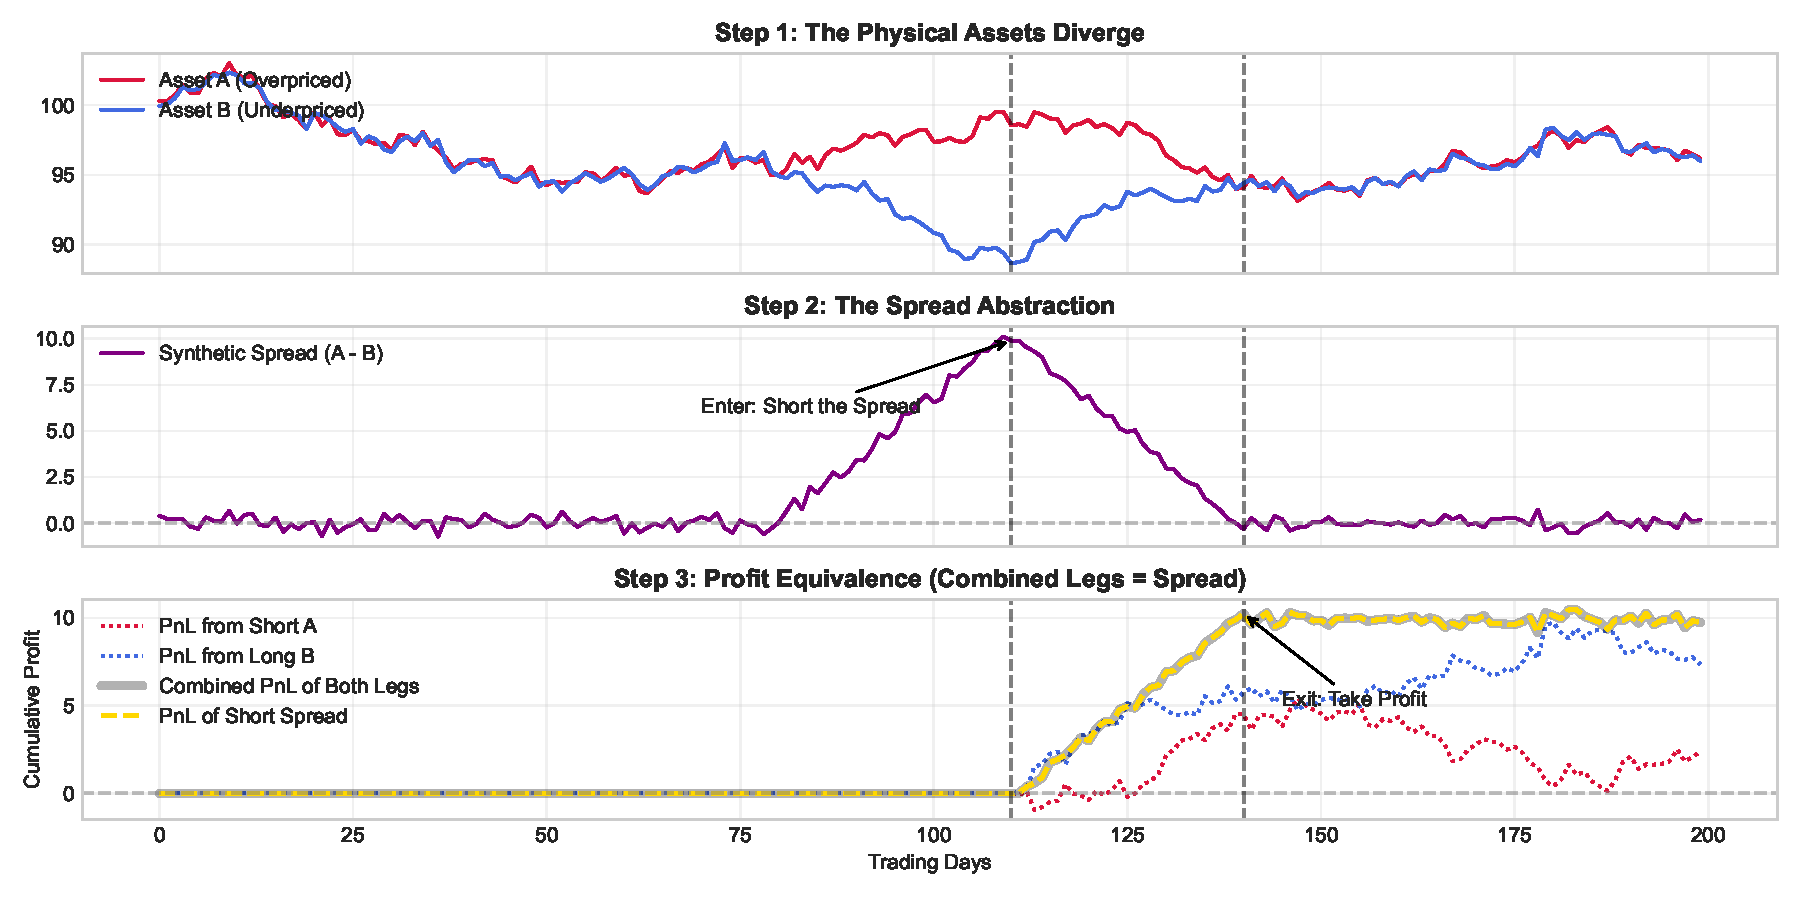
\includegraphics[width=\linewidth]{plots/long-short.pdf}
    \caption{Mechanics of a single pairs-trade. Top: the price path of each leg over the trade window. Bottom: the combined long/short portfolio, which is constructed to be exposed only to the relative move between the two legs and is approximately neutral to the common FX direction. The position is entered when the spread is far from its rolling mean (in $z$-score units) and closed as the spread reverts.}
    \label{fig:longshort}
\end{figure}

A do-nothing reference $\pi_t^{\mathrm{BH}} = +1$ for every $t$ (Buy \& Hold) earns $\Delta S_t$ at each step, pays no transaction costs, and provides a passive drift benchmark.

\subsection{Why the baseline is not enough}\label{sec:baselinelimits}

The baseline assumes $S_t$ is governed by a single stationary process, so that fixed $(z_q, z_x)$ correctly characterise ``far from equilibrium'' for every $t$. Two empirical features of FX tick data violate this assumption: (i) squared spread returns exhibit strong positive autocorrelation, consistent with conditional heteroskedasticity \parencite{engle1982arch,bollerslev1986garch,cont2001empirical}; and (ii) a spread that mean-reverts quickly in quiet periods may drift directionally for hundreds of bars during news-driven or one-sided-flow episodes \parencite{hasbrouck2007microstructure}. The fixed-threshold rule has no mechanism to distinguish these cases. This motivates the regime-aware extensions below.
%====================================================================
%   SECTION 4 — REGIME-AWARE MODELS
%====================================================================

\section{Regime-aware models}\label{sec:regimemodels}

We introduce the AR/HMM machinery on a generic series and then specialise to the spread $S_t$. The autoregressive model of order $p$ projects a series $Y_t$ on its $p$ most recent past values \parencite{hamilton1994},
\begin{equation}\label{eq:arp}
    Y_t \;=\; c \;+\; \phi_{1} Y_{t-1} \;+\; \cdots \;+\; \phi_{p} Y_{t-p} \;+\; \varepsilon_t, \qquad \varepsilon_t \overset{\mathrm{iid}}{\sim} \mathcal{N}(0,\sigma^{2}),
\end{equation}
with the simplest non-trivial case AR(1),
\begin{equation}\label{eq:ar1}
    Y_t \;=\; c + \phi\, Y_{t-1} + \varepsilon_t,
\end{equation}
having unconditional mean $c/(1-\phi)$ for $|\phi|<1$. AR(1) captures momentum ($\phi > 0$) or immediate mean reversion ($\phi < 0$) only if $(c,\phi,\sigma^{2})$ are constant over the sample; to relax that we let the parameters of \eqref{eq:ar1} be piecewise constant, switching with an unobserved discrete-time Markov chain $K_t \in \{1,\ldots,K\}$ \parencite{hamilton1989new}. The dynamics of $K_t$ are governed by a $K \times K$ transition matrix $\mathbf{P} = (p_{ij})$ and an initial distribution $\nu = (\nu_1,\ldots,\nu_K)^{\top}$,
\begin{equation}\label{eq:transitionmatrix}
    p_{ij} \;=\; \mathbb{P}(K_t = j \mid K_{t-1} = i),
    \qquad
    \nu_k \;=\; \mathbb{P}(K_1 = k),
\end{equation}
with the row-stochastic constraint $\sum_{j=1}^{K} p_{ij} = 1$ for every $i$. The Markov assumption is deliberately simple: the future depends on the past only through the current state, yet the framework is rich enough to capture persistence, sudden switching, and regime-dependent parameters within a single probabilistic model.

\subsection{Markov-switching AR(1) on the spread}\label{sec:msarspread}

We specialise to $S_t$ from \eqref{eq:rollingspreadret} and take $K = 2$. The joint generative model is
\begin{equation}\label{eq:msargen}
\begin{aligned}
    S_t \mid S_{t-1},\, K_t = k \;&\sim\; \mathcal{N}\!\bigl(c^{(k)} + \rho^{(k)} S_{t-1},\;(\sigma^{(k)})^{2}\bigr),\\[4pt]
    \mathbf{P} \;&=\; \begin{pmatrix} p_{11} & p_{12} \\ p_{21} & p_{22} \end{pmatrix},
\end{aligned}
\end{equation}
an AR(1) on the spread with all three parameters $(c^{(k)},\rho^{(k)},\sigma^{(k)})$ switching \parencite{krolzig1997msvar}. For $|\rho^{(k)}|<1$ the regime mean is $\mu^{(k)} = c^{(k)}/(1-\rho^{(k)})$, yielding the mean-deviation form
\begin{equation}\label{eq:meandevparam}
    S_t \;=\; \mu^{(k)} \;+\; \rho^{(k)}\bigl(S_{t-1} - \mu^{(k)}\bigr) \;+\; \varepsilon_t^{(k)},
    \qquad
    \varepsilon_t^{(k)} \;\sim\; \mathcal{N}\bigl(0,\,(\sigma^{(k)})^{2}\bigr).
\end{equation}
Values of $\rho^{(k)}$ close to zero correspond to fast mean reversion; values close to unity, to near-random-walk behaviour. Before estimation, $S_t$ is winsorised at $\mathrm{median}(S) \pm 4\cdot\mathrm{std}(S)$ and rescaled by $10^{4}$ for numerical stability.

\paragraph{Estimation, regime choice, and labelling.} The HMM parameter set
\begin{equation}\label{eq:thetadef}
    \Theta \;=\; \bigl\{\, \nu,\; \mathbf{P},\; c^{(k)},\; \rho^{(k)},\; \sigma^{(k)} : k=1,\ldots,K \,\bigr\}
\end{equation}
is estimated by maximum likelihood, fitted with the Markov-switching routine in the \texttt{statsmodels} package \parencite{seabold2010statsmodels} from multiple random starts to mitigate convergence to local maxima. The smoothed regime posteriors
\begin{equation}\label{eq:smoothedposterior}
    \gamma_t(k) \;=\; \mathbb{P}(K_t = k \mid S_1,\ldots,S_T;\Theta)
\end{equation}
fall out of the same fit. We fix $K = 2$ throughout, motivated by the regime-switching literature in which a parsimonious two-state model already captures the dominant non-stationarity in returns \parencite{hamilton1989new}; in preliminary exploration $K \in \{3, 4\}$ either failed to separate cleanly across seeds or split the high-volatility state into sub-regimes whose entry implications were indistinguishable at the relevant cost level. With $K=2$ we label regimes by innovation variance,
\begin{equation}\label{eq:regimelabels}
    k_{\mathrm{MR}} \;=\; \arg\min_{k}\,\sigma^{(k)},
    \qquad
    k_{\mathrm{DR}} \;=\; \arg\max_{k}\,\sigma^{(k)},
\end{equation}
giving a mean-reverting (MR) and a drifting (DR) regime, with $\gamma_t^{\mathrm{MR}} = \mathbb{P}(K_t = k_{\mathrm{MR}} \mid S_1,\ldots,S_T)$ and $\gamma_t^{\mathrm{DR}} = 1 - \gamma_t^{\mathrm{MR}}$. In live trading only past observations are available, so the filtered posterior $\mathbb{P}(K_t = k_{\mathrm{MR}} \mid S_1,\ldots,S_t)$ is used inside the walk-forward back-test while the smoothed posterior is reserved for diagnostic figures.

\subsection{Regime-aware strategies}\label{sec:regimestrategies}

We build two regime-aware strategies on top of the baseline \eqref{eq:baselinerule}. Both inherit the baseline's entry direction and exit logic without modification: at every bar the candidate position is $\pi_t^{\mathrm{baseline}}$ from \eqref{eq:baselinerule}, and the regime model can only veto or attenuate that candidate. Neither variant can generate a position the baseline did not generate, nor reverse a position the baseline took.

\paragraph{AR-gated.} A binary gate with danger threshold $\delta \in (0,1)$,
\begin{equation}\label{eq:argate}
    G_t \;=\; \mathbbm{1}\!\bigl\{\,\gamma_t^{\mathrm{MR}} \,\geq\, 1-\delta\,\bigr\},
\end{equation}
modifies the rule to
\begin{equation}\label{eq:arpositionrule}
    \pi_t \;=\;
    \begin{cases}
        0 & \text{if } G_t = 0 \quad\text{(liquidate, stay flat)},\\[2pt]
        \pi_t^{\mathrm{baseline}} & \text{if } G_t = 1.
    \end{cases}
\end{equation}
The gate is binary: trade exactly like the baseline, or sit in cash. It also applies to existing positions: if we are long the spread and the HMM flags danger, the position goes flat at the next bar.

\paragraph{MS-AR.} A continuous, regime-weighted entry threshold,
\begin{equation}\label{eq:msarthreshold}
    z_q^{\mathrm{eff}}(t) \;=\; \gamma_t^{\mathrm{MR}}\, z_q \;+\; \gamma_t^{\mathrm{DR}}\, z_v,
    \qquad\text{with } z_v \geq z_q,
\end{equation}
replaces $z_q$ in \eqref{eq:baselinerule} by $z_q^{\mathrm{eff}}(t)$. When MR is highly probable, $z_q^{\mathrm{eff}} \approx z_q$ and the strategy trades like the baseline; when DR dominates, a larger $|Z_t|$ deviation is required before entering.

Table~\ref{tab:strategy_definitions} summarises the four strategies compared throughout the rest of the thesis. All three active rules share the cointegration spread $S_t$ and its $z$-score $Z_t$ and differ only in whether and how $\gamma_t^{\mathrm{MR}}$ enters the decision. In particular, AR and MS-AR are not separate forecasters; on any bar where the HMM does not intervene they trade exactly like the baseline, so any difference in performance between baseline and the regime-aware variants is attributable entirely to the gate suppressing or attenuating baseline trades.

\begin{table}[H]
\centering
\caption{The four strategies compared in this thesis. The ``Gate'' column gives the indicator multiplying the baseline position $\pi_t^{\mathrm{baseline}}$ before it is taken; a value of $1$ means the baseline is always allowed to trade.}
\label{tab:strategy_definitions}
\small
\begin{tabular}{lllll}
\toprule
\textbf{Strategy} & \textbf{Always long?} & \textbf{Entry threshold} & \textbf{Gate} & \textbf{Reads HMM?} \\
\midrule
Buy \& Hold & Yes & n/a & n/a & No \\
Baseline    & No  & $z_q$ & $1$ & No \\
AR          & No  & $z_q$ & $\mathbbm{1}\{\gamma_t^{\mathrm{MR}} \geq 1-\delta\}$ & Yes (binary) \\
MS-AR       & No  & $\gamma_t^{\mathrm{MR}} z_q + \gamma_t^{\mathrm{DR}} z_v$ & $1$ & Yes (continuous) \\
\bottomrule
\end{tabular}
\end{table}

%====================================================================
%   SECTION 5 — BACK-TEST PROTOCOL AND METRICS
%====================================================================

\section{Back-test protocol and metrics}\label{sec:backtest}

\paragraph{Costs and walk-forward.}\label{sec:walkforward}
Every position change in leg $i$ pays the half-spread $\mathrm{HS}_t^{\,i}$ of \eqref{eq:midprice} plus a fixed commission \parencite{aldridge2013hft}, so the round-trip cost of one pair-position is approximately $\mathrm{HS}^{A} + \hat\beta\,\mathrm{HS}^{B}$ in basis points. Strategies are evaluated walk-forward: parameters $\Theta$ and hyperparameters $(W_\beta, W_z, z_q, z_x, z_v, \delta)$ are fitted on a training segment and applied to a disjoint out-of-sample test segment, with windows slid forward \parencite{lopezdeprado2018advances}.

\paragraph{Core performance metrics.}\label{sec:metrics}
We report three core metrics in the body of the thesis: annualised volatility, the Sharpe ratio, and the maximum drawdown. A fuller set of distributional, tail-risk, and risk-adjusted diagnostics (skewness, excess kurtosis, VaR, CVaR, Sortino, Calmar, Ulcer index) is collected in Appendix~\ref{sec:apx-extra-metrics} and reported in the per-pair tearsheets. Let $R_t$ denote the strategy return at bar $t$, $\mu_R = \mathbb{E}[R]$, $\sigma_R = \sqrt{\mathrm{Var}(R)}$, $V_t$ the portfolio value with running peak $V_t^{\star} = \max_{s \leq t} V_s$, and $R_f$ a benchmark risk-free rate (set to zero). The three core metrics are
\begin{equation}\label{eq:coremetrics}
    \sigma_{\mathrm{ann}} \;=\; \sigma_R\sqrt{T},
    \qquad
    \mathrm{SR} \;=\; \frac{\mu_R - R_f}{\sigma_R},
    \qquad
    \mathrm{MDD} \;=\; \max_{t}\,\frac{V_t^{\star} - V_t}{V_t^{\star}},
\end{equation}
covering scale (volatility), risk-adjusted return (Sharpe \parencite{sharpe1994ratio}), and worst-case capital loss (maximum drawdown). Trade-level diagnostics (win rate, market exposure, profit factor, payoff ratio) summarise frequency and size; see Section~\ref{sec:result} for their interpretation.

\section{Result}
\label{sec:result}

Figure~\ref{fig:eurusd-tick-analysis} presents an exploratory data analysis of EUR/USD tick data for January 2026. The top panel shows that the mid-price evolves broadly continuously but with intermittent jumps, while the bid-ask spread is highly concentrated at the minimum tick size with an extended right tail characteristic of illiquid periods. The middle panel reveals strong intraday seasonality in the spread, with compression during the overlapping London--New York session and widening during the Asian session and around macroeconomic announcements; the distribution of one-minute log returns exhibits the heavy tails and excess kurtosis typical of high-frequency data. The bottom panel confirms that trading intensity peaks at market open and at the US open, and that annualised daily realised volatility fluctuates substantially across the month---evidence of the time-varying dependence structure that the HMM framework is designed to capture.

\begin{figure}[h!]
    \centering
    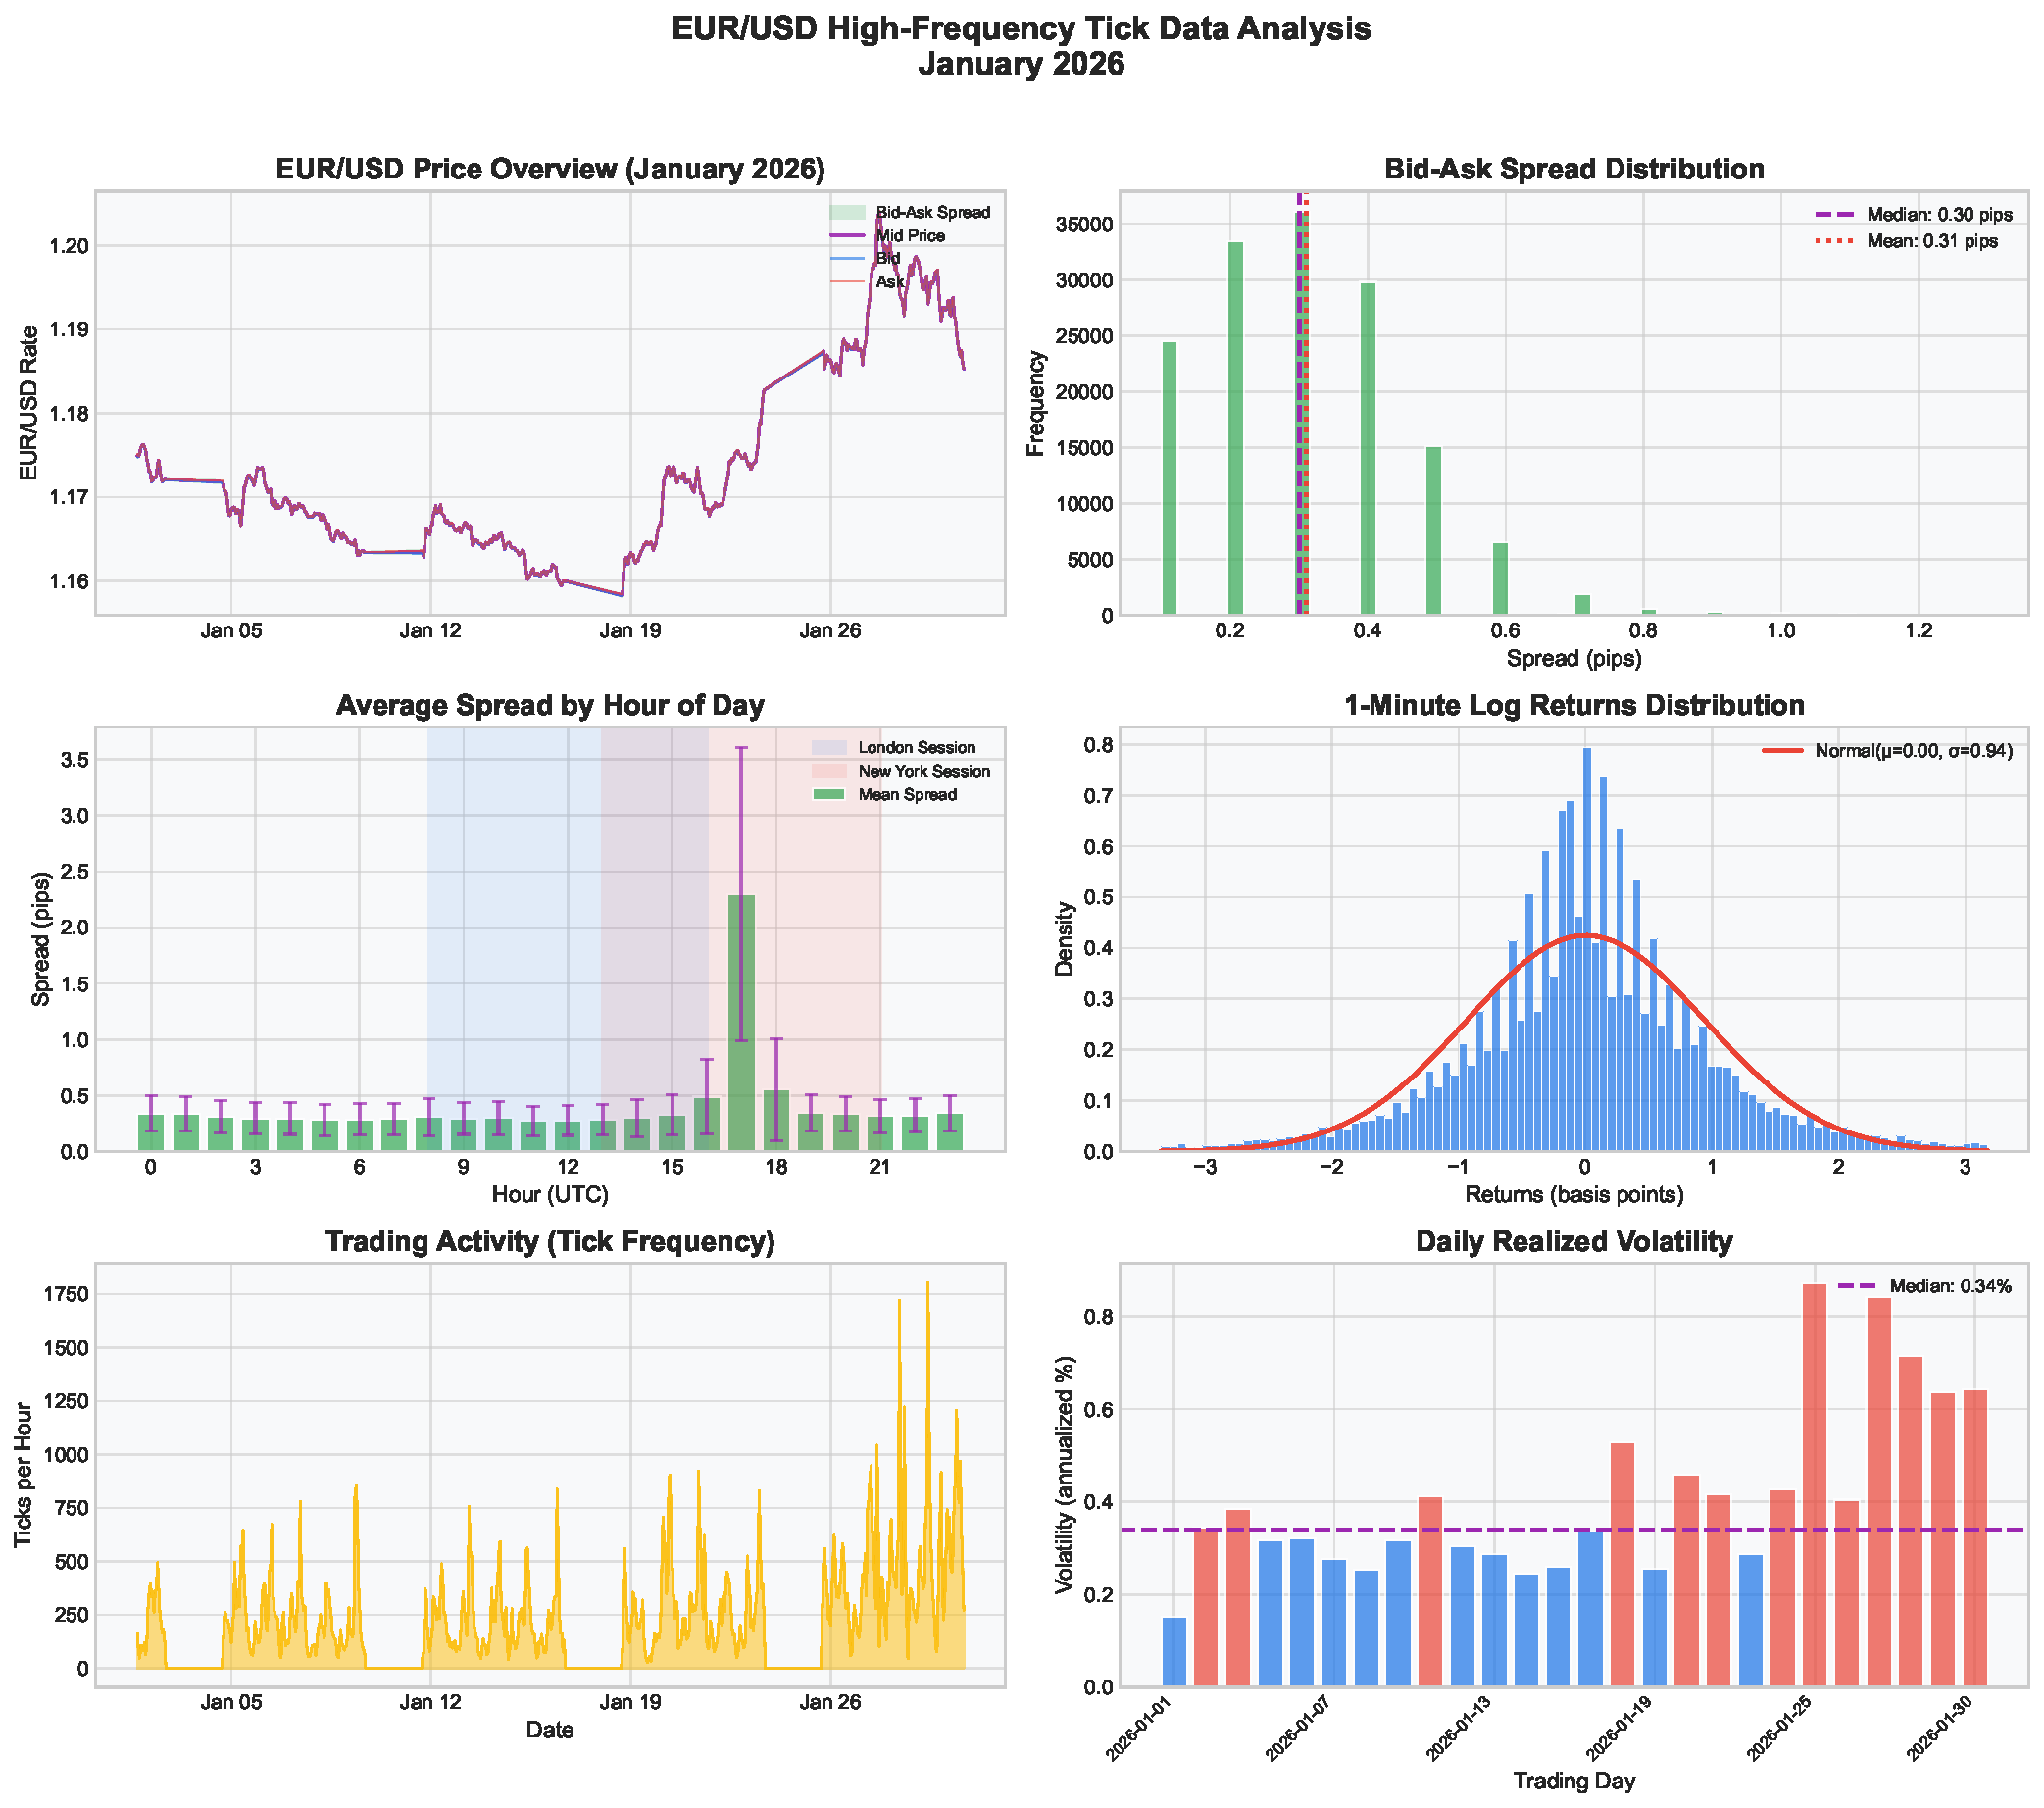
\includegraphics[width=0.6\linewidth]{plots/eurusd_tick_analysis.pdf}
    \caption{Exploratory data analysis of EUR/USD tick data for January 2026. The panels display the price evolution and bid-ask spread distribution (top); intraday spread seasonality highlighting the London and New York sessions, alongside the leptokurtic distribution of 1-minute log returns compared to a Gaussian benchmark (middle); and hourly trading activity frequency alongside annualized daily realized volatility (bottom).}
    \label{fig:eurusd-tick-analysis}
\end{figure}
\section{Conclusion}\label{sec:conclusion}

This thesis has tested whether Hidden Markov Models add value to a classical pairs-trading rule on high-frequency FX tick data. The exercise was deliberately layered: a single baseline signal---the rolling $z$-score of the cointegration spread \parencite{engle1987cointegration,gatev2006pairs,vidyamurthy2004pairs}---was first treated as a self-contained strategy and back-tested under realistic transaction costs and a per-day fit \parencite{aldridge2013hft,lopezdeprado2018advances,seabold2010statsmodels,lam2015numba}; the HMM was then introduced as a regime gate \parencite{hamilton1989new,rabiner1989tutorial,krolzig1997msvar}, with two concrete instantiations---a binary AR-gated rule and a probability-weighted MS-AR threshold---that leave the baseline's directional entry rule unchanged.

\subsection{Summary of findings}\label{sec:concl-findings}

\begin{enumerate}
    \item \textbf{The cointegration baseline is unprofitable at realistic frictions.} Across all three pair constructions and all three monthly episodes (August 2024, December 2024, April 2025), the rolling $z$-score rule generates a stream of round-trips at small per-trade alpha and bleeds net of the half-spread plus commission. Sharpe ratios are negative everywhere, ranging from $-17$ on the cheapest pair--month to $-126$ on the highest-spread one (Table~\ref{tab:result_headline}). The pair-level magnitude of damage is monotone in the per-leg half-spread, which is the cleanest causal statement we can make from the data \parencite{krauss2017statarb,roll1984spread}.
    \item \textbf{The HMM gate is a defensive filter, not a return enhancer.} Both regime-aware strategies sharply reduce market exposure (typically from $\sim 30\%$ for the Baseline to $5$--$15\%$ for AR and $6$--$17\%$ for MS-AR), the number of round-trips (by a factor of three to five), annualised volatility, and the Ulcer index of \textcite{martin1989ulcer}. Cumulative loss is roughly $75$--$85\%$ smaller on every pair--month, but never crosses into profit \parencite{sharpe1994ratio,sortino1991downside}.
    \item \textbf{MS-AR does not improve on the binary AR gate.} The continuous, regime-weighted threshold of \eqref{eq:msarthreshold} produces equity curves that are nearly indistinguishable from---and on cumulative PnL consistently slightly worse than---the binary danger gate of \eqref{eq:argate}. The extra parameter $z_v$ admits a few marginal entries that are net-negative at this cost level; a BIC-style penalty \parencite{schwarz1978bic} on the additional parameter would already select against MS-AR. This is an honest negative finding on the value of the extra parameter, consistent with the caution of \textcite{cappe2005} that smoothing a regime decision rule is only beneficial when the marginal entries it admits are profitable in expectation.
    \item \textbf{Buy~\&~Hold dominates the active strategies in seven of nine pair--months.} The passive long-spread reference is positive in six of nine cells and is the only positive Sharpe in any column on EUR/NOK--EUR/SEK in December 2024 and April 2025, and on GBP/USD--EUR/USD in all three months. The most striking single comparison is EUR/NOK--EUR/SEK in April 2025: passive drift earns $+528\,\text{bps}$ on the same spread that the cointegration rule loses $-19{,}906\,\text{bps}$ on. At these frictions, doing nothing beats the textbook rule on every pair we tested.
    \item \textbf{The model is interpretable.} The EM/Baum--Welch fits \parencite{baum1970maximization,dempster1977} of the Markov-switching AR(1) recover two regimes with well-separated innovation variances, posterior persistences close to one for the mean-reverting state, and means $\mu^{(k)}$ close to zero (Figure~\ref{fig:regime-dynamics}). The smoothed posterior tracks quiet versus turbulent stretches within each session; the negative result on profitability therefore cannot be blamed on a misbehaving model \parencite{cappe2005}.
\end{enumerate}

The central contribution is not a claim that HMMs universally outperform simpler models---they do not---but a careful, costed, per-day-fit test of when regime awareness helps, when it fails, and how mathematical models behave when confronted with noisy, costly, non-stationary tick data \parencite{cont2001empirical,hautsch2012econometrics}.

\subsection{Limitations and future directions}\label{sec:concl-future}

The exercise is restricted to three pair constructions, three independent one-month sub-samples, $K=2$ regimes fitted day by day, unit-size long/flat/short positions, a half-spread-plus-commission cost model that omits latency and market impact \parencite{aldridge2013hft}, and an in-sample smoothed posterior for the AR/MS-AR gates---a strictly out-of-sample forward filter is deferred to follow-up work. The negative finding is therefore best read as a statement about the textbook cointegration $z$-score rule under realistic FX frictions, not about HMMs as such. A second caveat: the three months were chosen for active price movement under structurally different macro backdrops, which is good for cross-episode robustness but biases the sample toward periods in which a passive long-spread position can drift directionally; the Buy~\&~Hold advantage in two of the three months should be read as a property of the chosen episodes rather than as a universal claim.

Three extensions follow naturally. The most direct is to \emph{combine the regime posteriors with a different entry signal in the drifting regime}---for example a momentum signal of the kind used in \textcite{avellaneda2010statarb}---rather than asking the HMM to gate a mean-reversion signal that is already cost-dominated. The negative result tells future work where \emph{not} to spend complexity budget. A second is to \emph{pre-screen the pair universe with the baseline back-test before applying the HMM}: the cost-ordering of our three pairs is so clean that a single Baseline back-test eliminates the high-spread pair, regardless of any regime gate \parencite{krauss2017statarb}. A third is to \emph{replace the per-day in-sample smoothing with a true walk-forward filter}, using only past observations to form $\mathbb{P}(K_t = k_{\text{MR}} \mid S_1,\ldots,S_t)$; this is the conservative direction in which to push the result---the filter is a strict subset of the smoother's information set, so a walk-forward implementation can only lower the value of the regime gate further, and it therefore tightens rather than weakens the negative conclusion. A further direction is an HMM--GARCH hybrid \parencite{bollerslev1986garch,engle1982arch} that lets the within-regime conditional variance evolve smoothly between switches, a natural fit for the heavy-tailed conditionally heteroskedastic distributions of Figure~\ref{fig:res-audnzd-rd-grid}. The full reproducible implementation---data pipeline, back-test driver, daily ledgers, and per-pair tearsheets---is released as the open-source repository \texttt{stk-mat2011} \parencite{furnes2026repo} as a starting point for those follow-ups.

\clearpage
\printbibliography
\newpage
\section{Appendix}\label{sec:appendix}

%%%
\subsection{Three-month cumulative-PnL panels (symlog)}\label{sec:apx-strategy-panels}

Symlog-scaled cumulative-PnL panels stacking the four strategies (Buy~\&~Hold, Baseline, AR, MS-AR) across the three monthly episodes for each pair.

\begin{figure}[H]
    \centering
    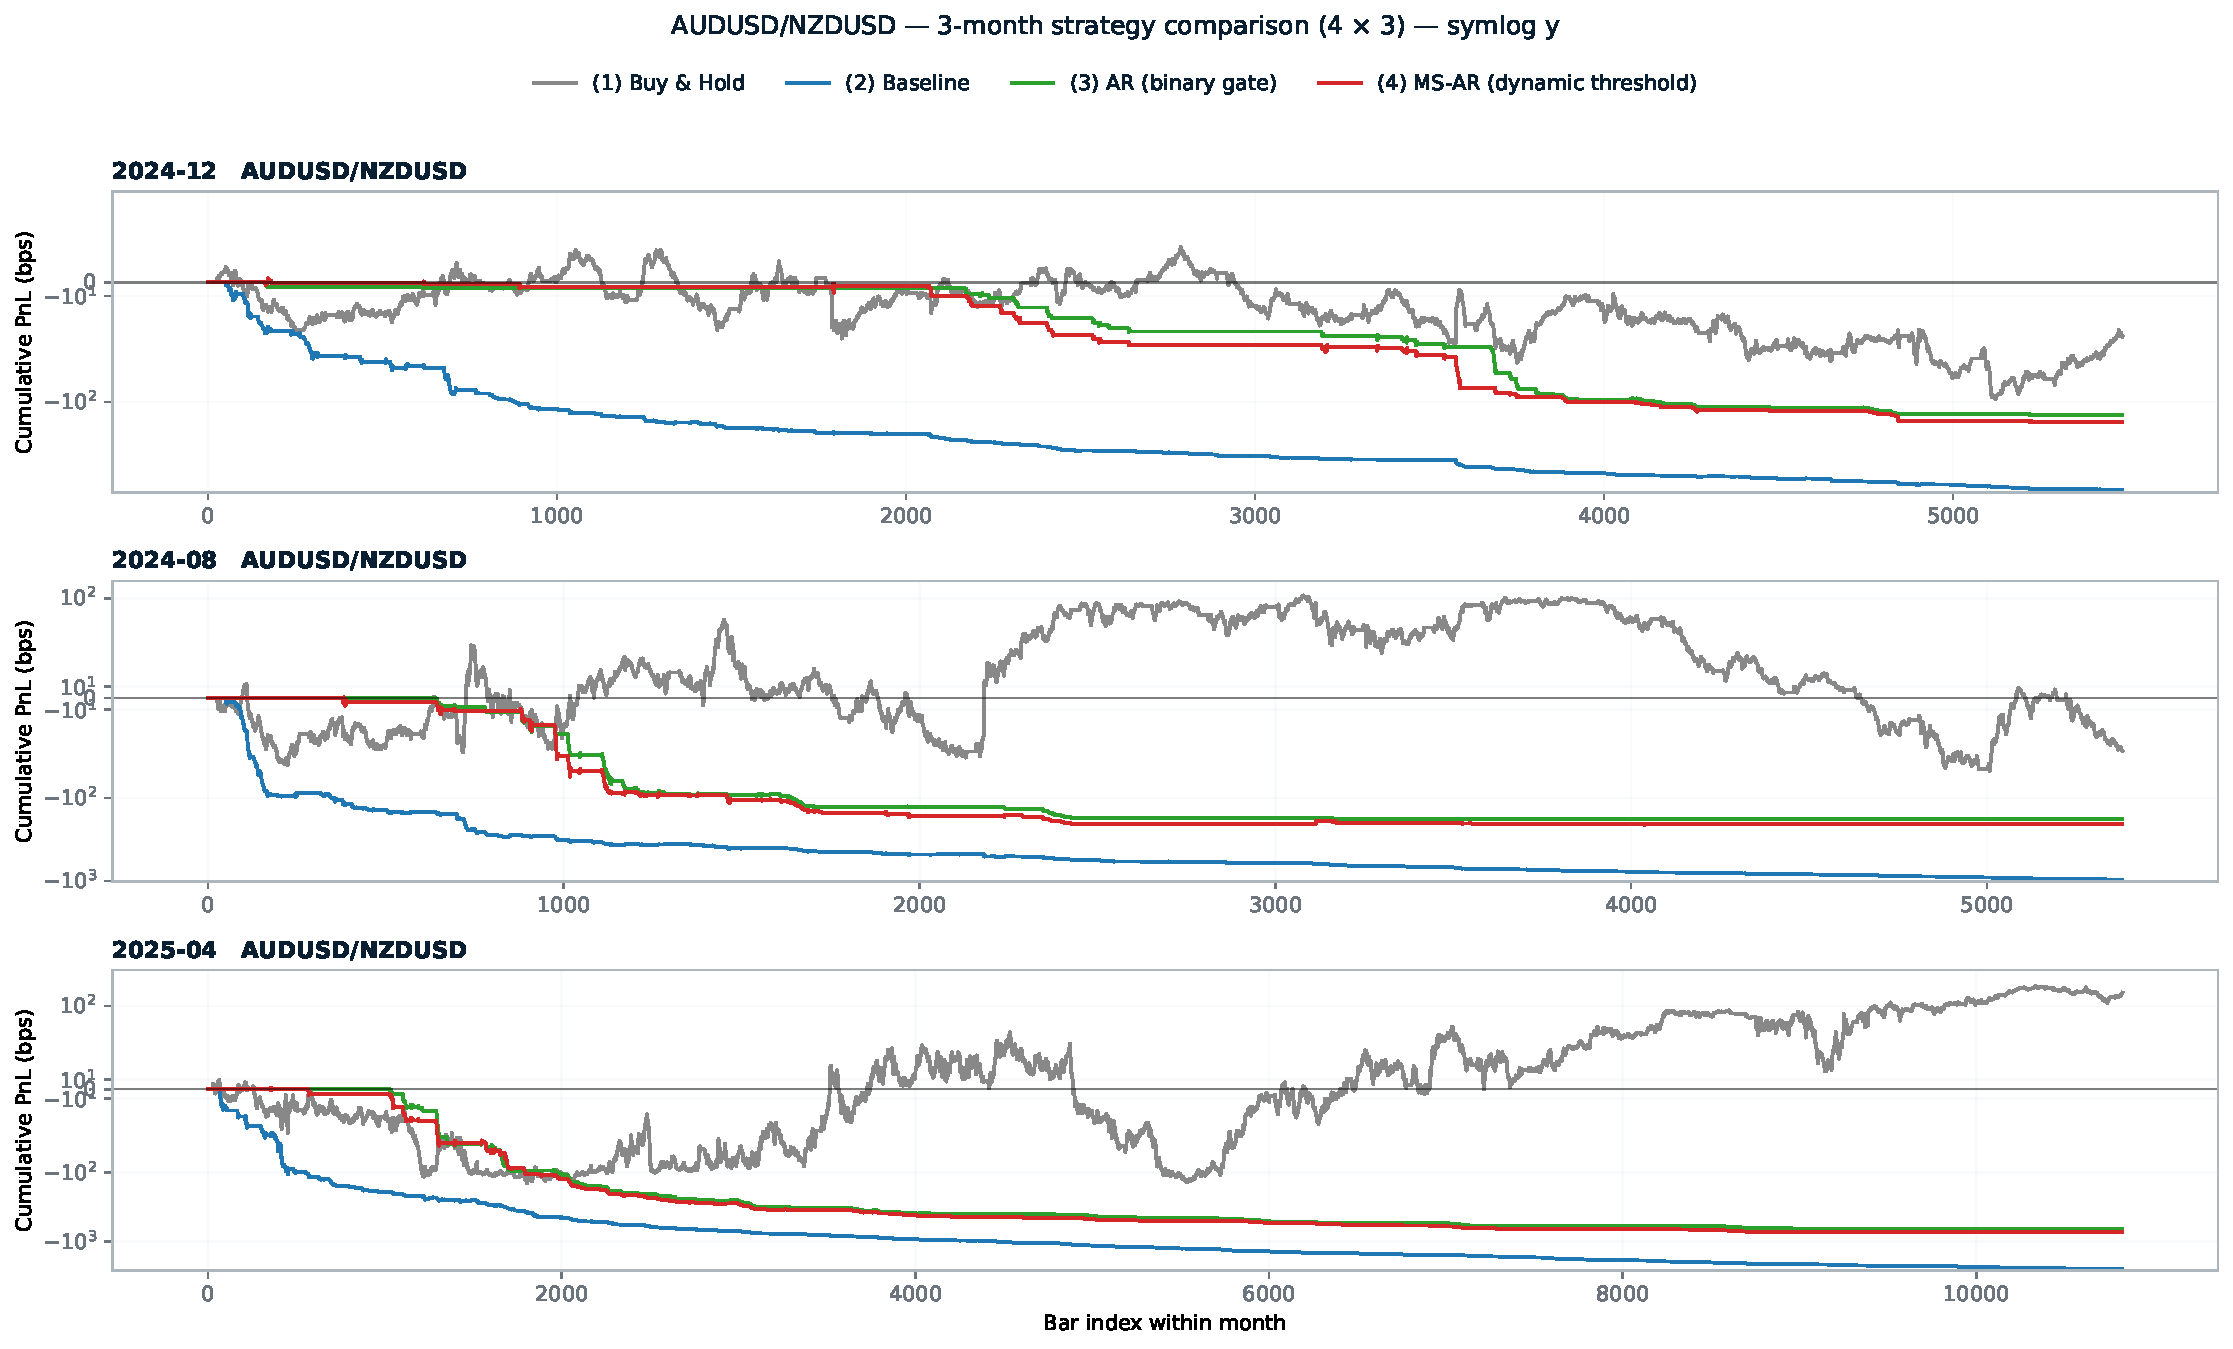
\includegraphics[width=\linewidth]{plots/AUDUSD_NZDUSD_three_month_strategy_panel_symlog.pdf}
    \caption{AUD/USD--NZD/USD, three-month strategy comparison on a symmetric-log $y$-axis.}
    \label{fig:apx-audnzd-three-month-symlog}
\end{figure}

\begin{figure}[H]
    \centering
    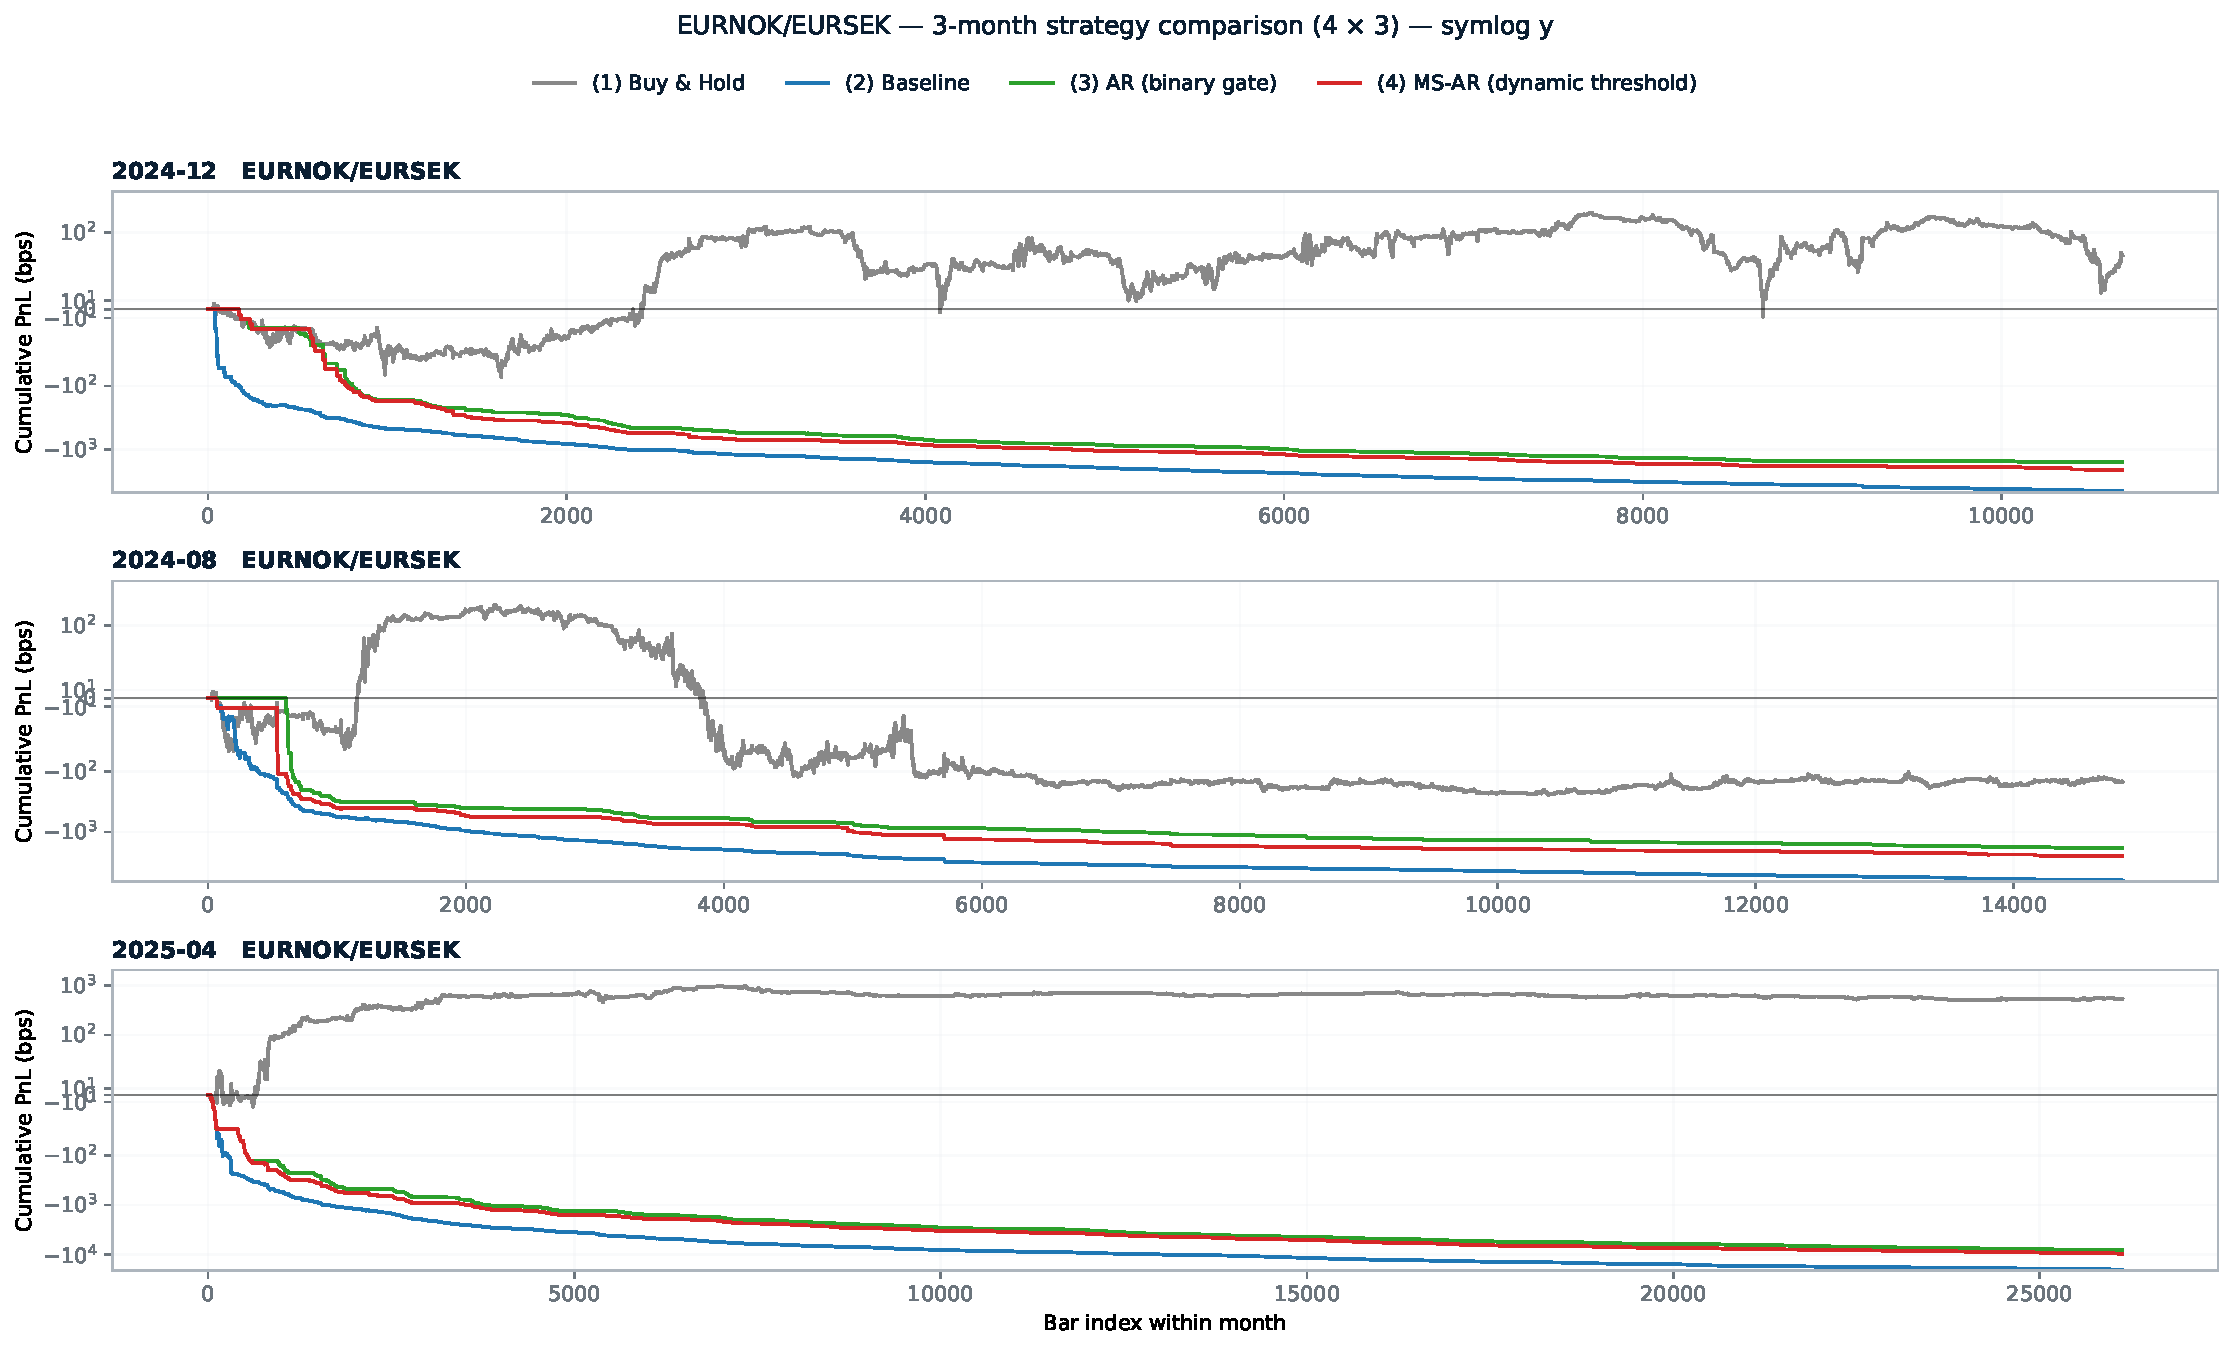
\includegraphics[width=\linewidth]{plots/EURNOK_EURSEK_three_month_strategy_panel_symlog.pdf}
    \caption{EUR/NOK--EUR/SEK, three-month strategy comparison on a symmetric-log $y$-axis.}
    \label{fig:apx-noksek-three-month-symlog}
\end{figure}

\begin{figure}[H]
    \centering
    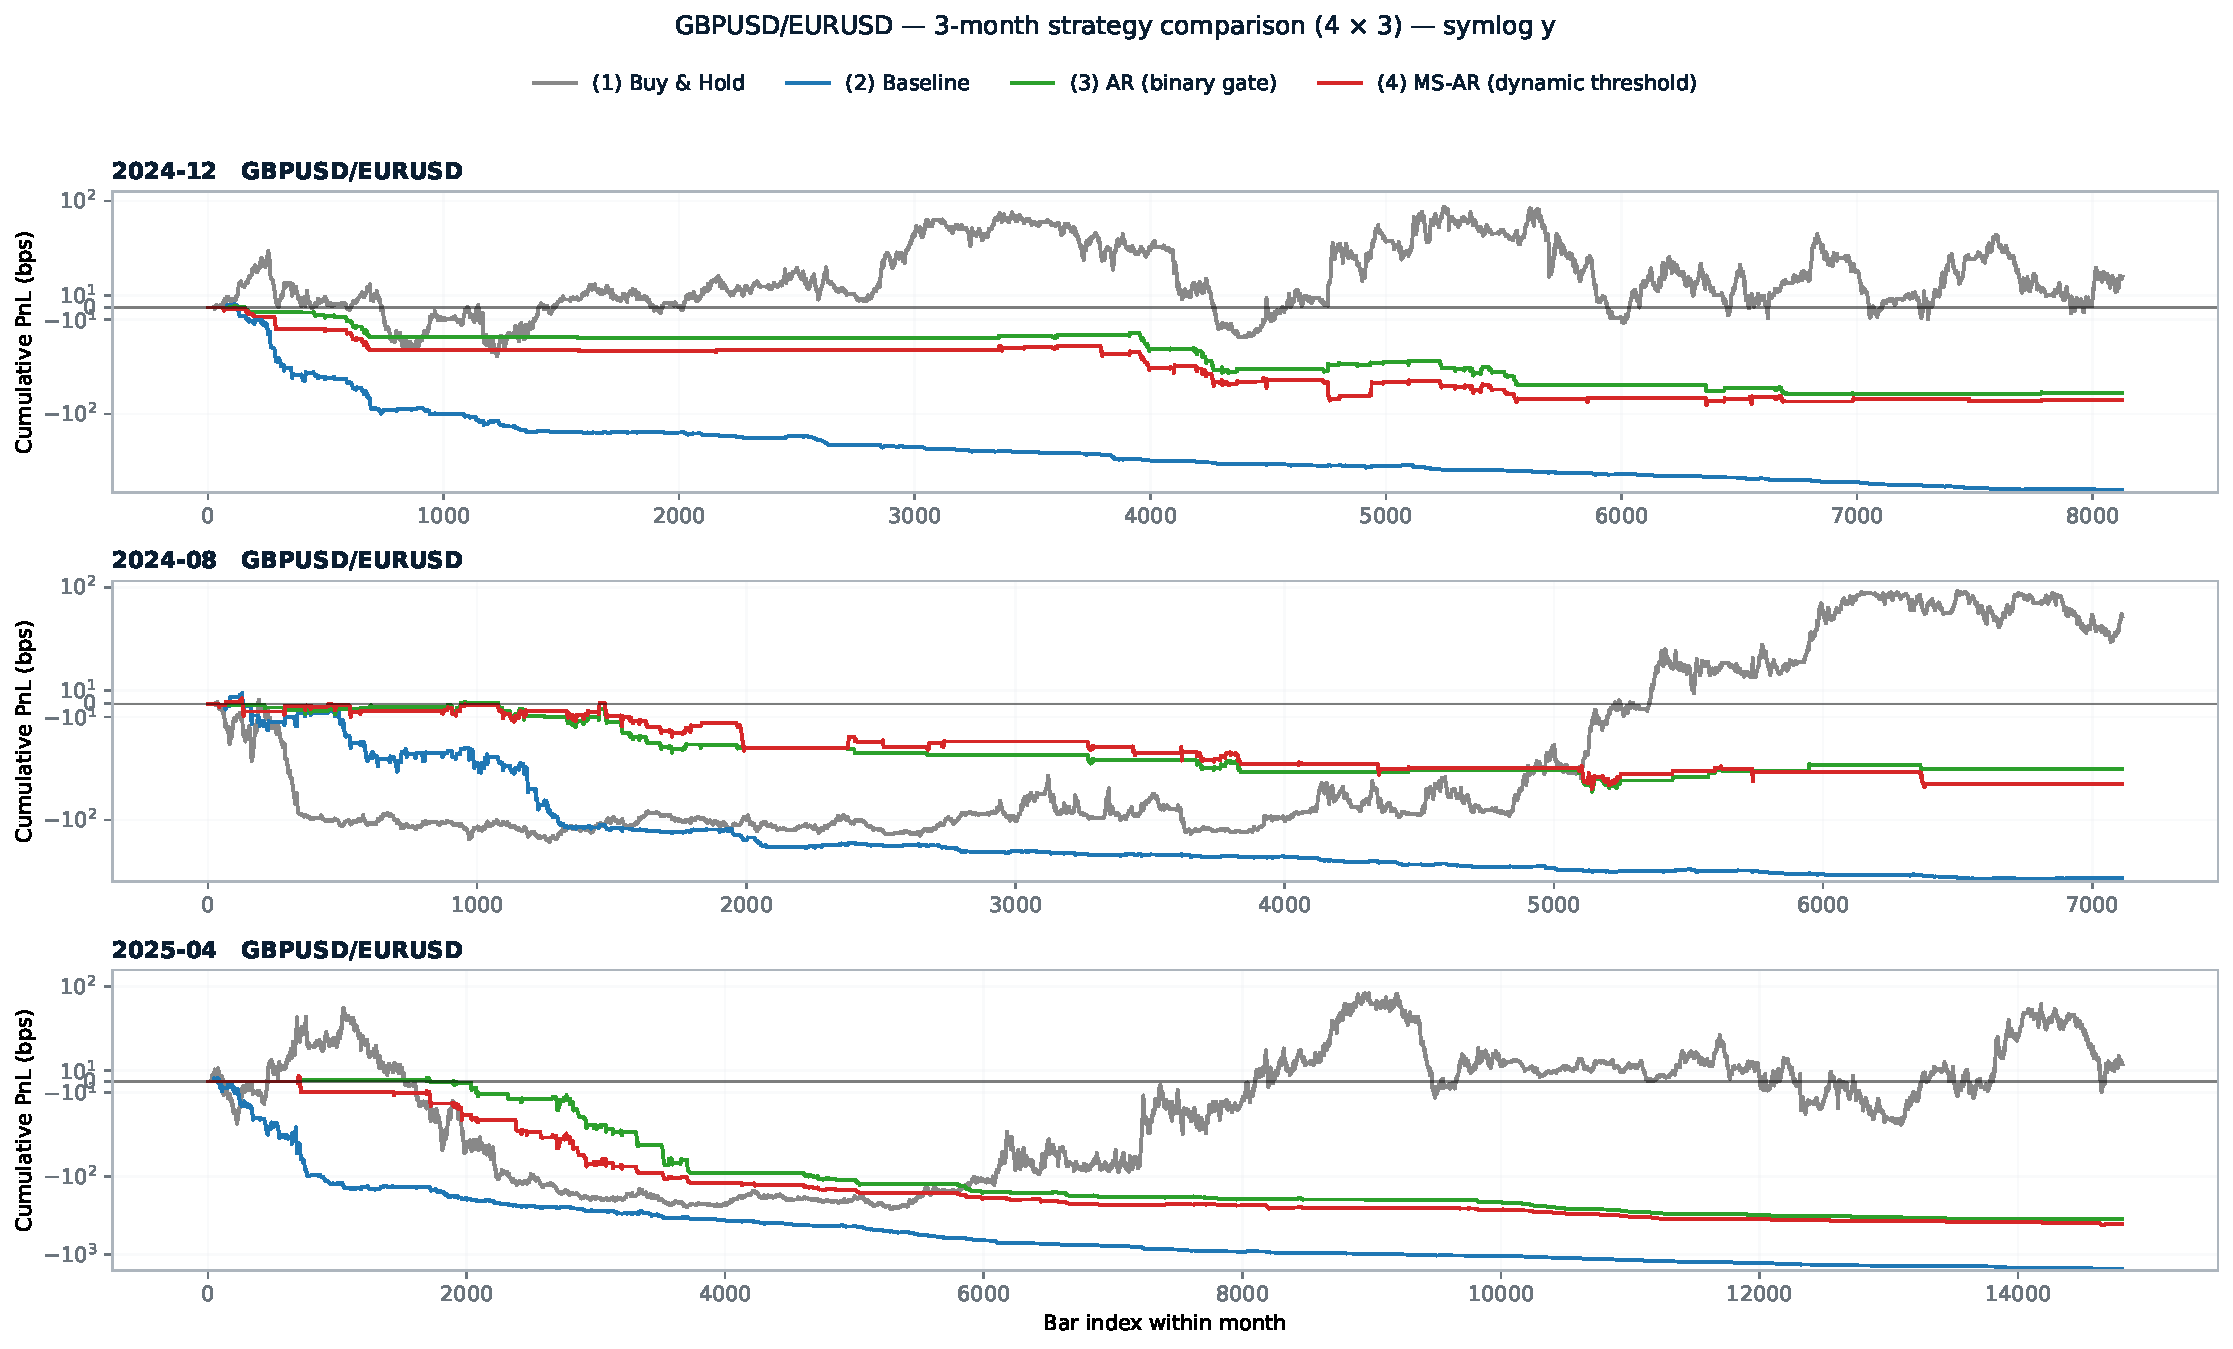
\includegraphics[width=\linewidth]{plots/GBPUSD_EURUSD_three_month_strategy_panel_symlog.pdf}
    \caption{GBP/USD--EUR/USD, three-month strategy comparison on a symmetric-log $y$-axis.}
    \label{fig:apx-gbpeur-three-month-symlog}
\end{figure}
\clearpage

\subsection{MS-AR equity overlays by month}\label{sec:apx-msar-overlays}

Per-pair MS-AR equity curves overlaid across the three monthly episodes (August 2024, December 2024, April 2025).

\begin{figure}[H]
    \centering
    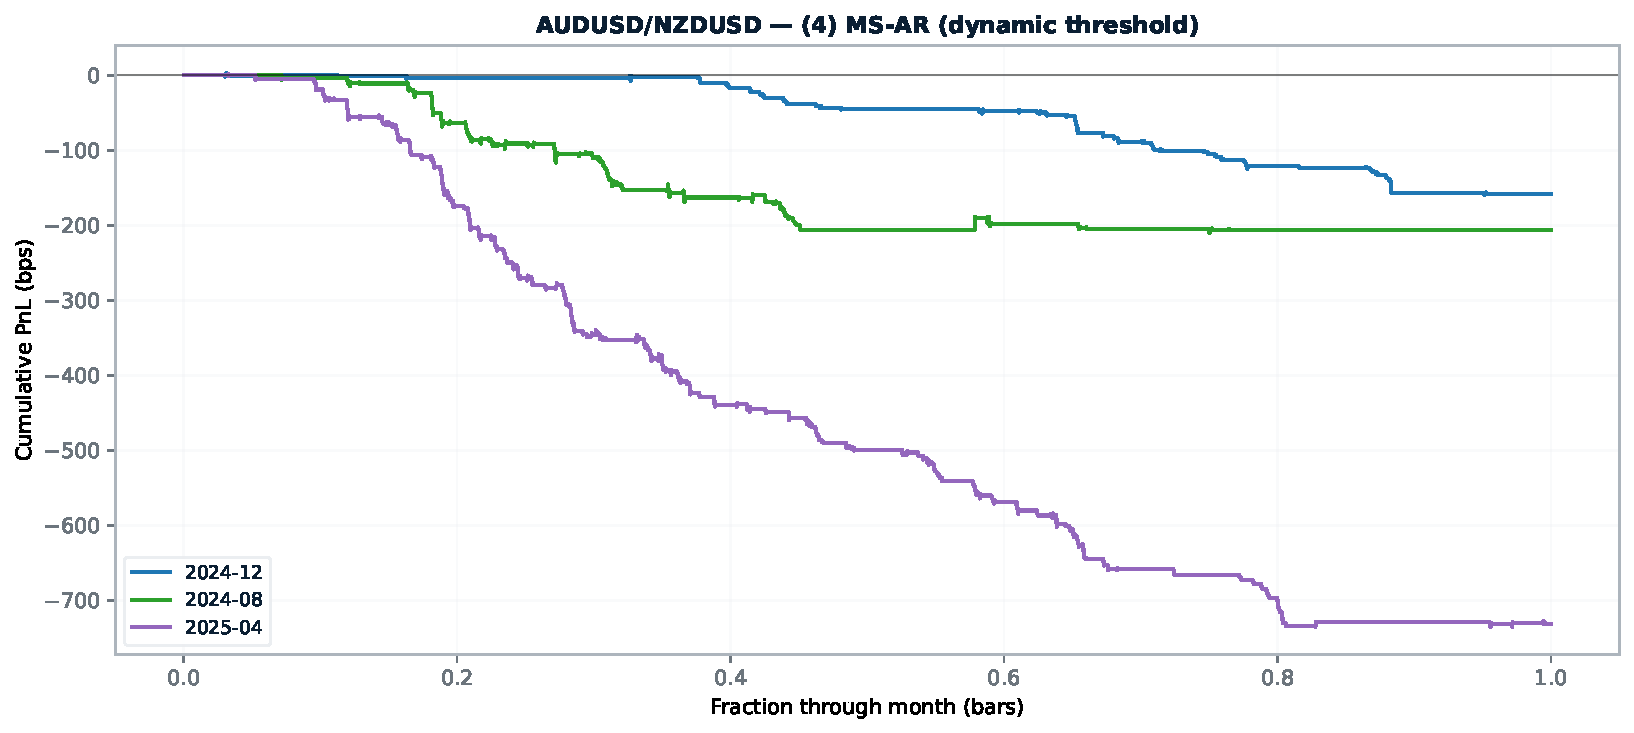
\includegraphics[width=0.7\linewidth, height=0.28\textheight, keepaspectratio]{plots/AUDUSD_NZDUSD_MS_AR_by_month_overlay.pdf}\\[0.4em]
    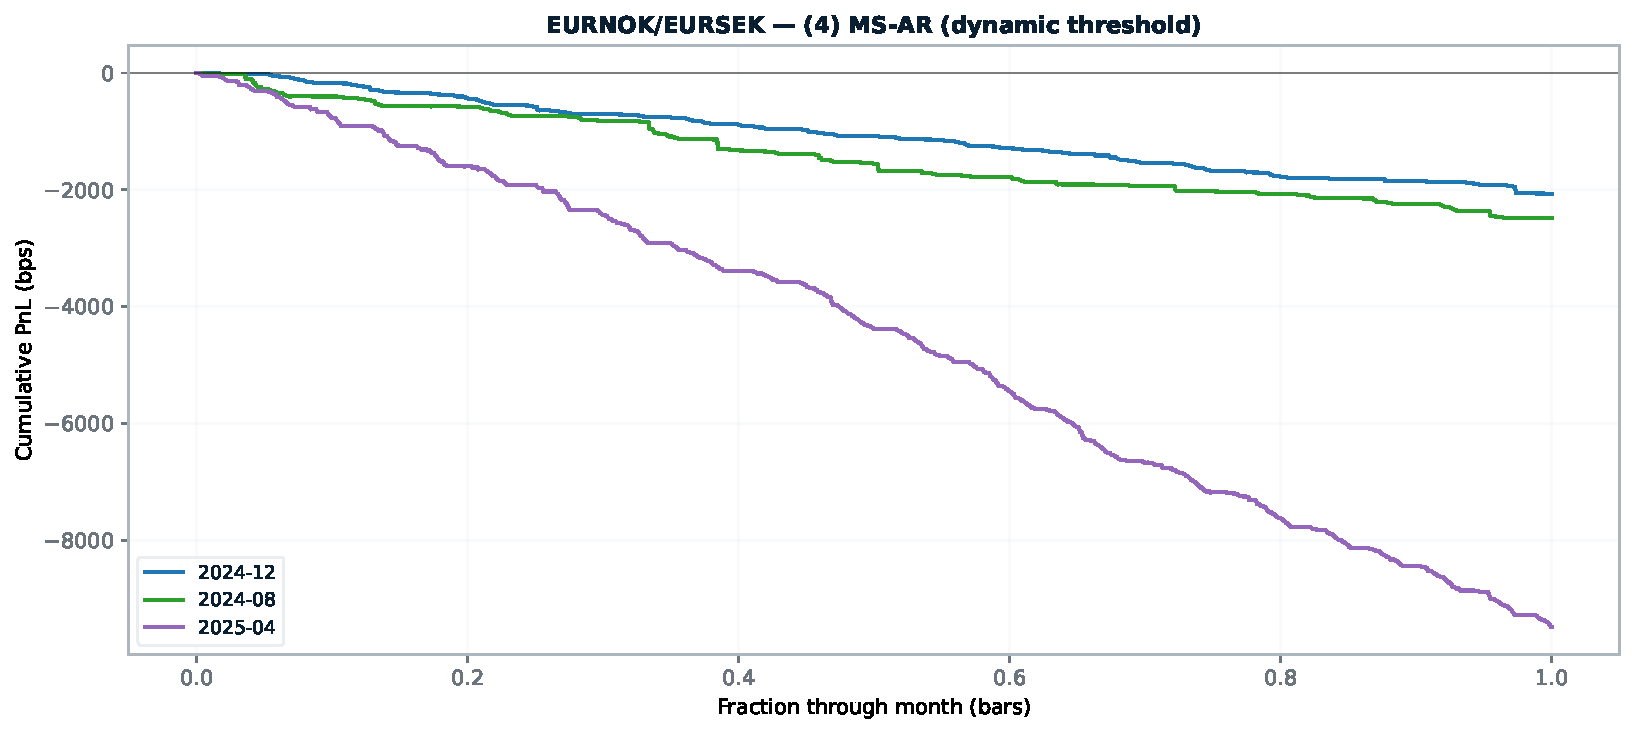
\includegraphics[width=0.7\linewidth, height=0.28\textheight, keepaspectratio]{plots/EURNOK_EURSEK_MS_AR_by_month_overlay.pdf}\\[0.4em]
    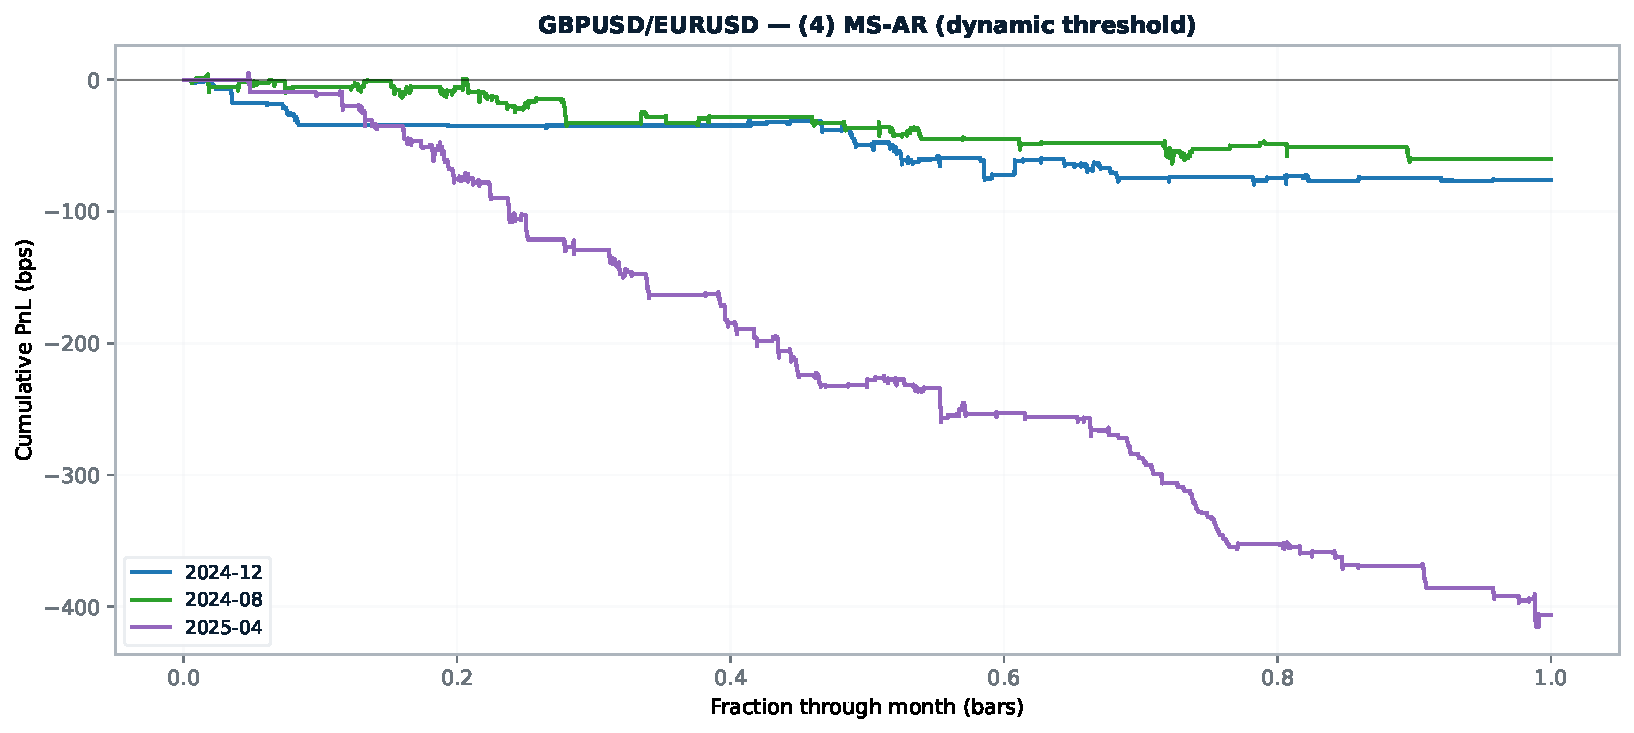
\includegraphics[width=0.7\linewidth, height=0.28\textheight, keepaspectratio]{plots/GBPUSD_EURUSD_MS_AR_by_month_overlay.pdf}
    \caption{MS-AR equity overlay by month. Top: AUD/USD--NZD/USD; middle: EUR/NOK--EUR/SEK; bottom: GBP/USD--EUR/USD.}
    \label{fig:apx-msar-overlay-grid}
\end{figure}
\clearpage

\subsection{Positions and regime gates}\label{sec:apx-positions-regimes}

Bar-by-bar Baseline positions overlaid with the HMM-implied regime gate, for the August 2024 episode of each pair. Shaded windows mark bars in which the AR gate $G_t = 0$ forces a liquidation. The remaining months are available in the companion repository \parencite{furnes2026repo}.

\begin{figure}[H]
    \centering
    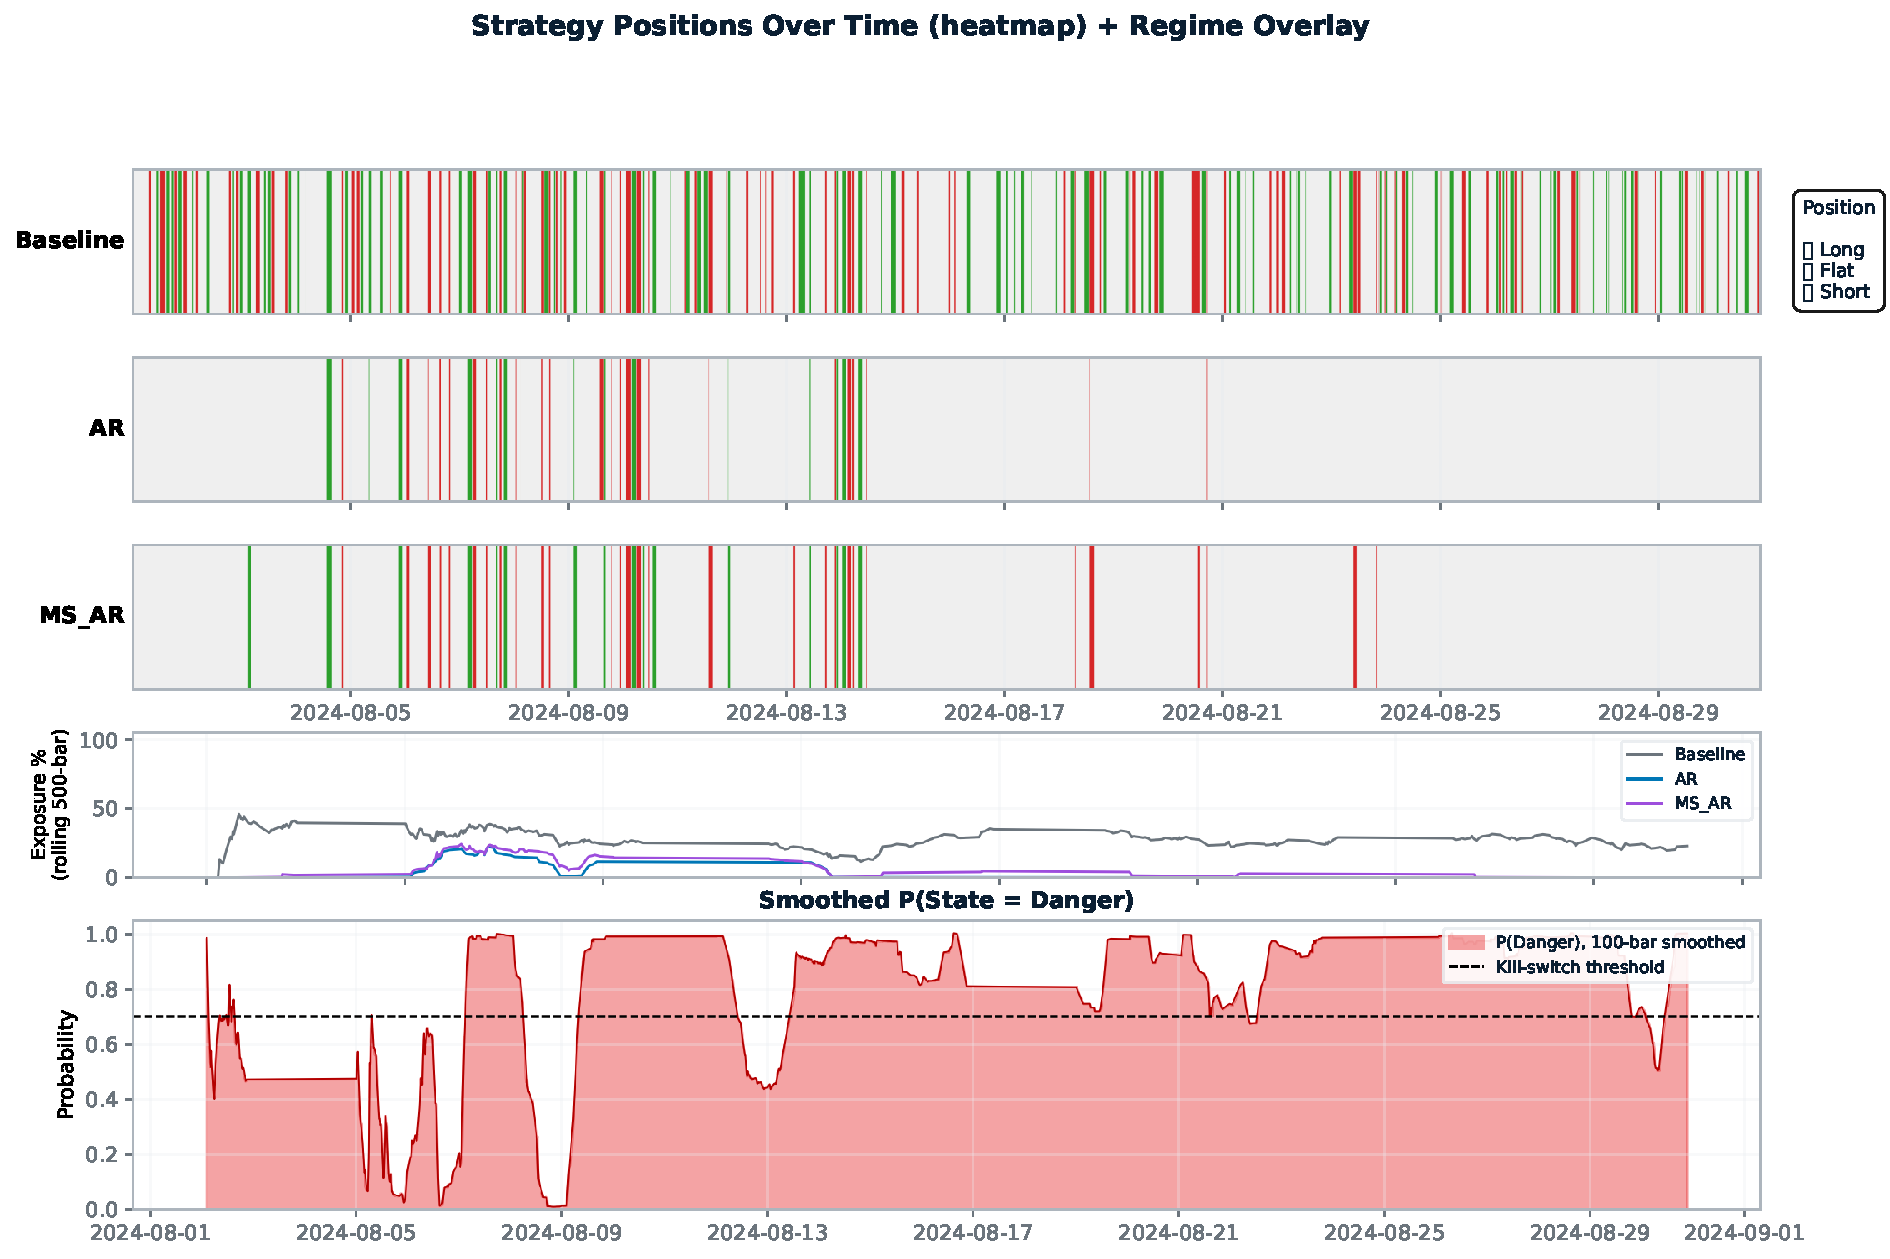
\includegraphics[width=0.7\linewidth, height=0.28\textheight, keepaspectratio]{plots/AUDUSD_NZDUSD_202408_positions_and_regimes.pdf}\\[0.4em]
    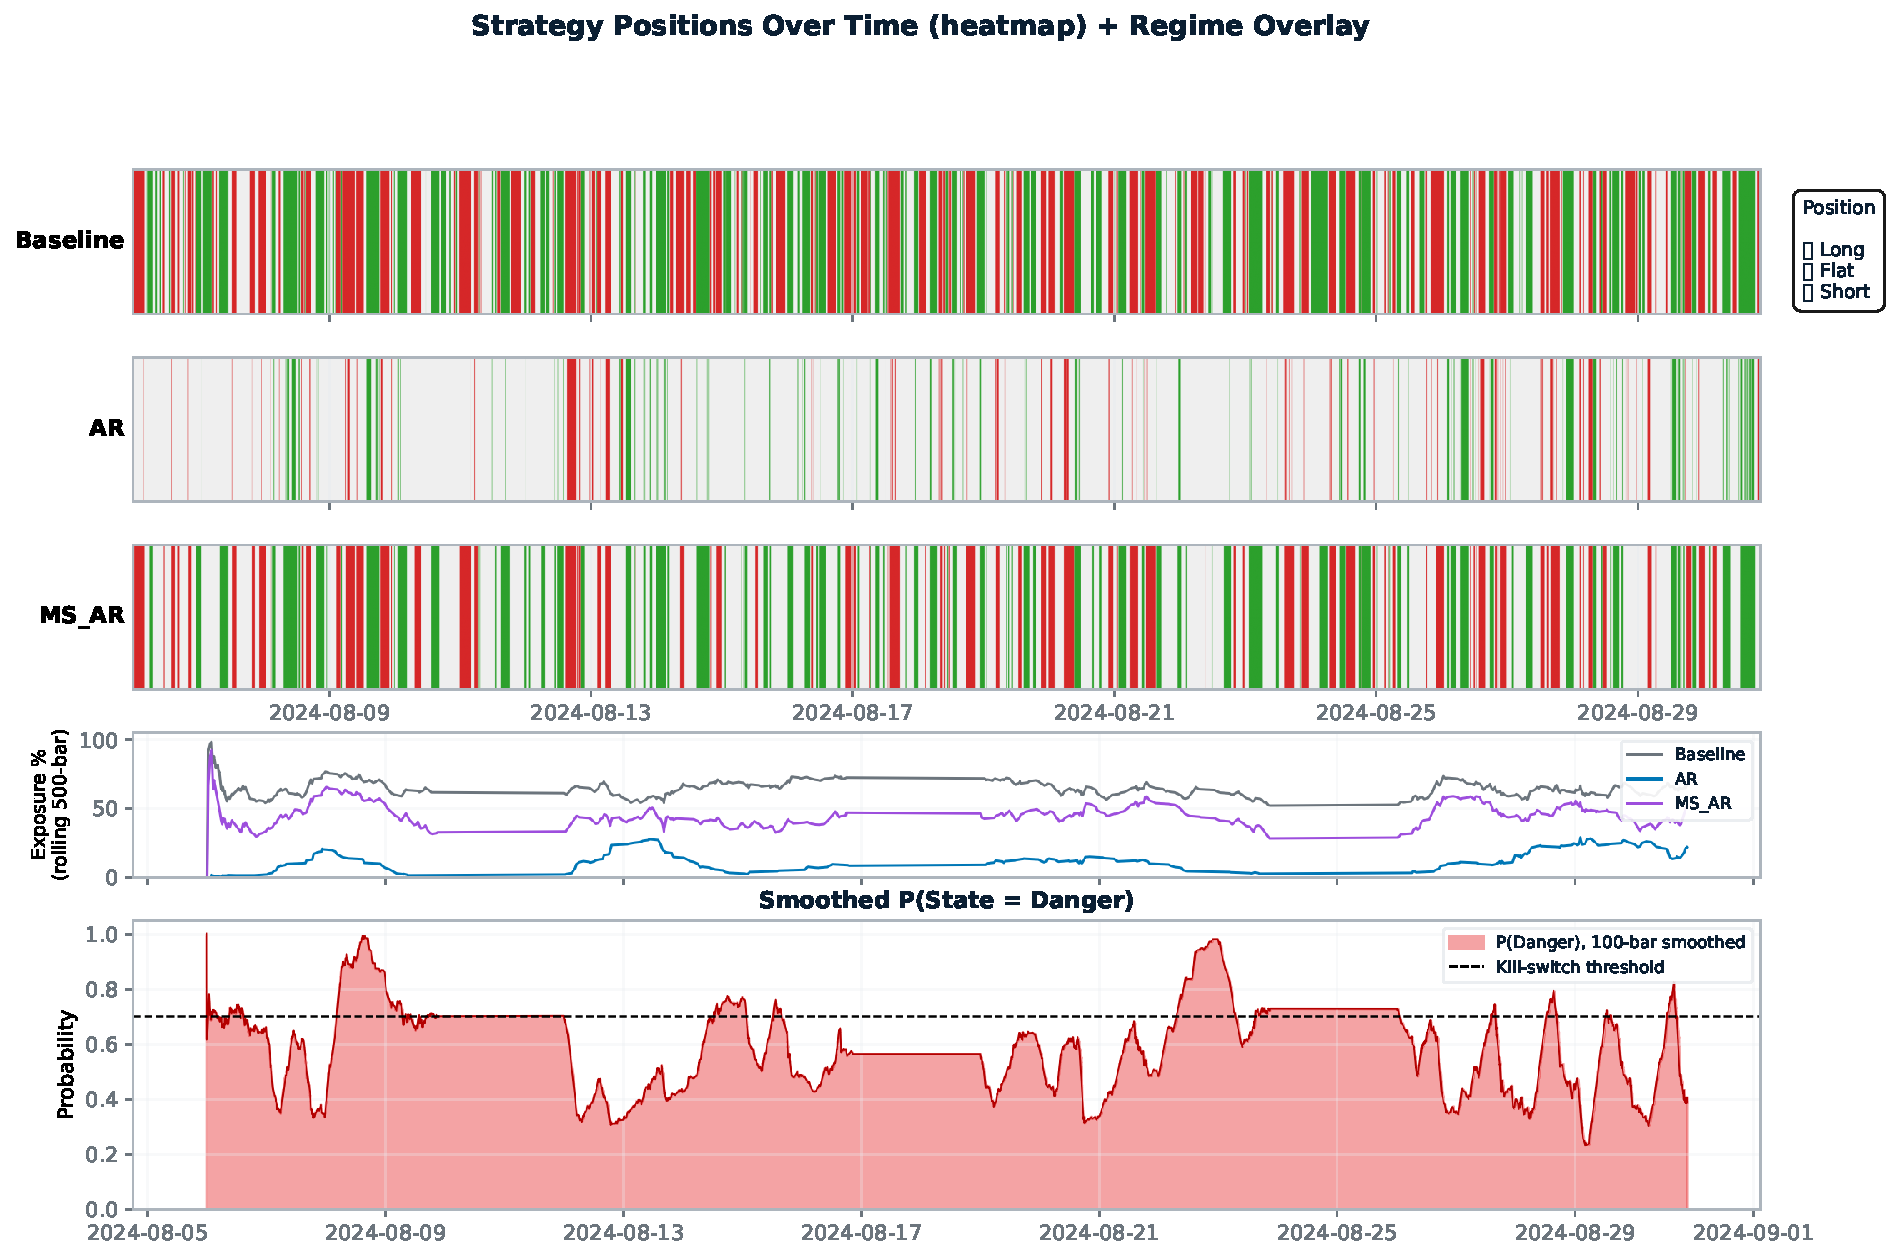
\includegraphics[width=0.7\linewidth, height=0.28\textheight, keepaspectratio]{plots/EURNOK_EURSEK_202408_positions_and_regimes.pdf}\\[0.4em]
    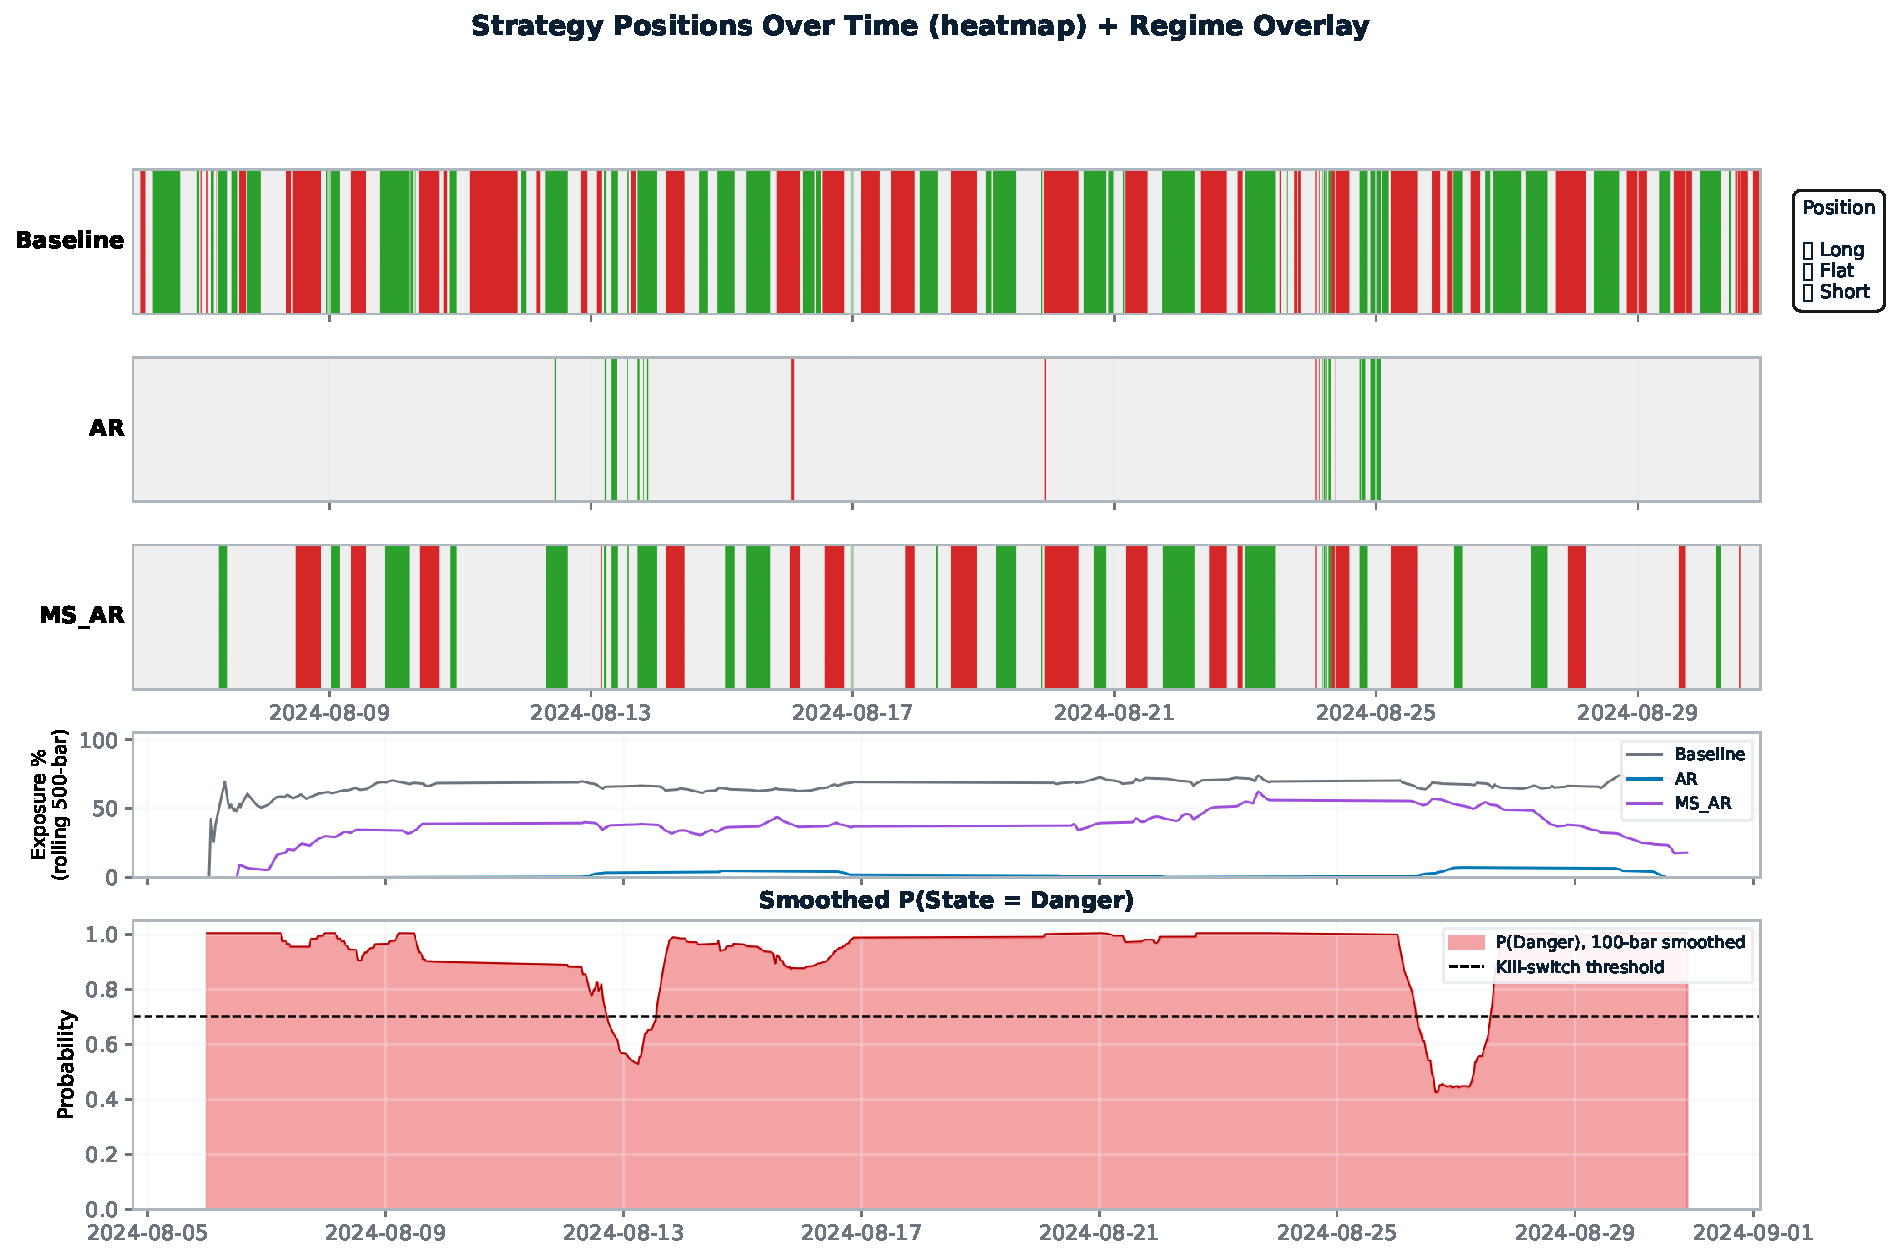
\includegraphics[width=0.7\linewidth, height=0.28\textheight, keepaspectratio]{plots/GBPUSD_EURUSD_202408_positions_and_regimes.pdf}
    \caption{Baseline positions and the HMM-implied regime gate, August 2024. Top: AUD/USD--NZD/USD; middle: EUR/NOK--EUR/SEK; bottom: GBP/USD--EUR/USD.}
    \label{fig:apx-positions-regimes-grid}
\end{figure}
\clearpage

\subsection{Cointegration screener diagnostics}
\label{sec:apx-cointegration-screener}

This appendix reports the cointegration-screening diagnostics for the August 2024 episode of each currency-pair spread. The plots document the pre-trade statistical structure used by the spread engine: whether the two legs share a stable long-run relation, whether the residual spread is plausibly stationary and mean-reverting, and whether the pair is defensible as a relative-value trading candidate. 

\begin{figure}[H]
    \centering
    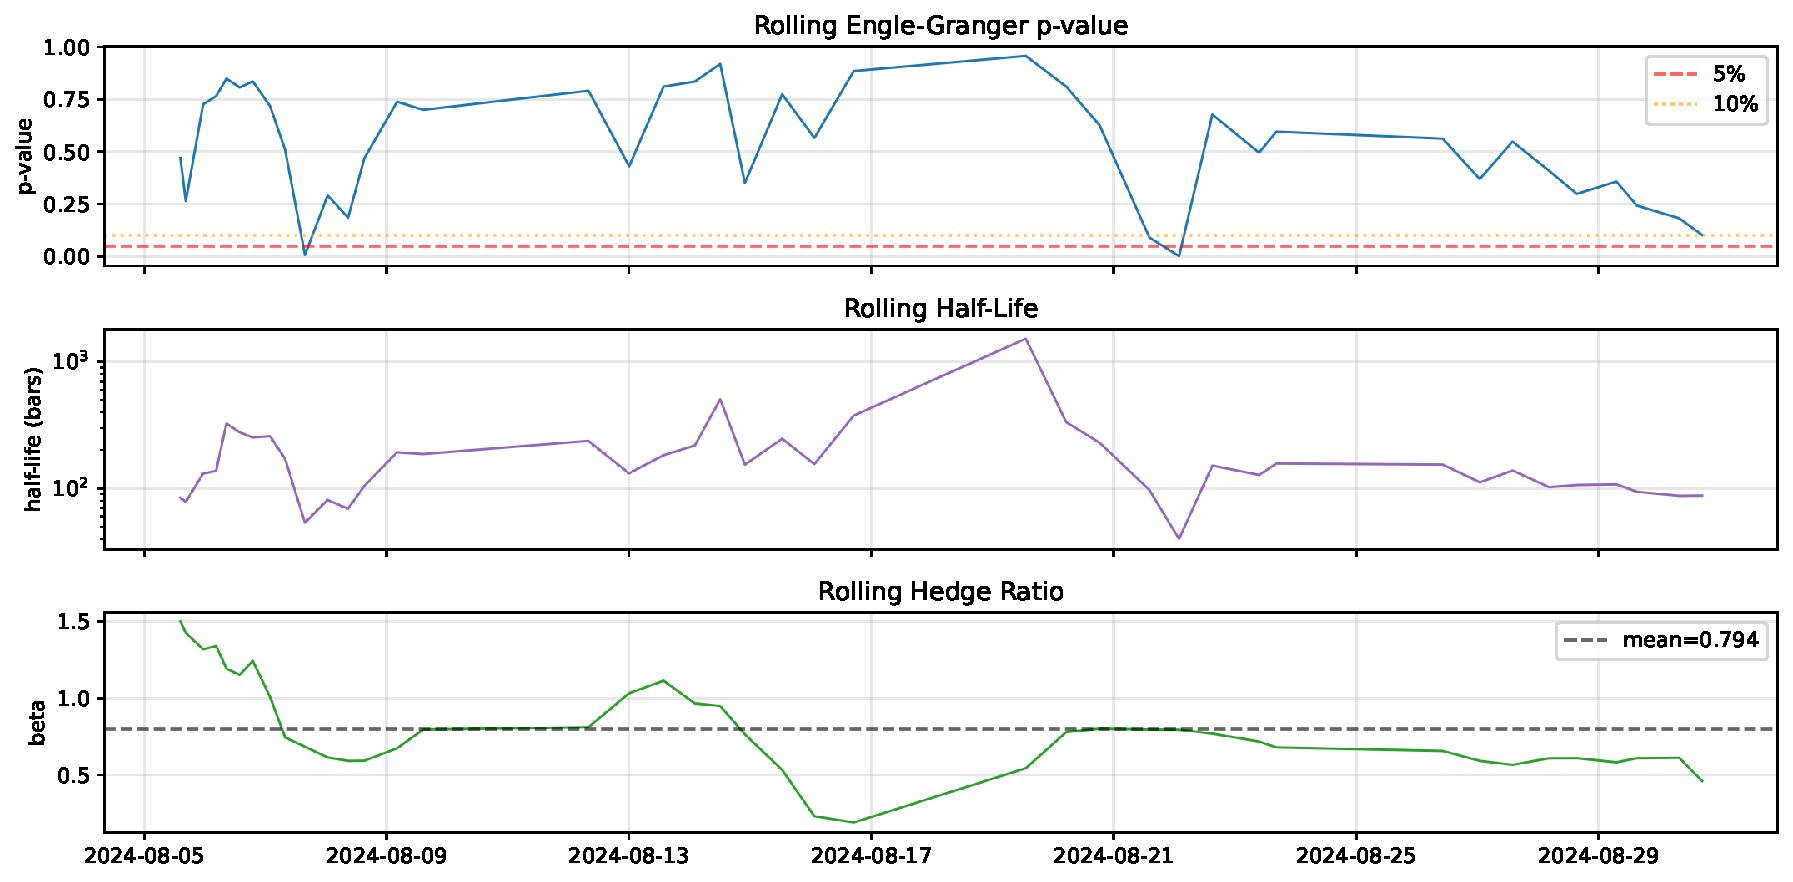
\includegraphics[width=0.7\linewidth]{plots/AUDUSD_NZDUSD_202408_cointegration_screener.pdf}
    \caption{AUD/USD--NZD/USD, August 2024: cointegration screener diagnostics.}
    \label{fig:apx-audnzd-202408-cointegration-screener}
\end{figure}

\begin{figure}[H]
    \centering
    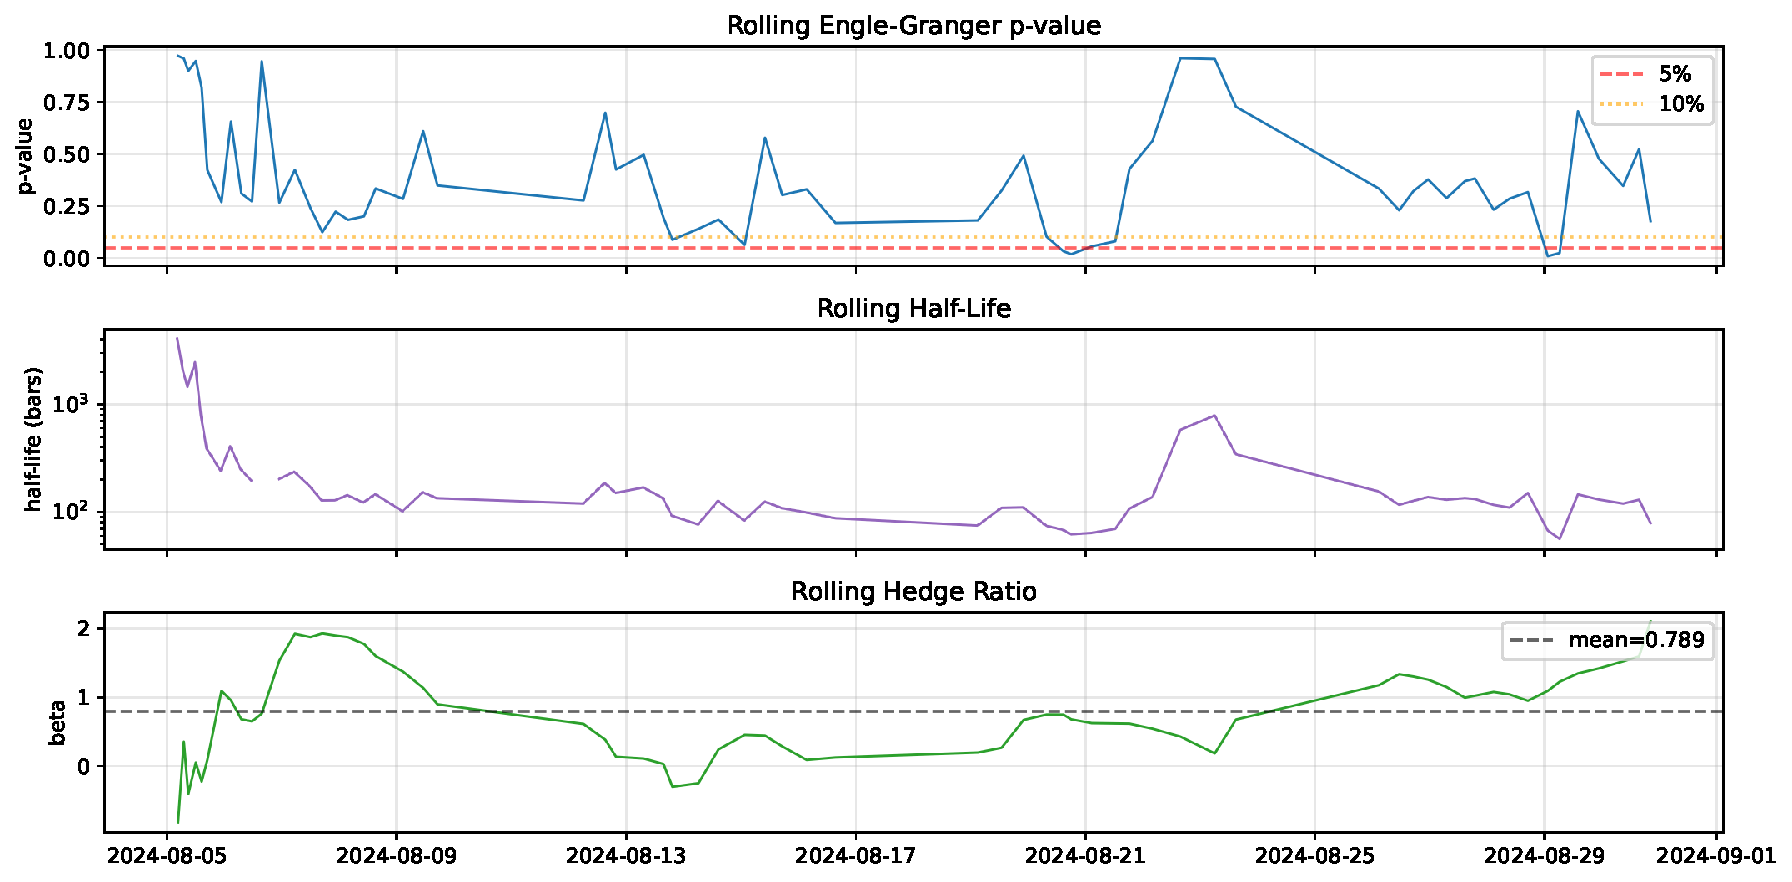
\includegraphics[width=0.7\linewidth]{plots/EURNOK_EURSEK_202408_cointegration_screener.pdf}
    \caption{EUR/NOK--EUR/SEK, August 2024: cointegration screener diagnostics.}
    \label{fig:apx-noksek-202408-cointegration-screener}
\end{figure}

\begin{figure}[H]
    \centering
    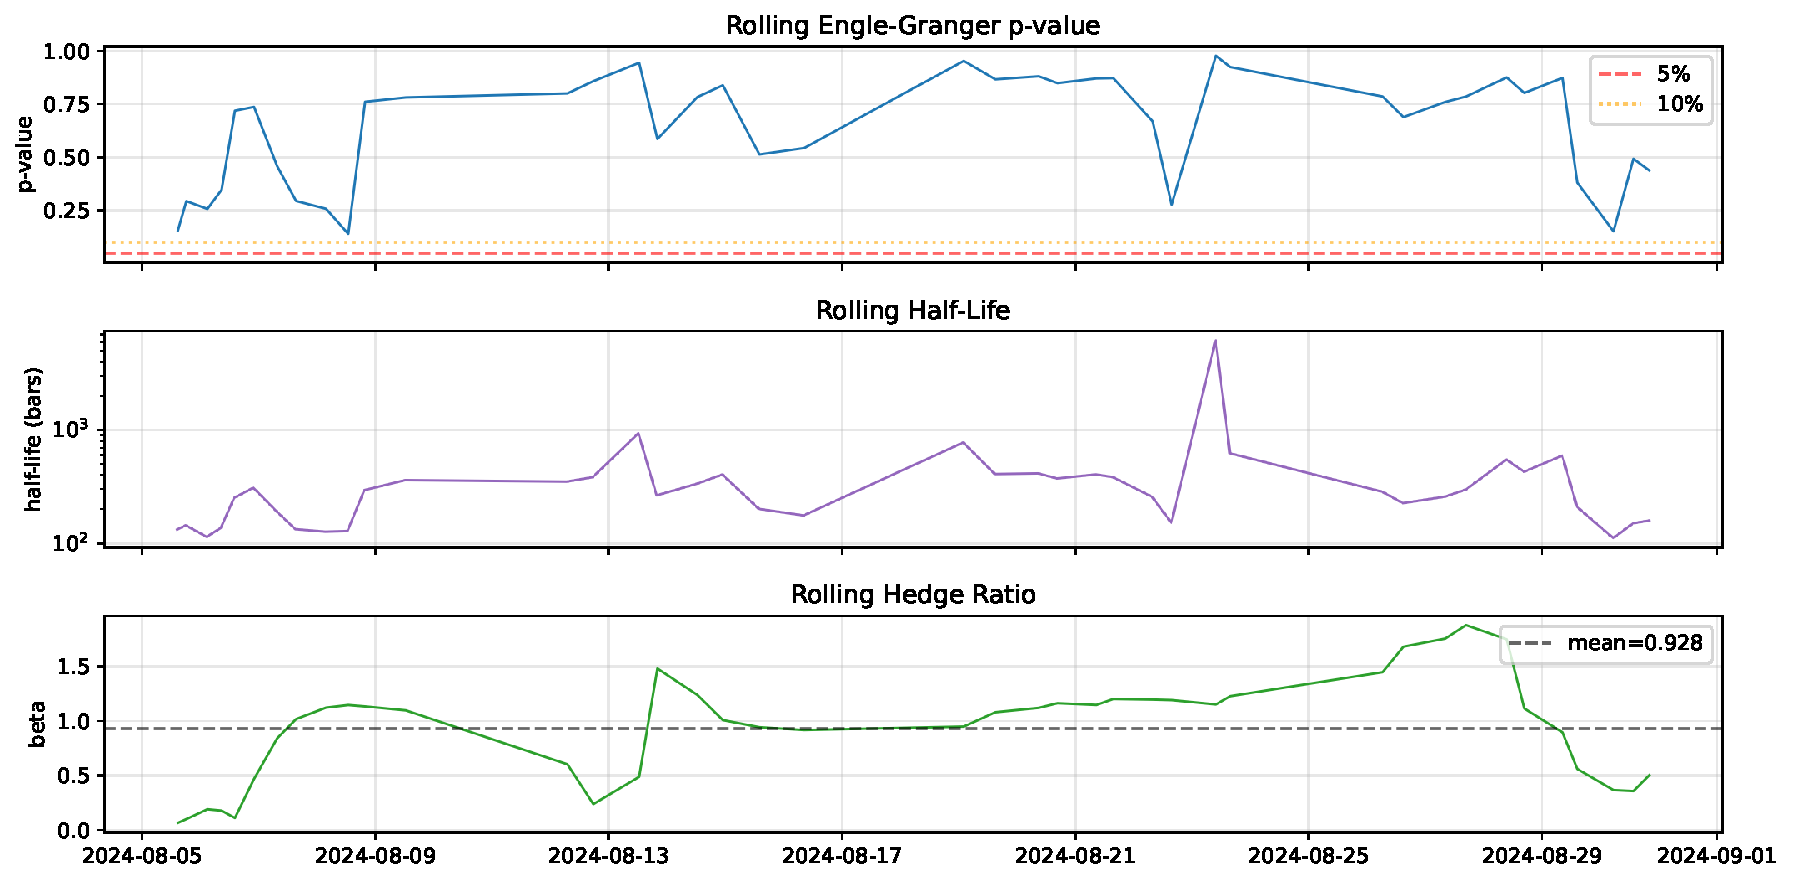
\includegraphics[width=0.7\linewidth]{plots/GBPUSD_EURUSD_202408_cointegration_screener.pdf}
    \caption{GBP/USD--EUR/USD, August 2024: cointegration screener diagnostics.}
    \label{fig:apx-gbpeur-202408-cointegration-screener}
\end{figure}

\clearpage
\section{Period returns}\label{sec:apx-period-returns}

Per-bar period returns for each pair and each monthly episode.

\subsection{AUD/USD--NZD/USD}

\begin{figure}[H]
    \centering
    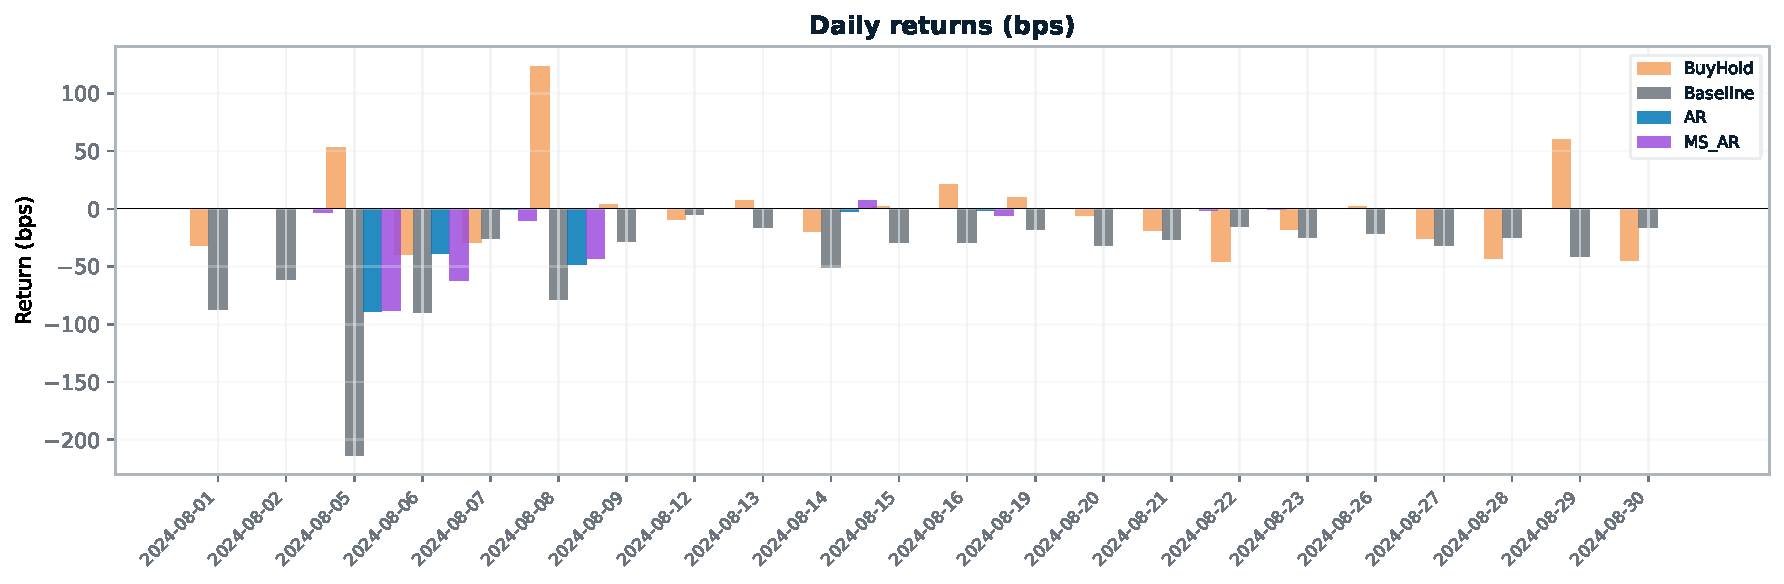
\includegraphics[width=\linewidth]{plots/AUDUSD_NZDUSD_202408_period_returns.pdf}
    \caption{AUD/USD--NZD/USD, August 2024 --- period returns.}
    \label{fig:apx-audnzd-202408-period-returns}
\end{figure}

\begin{figure}[H]
    \centering
    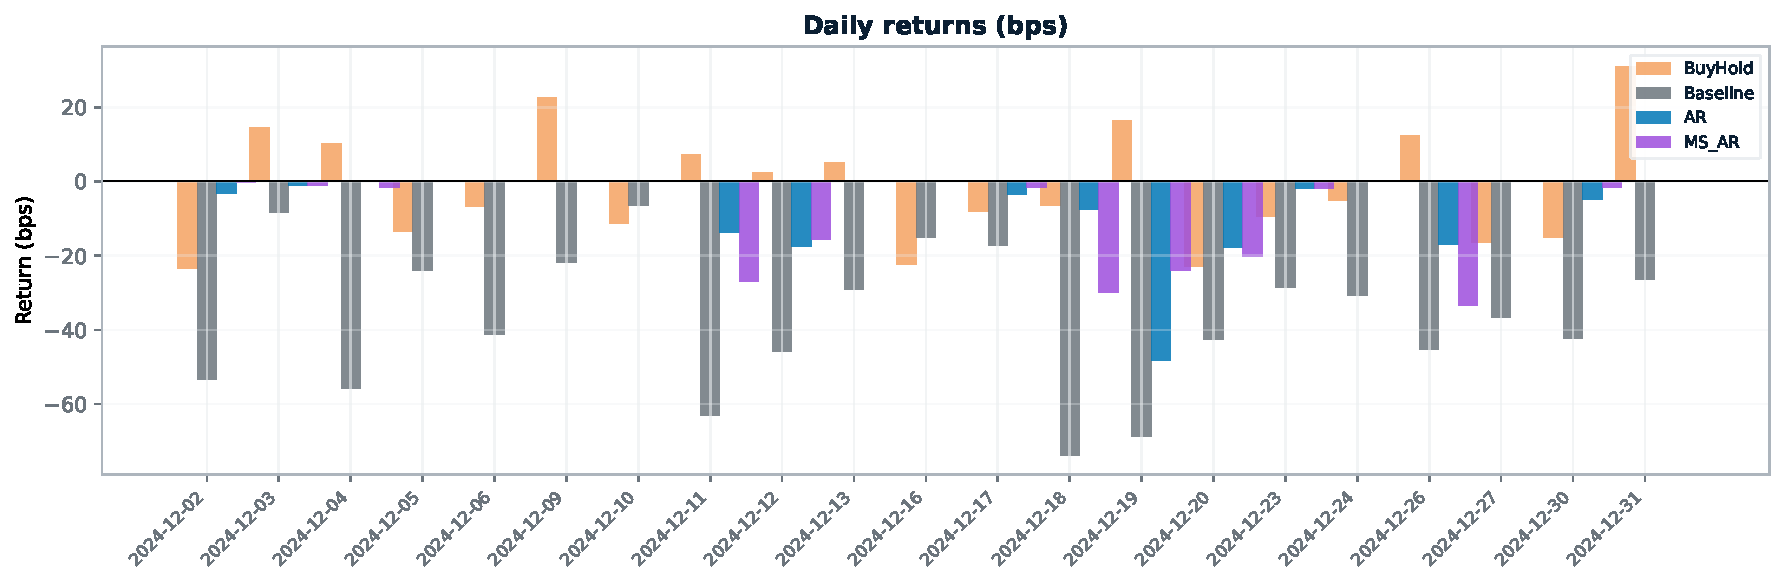
\includegraphics[width=\linewidth]{plots/AUDUSD_NZDUSD_202412_period_returns.pdf}
    \caption{AUD/USD--NZD/USD, December 2024 --- period returns.}
    \label{fig:apx-audnzd-202412-period-returns}
\end{figure}

\begin{figure}[H]
    \centering
    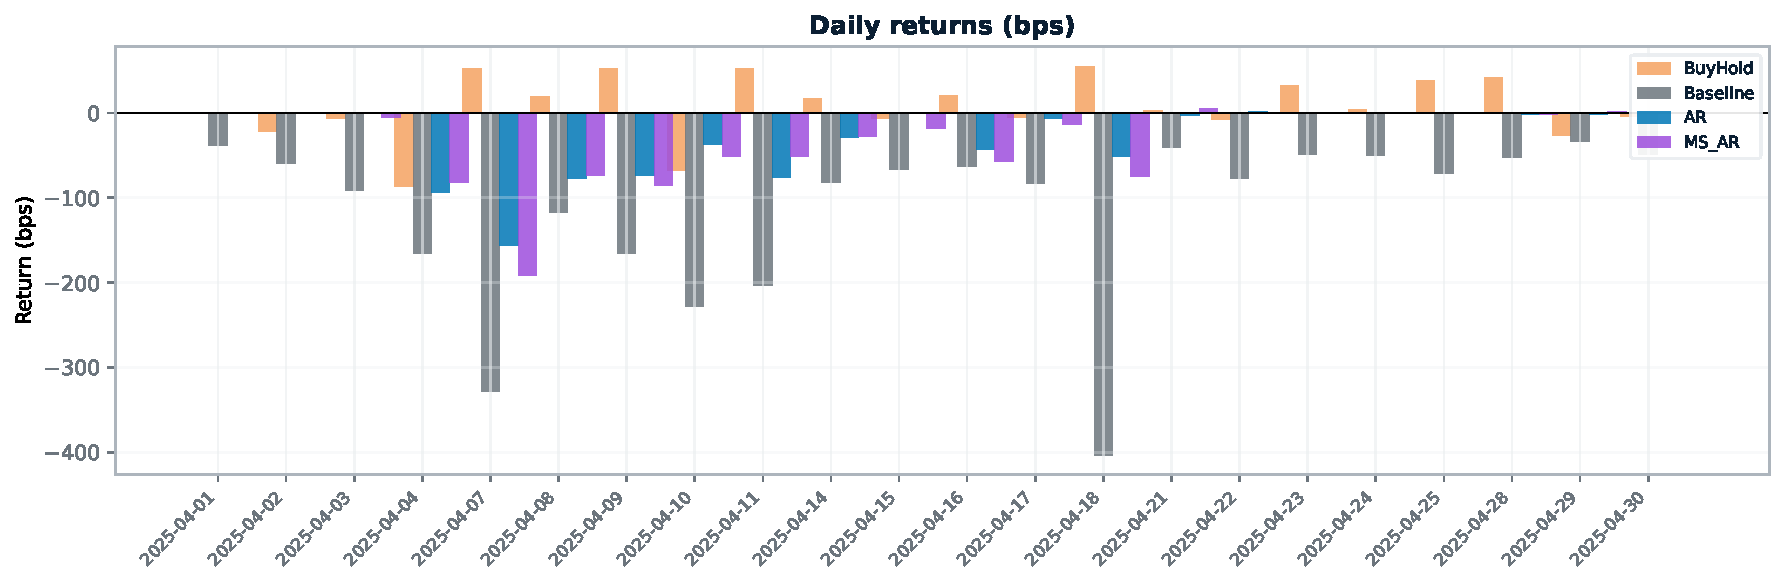
\includegraphics[width=\linewidth]{plots/AUDUSD_NZDUSD_202504_period_returns.pdf}
    \caption{AUD/USD--NZD/USD, April 2025 --- period returns.}
    \label{fig:apx-audnzd-202504-period-returns}
\end{figure}
\clearpage

\subsection{EUR/NOK--EUR/SEK}

\begin{figure}[H]
    \centering
    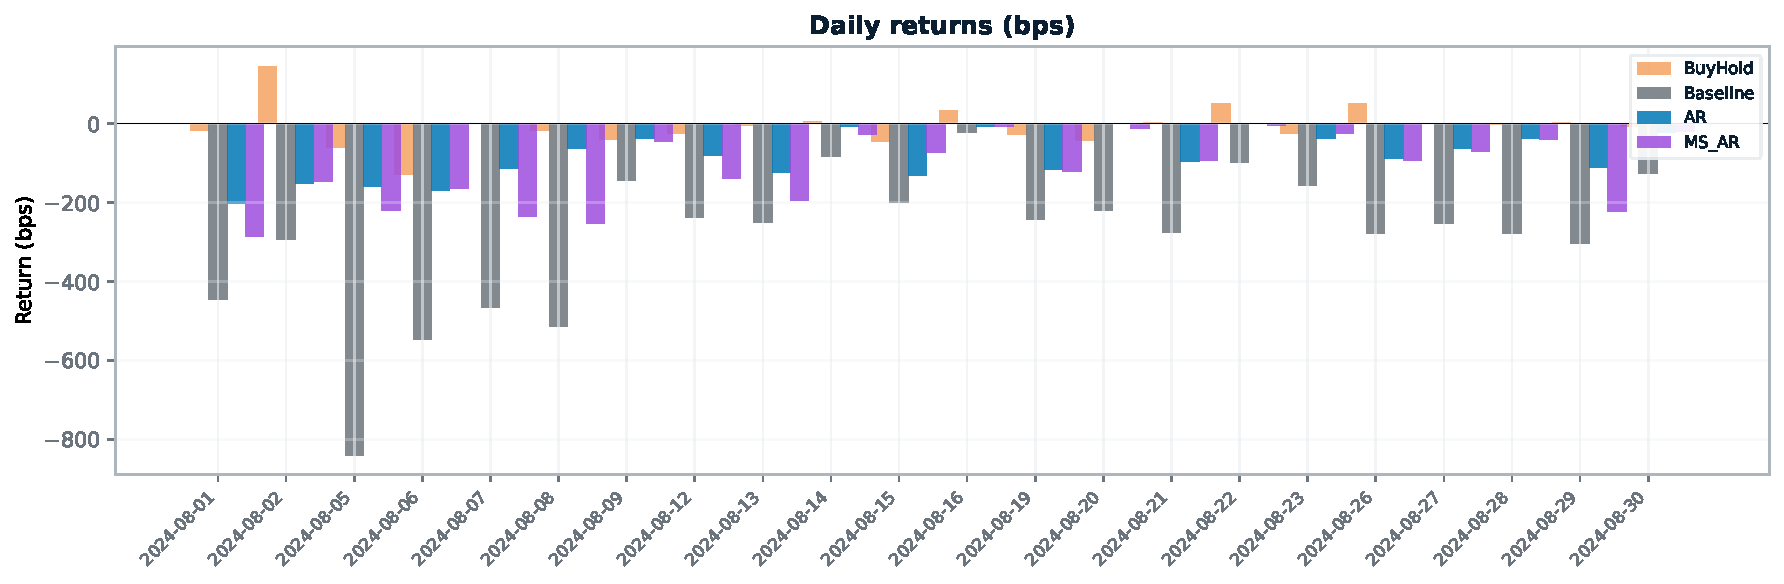
\includegraphics[width=\linewidth]{plots/EURNOK_EURSEK_202408_period_returns.pdf}
    \caption{EUR/NOK--EUR/SEK, August 2024 --- period returns.}
    \label{fig:apx-noksek-202408-period-returns}
\end{figure}

\begin{figure}[H]
    \centering
    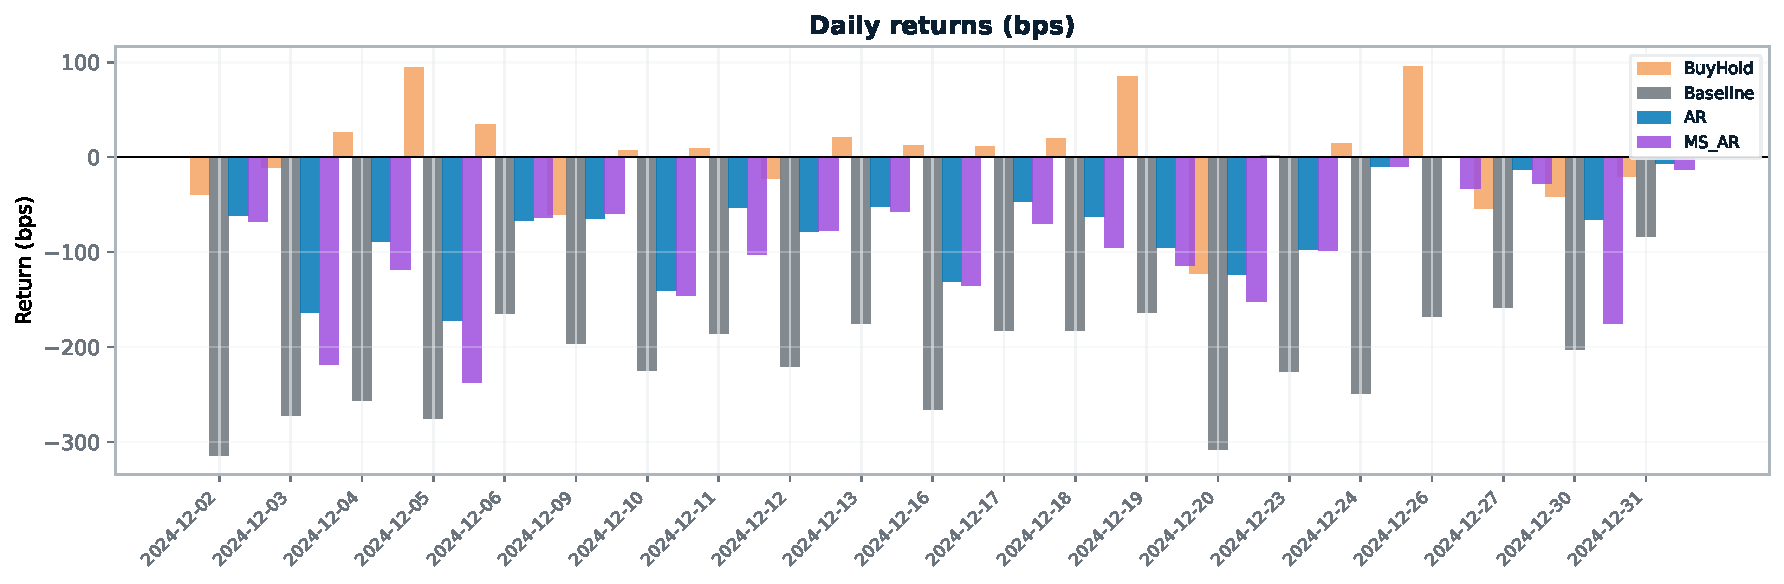
\includegraphics[width=\linewidth]{plots/EURNOK_EURSEK_202412_period_returns.pdf}
    \caption{EUR/NOK--EUR/SEK, December 2024 --- period returns.}
    \label{fig:apx-noksek-202412-period-returns}
\end{figure}

\begin{figure}[H]
    \centering
    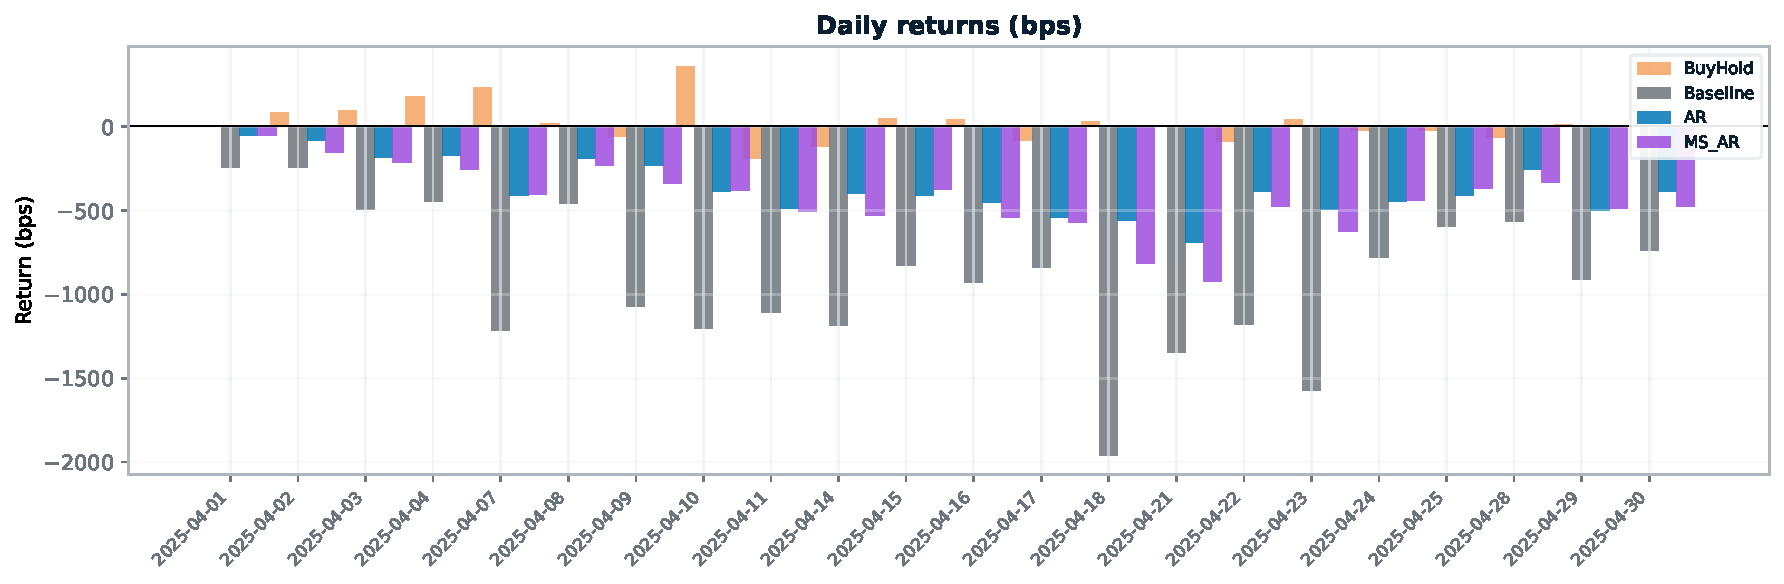
\includegraphics[width=\linewidth]{plots/EURNOK_EURSEK_202504_period_returns.pdf}
    \caption{EUR/NOK--EUR/SEK, April 2025 --- period returns.}
    \label{fig:apx-noksek-202504-period-returns}
\end{figure}
\clearpage

\subsection{GBP/USD--EUR/USD}

\begin{figure}[H]
    \centering
    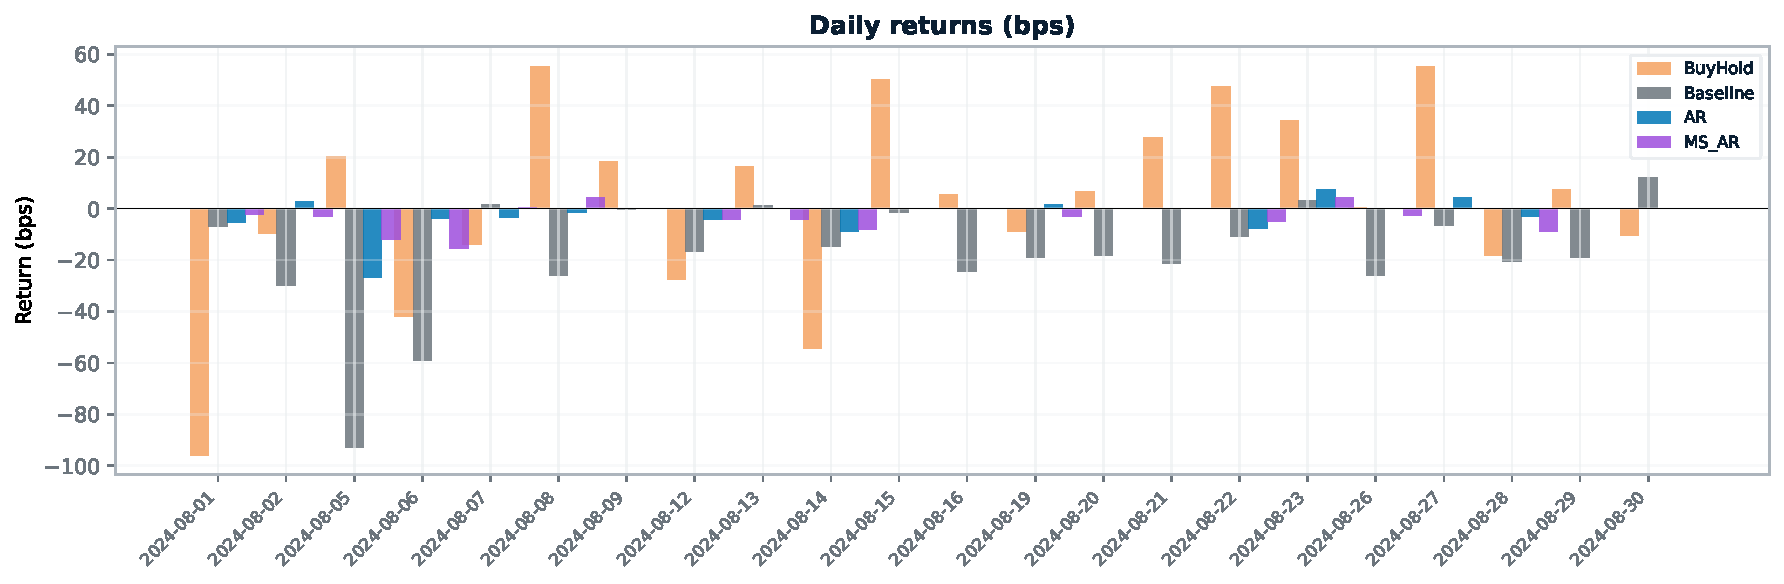
\includegraphics[width=\linewidth]{plots/GBPUSD_EURUSD_202408_period_returns.pdf}
    \caption{GBP/USD--EUR/USD, August 2024 --- period returns.}
    \label{fig:apx-gbpeur-202408-period-returns}
\end{figure}

\begin{figure}[H]
    \centering
    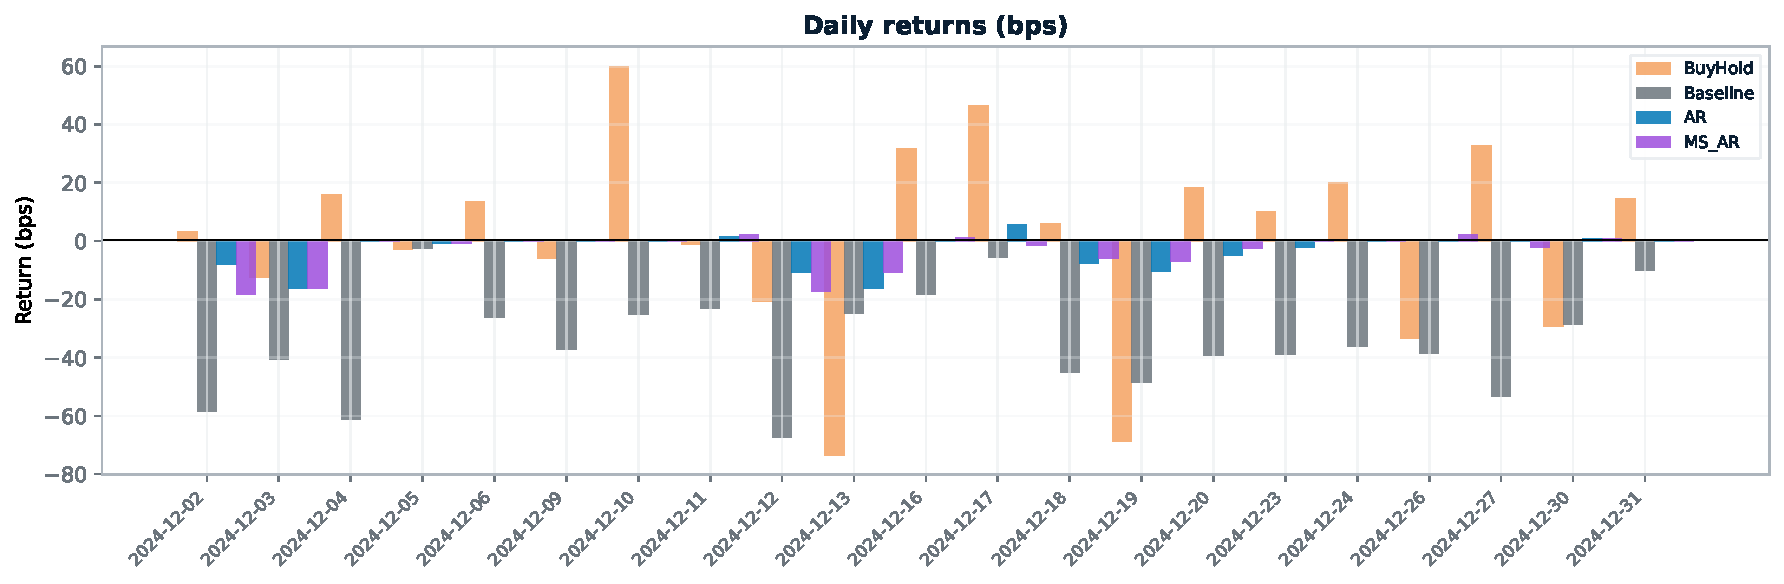
\includegraphics[width=\linewidth]{plots/GBPUSD_EURUSD_202412_period_returns.pdf}
    \caption{GBP/USD--EUR/USD, December 2024 --- period returns.}
    \label{fig:apx-gbpeur-202412-period-returns}
\end{figure}

\begin{figure}[H]
    \centering
    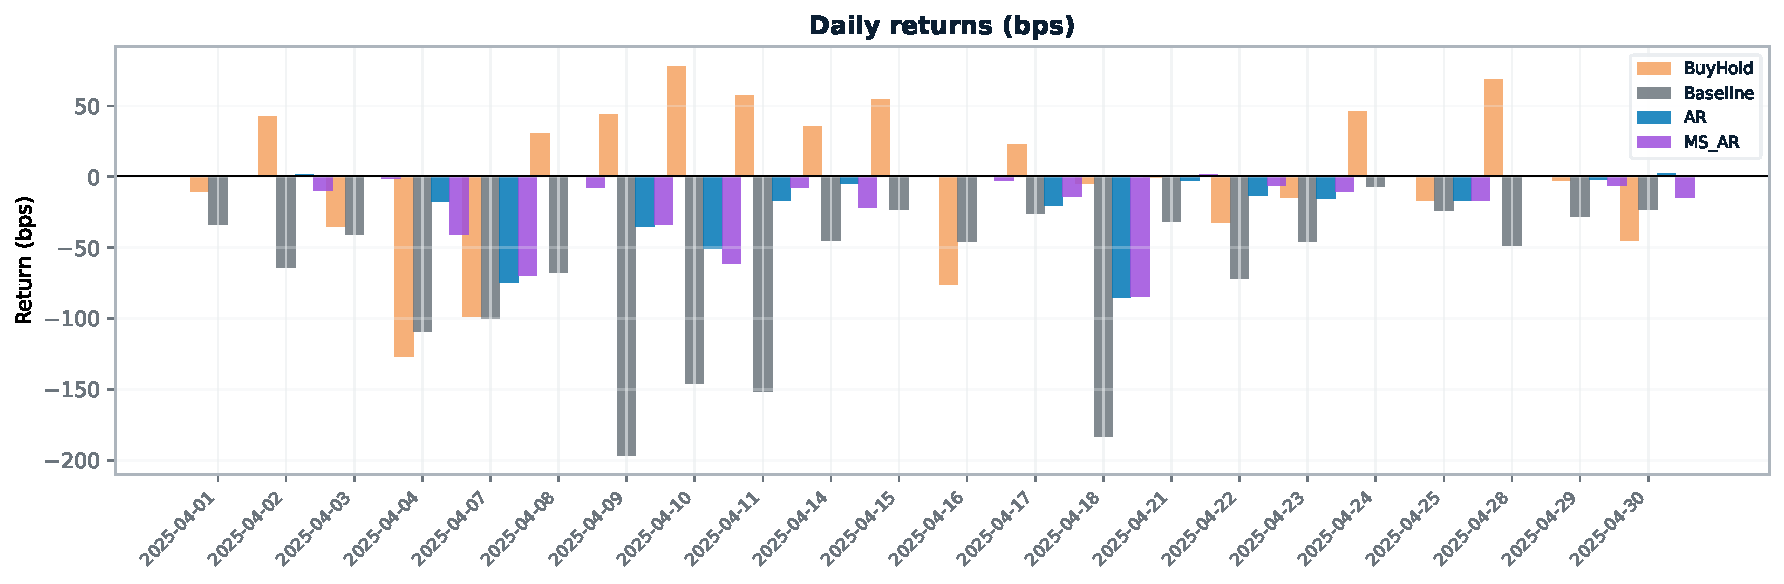
\includegraphics[width=\linewidth]{plots/GBPUSD_EURUSD_202504_period_returns.pdf}
    \caption{GBP/USD--EUR/USD, April 2025 --- period returns.}
    \label{fig:apx-gbpeur-202504-period-returns}
\end{figure}
\clearpage


\subsection{AUDUSD-NZDUSD}

\begin{figure}[H]
    \centering
    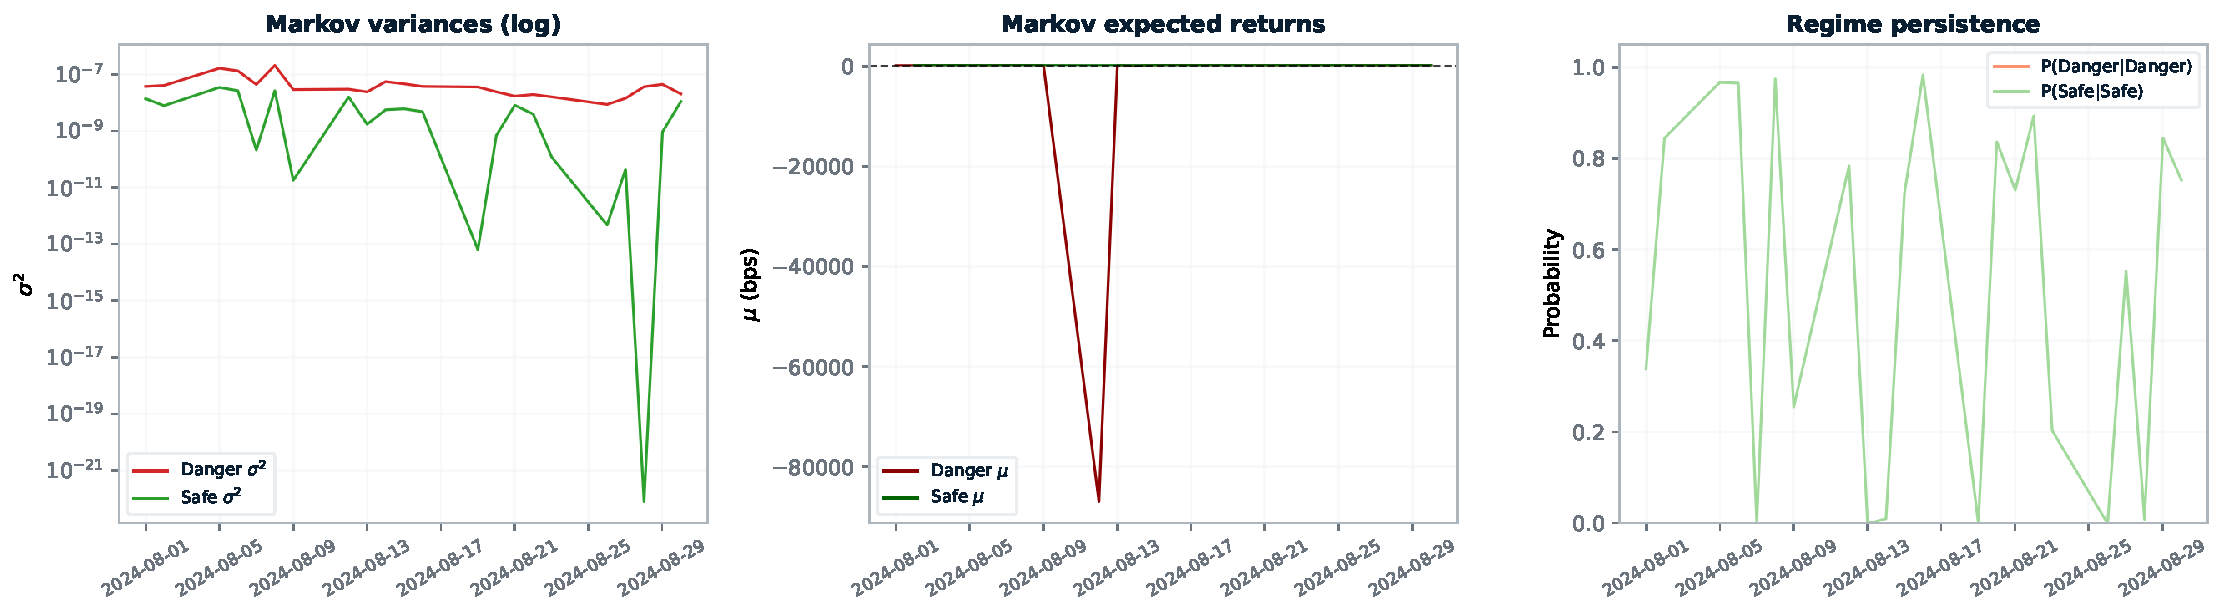
\includegraphics[width=\linewidth]{plots/AUDUSD_NZDUSD_202408_markov_dynamics.pdf}
    \caption{Caption}
    \label{fig:placeholder}
\end{figure}

\begin{figure}[H]
    \centering
    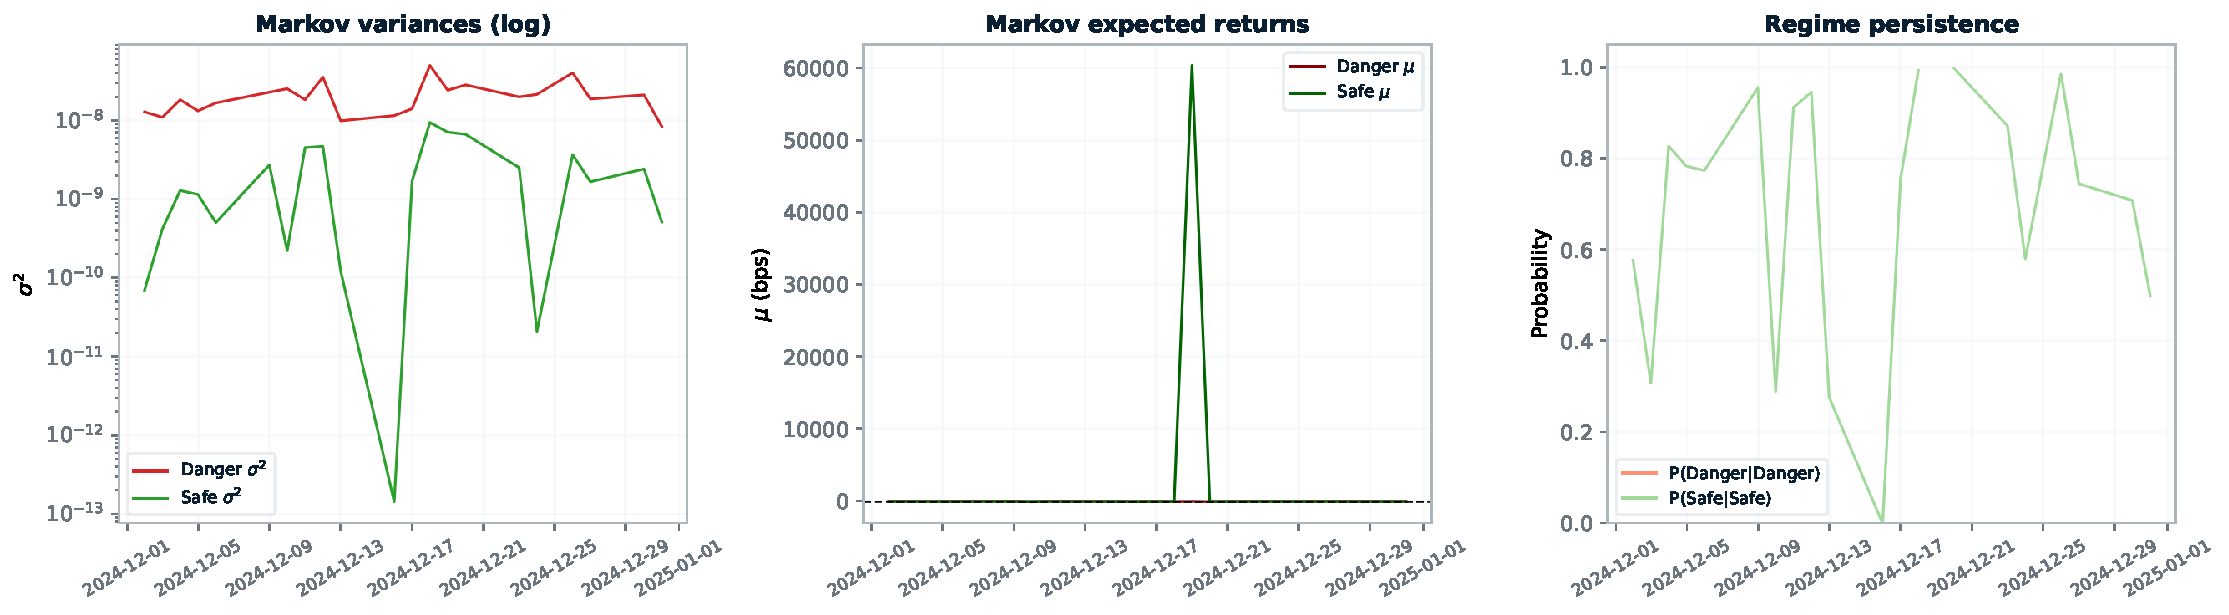
\includegraphics[width=\linewidth]{plots/AUDUSD_NZDUSD_202412_markov_dynamics.pdf}
    \caption{Caption}
    \label{fig:placeholder}
\end{figure}

\begin{figure}[H]
    \centering
    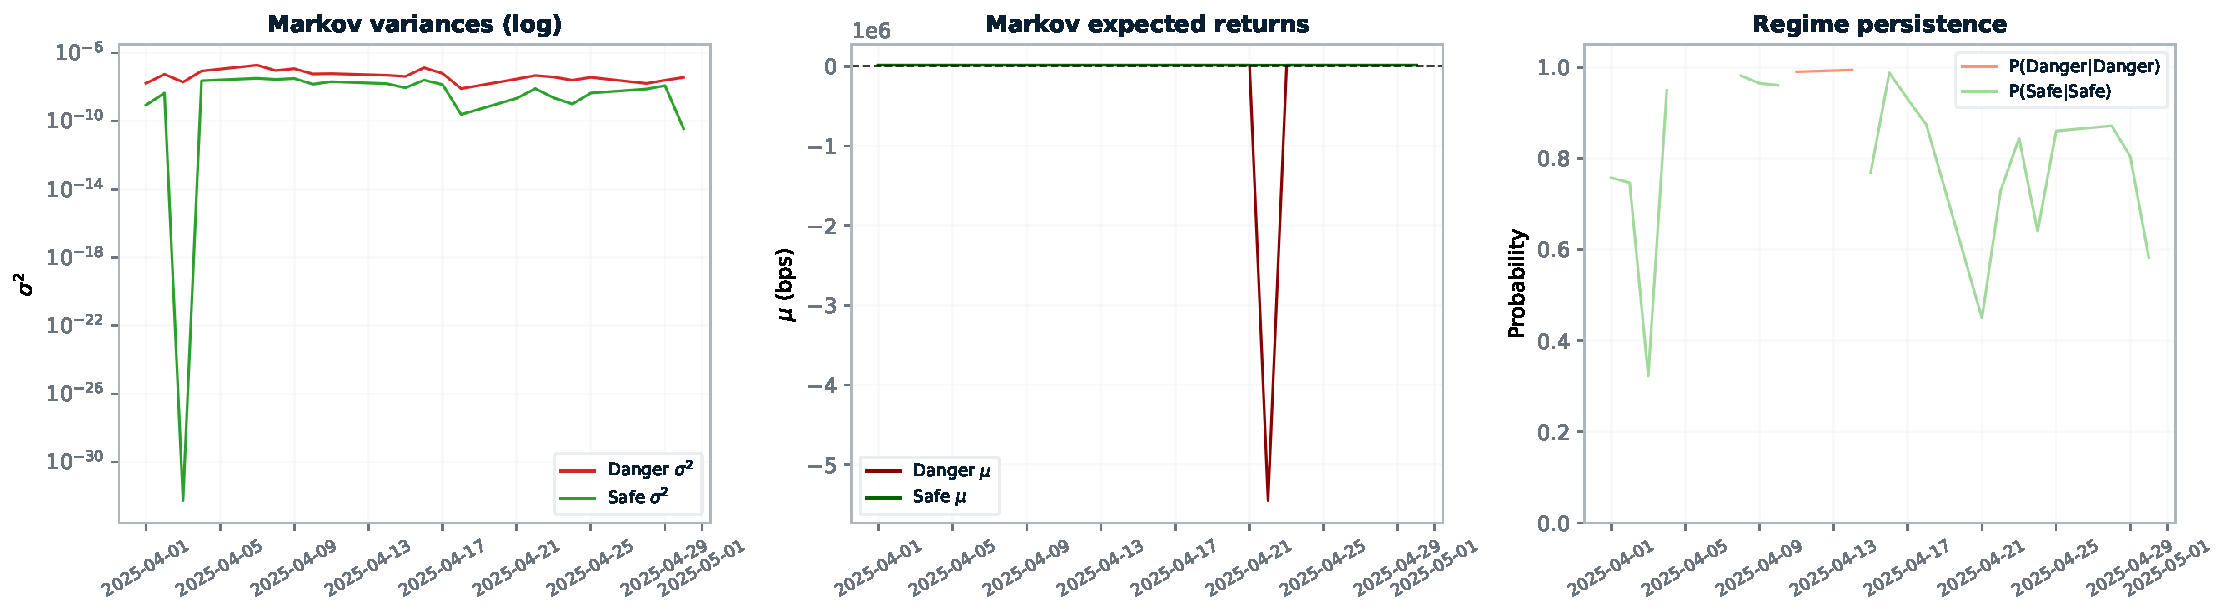
\includegraphics[width=\linewidth]{plots/AUDUSD_NZDUSD_202504_markov_dynamics.pdf}
    \caption{Caption}
    \label{fig:placeholder}
\end{figure}


\subsection{EURNOK-EURSEK}



\subsection{GBPUSD-EURUSD}



\section{Drawdowns}\label{sec:apx-drawdown}

Strategy drawdown curves $D_t = (V_t^{\star} - V_t)/V_t^{\star}$ per pair and per month.

\subsection{AUD/USD--NZD/USD}

\begin{figure}[H]
    \centering
    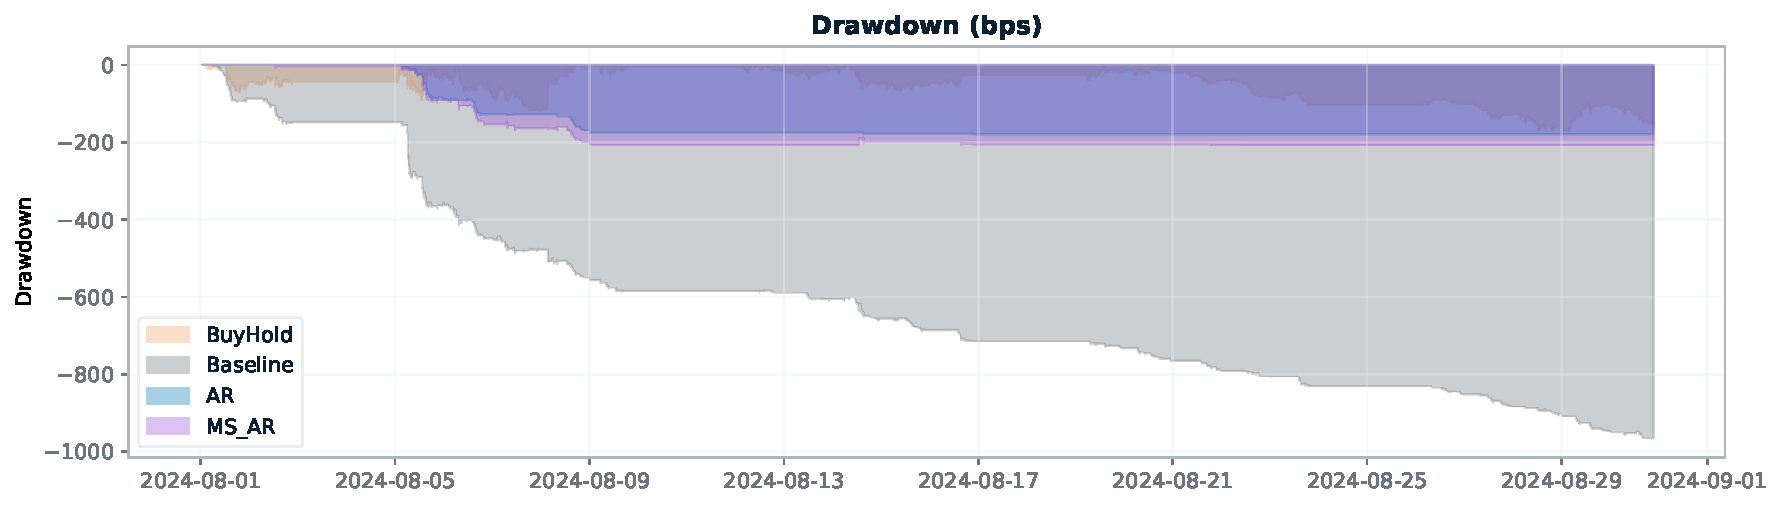
\includegraphics[width=\linewidth]{plots/AUDUSD_NZDUSD_202408_drawdown.pdf}
    \caption{AUD/USD--NZD/USD, August 2024 --- strategy drawdowns.}
    \label{fig:apx-audnzd-202408-drawdown}
\end{figure}

\begin{figure}[H]
    \centering
    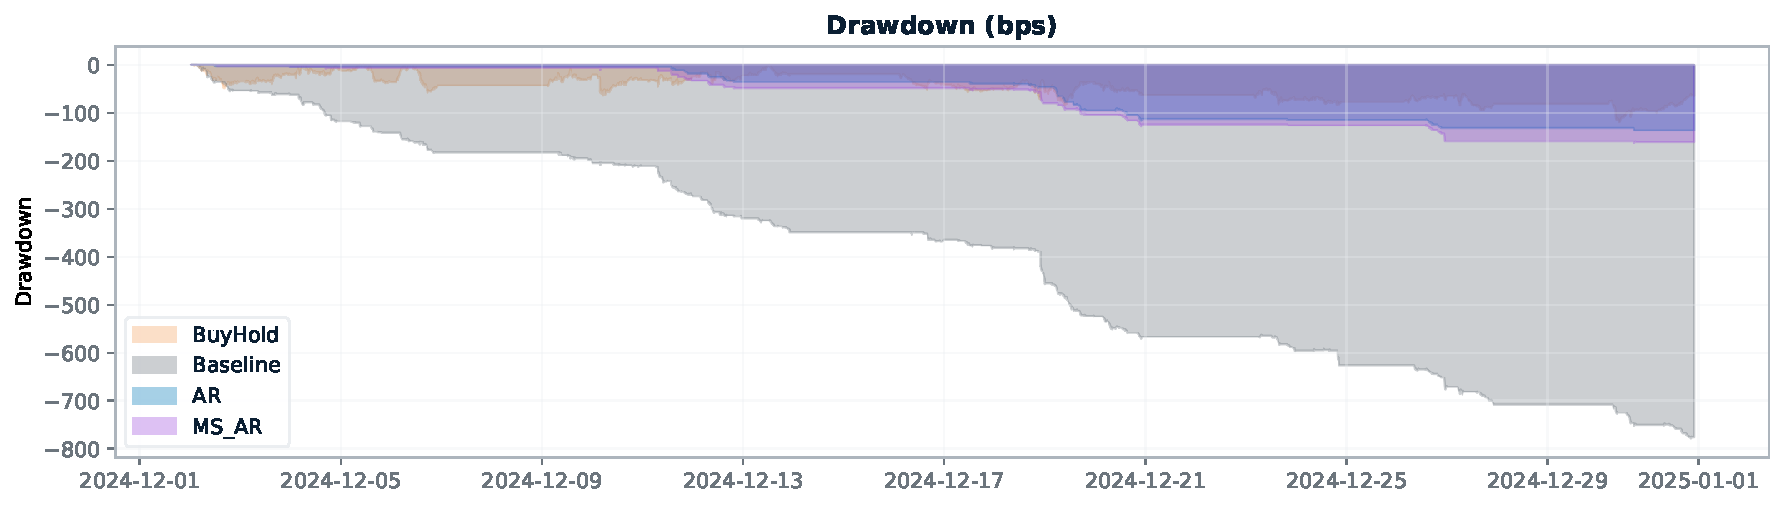
\includegraphics[width=\linewidth]{plots/AUDUSD_NZDUSD_202412_drawdown.pdf}
    \caption{AUD/USD--NZD/USD, December 2024 --- strategy drawdowns.}
    \label{fig:apx-audnzd-202412-drawdown}
\end{figure}

\begin{figure}[H]
    \centering
    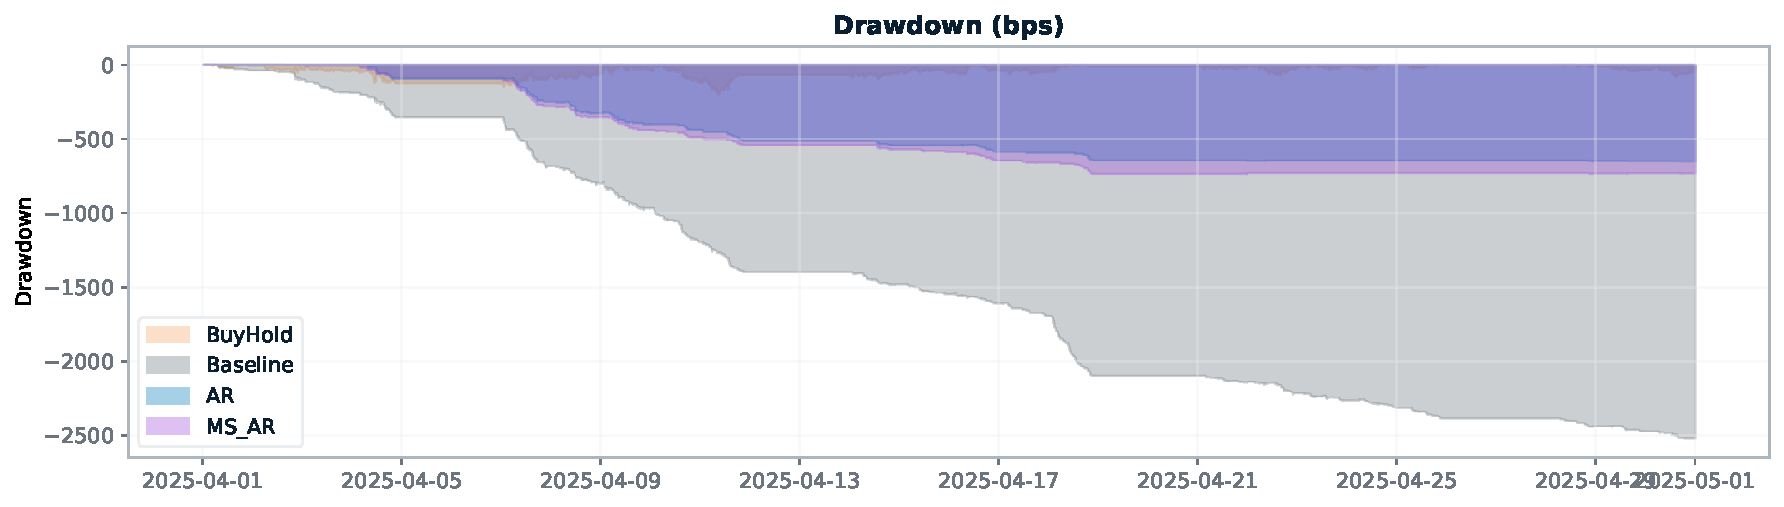
\includegraphics[width=\linewidth]{plots/AUDUSD_NZDUSD_202504_drawdown.pdf}
    \caption{AUD/USD--NZD/USD, April 2025 --- strategy drawdowns.}
    \label{fig:apx-audnzd-202504-drawdown}
\end{figure}
\clearpage

\subsection{EUR/NOK--EUR/SEK}

\begin{figure}[H]
    \centering
    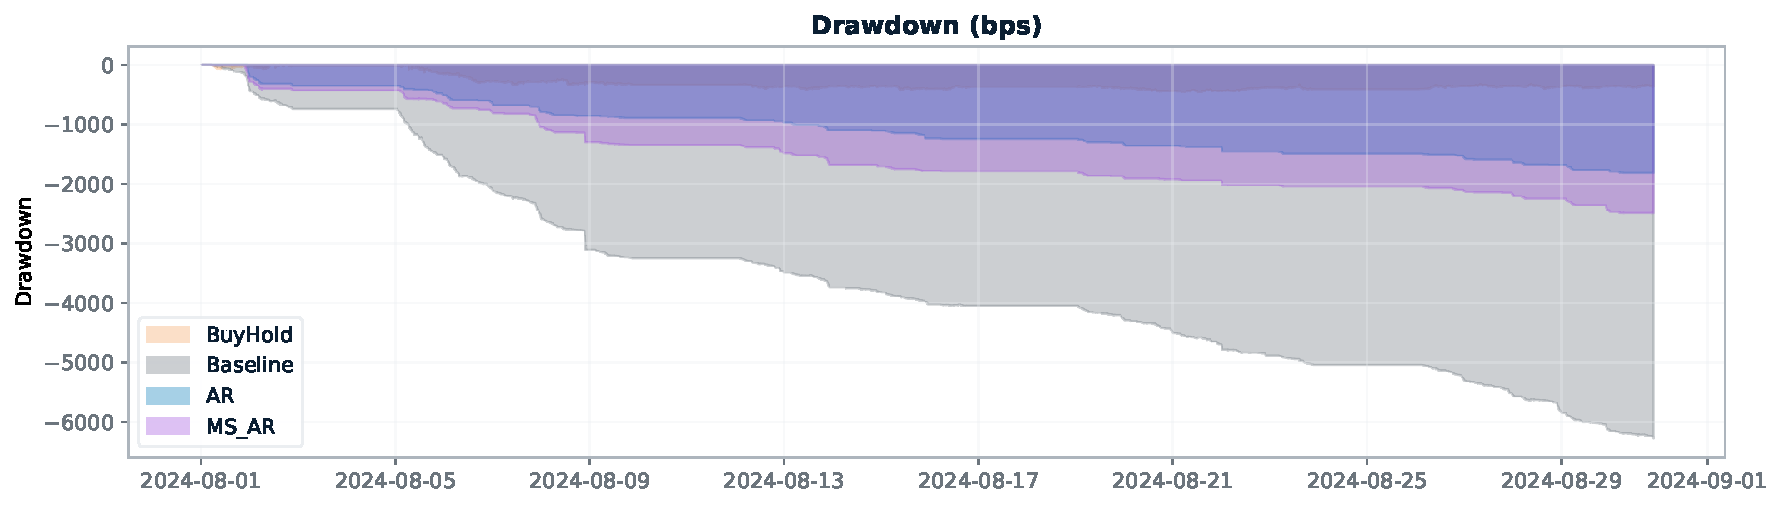
\includegraphics[width=\linewidth]{plots/EURNOK_EURSEK_202408_drawdown.pdf}
    \caption{EUR/NOK--EUR/SEK, August 2024 --- strategy drawdowns.}
    \label{fig:apx-noksek-202408-drawdown}
\end{figure}

\begin{figure}[H]
    \centering
    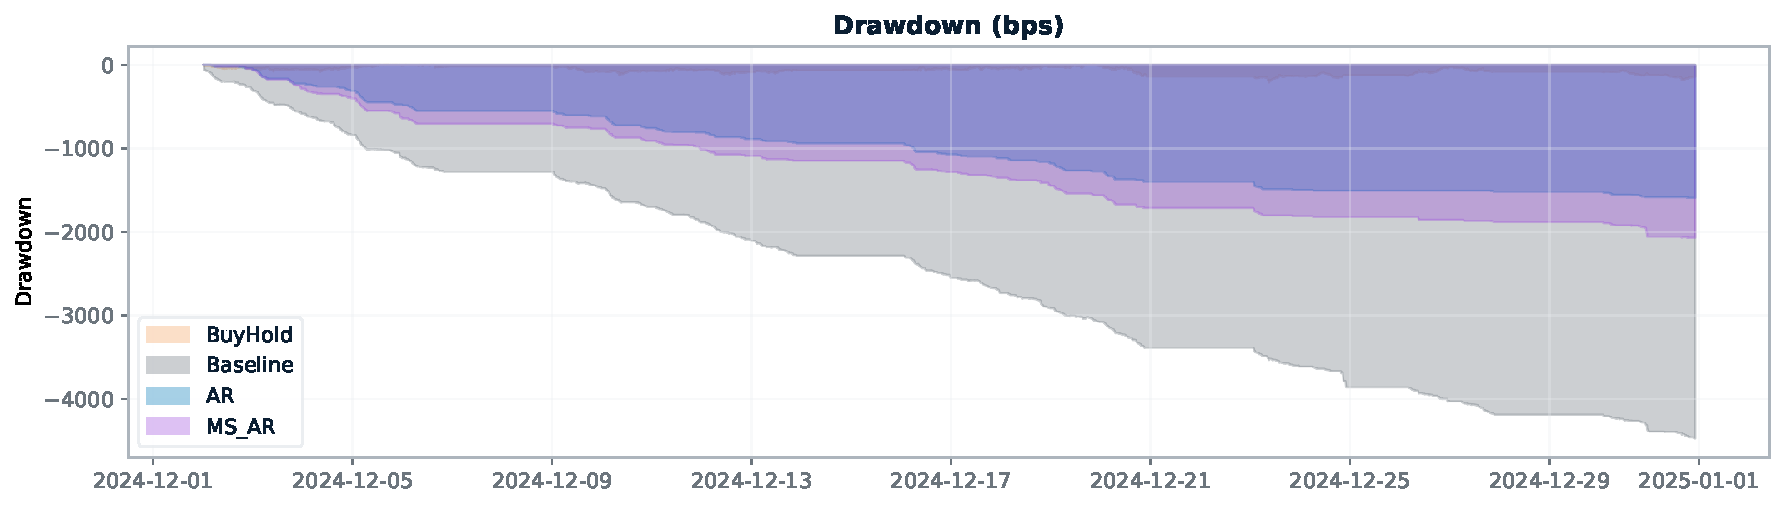
\includegraphics[width=\linewidth]{plots/EURNOK_EURSEK_202412_drawdown.pdf}
    \caption{EUR/NOK--EUR/SEK, December 2024 --- strategy drawdowns.}
    \label{fig:apx-noksek-202412-drawdown}
\end{figure}

\begin{figure}[H]
    \centering
    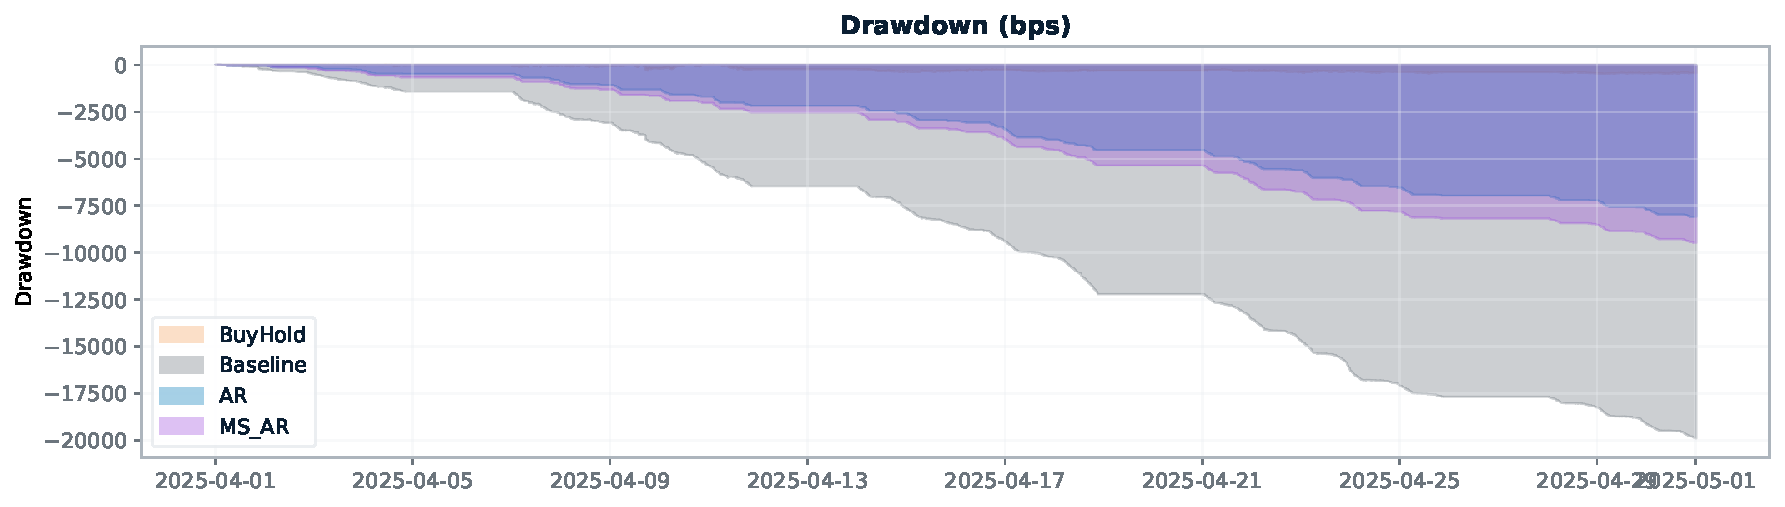
\includegraphics[width=\linewidth]{plots/EURNOK_EURSEK_202504_drawdown.pdf}
    \caption{EUR/NOK--EUR/SEK, April 2025 --- strategy drawdowns.}
    \label{fig:apx-noksek-202504-drawdown}
\end{figure}
\clearpage

\subsection{GBP/USD--EUR/USD}

\begin{figure}[H]
    \centering
    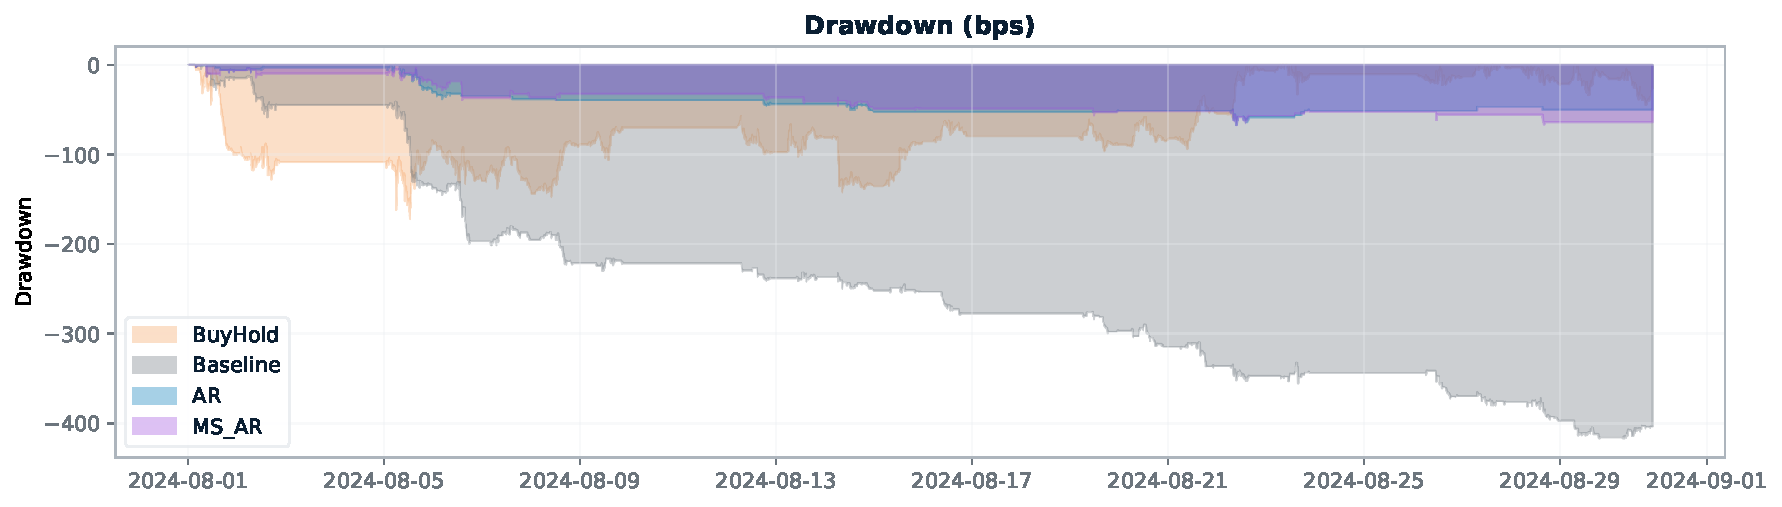
\includegraphics[width=\linewidth]{plots/GBPUSD_EURUSD_202408_drawdown.pdf}
    \caption{GBP/USD--EUR/USD, August 2024 --- strategy drawdowns.}
    \label{fig:apx-gbpeur-202408-drawdown}
\end{figure}

\begin{figure}[H]
    \centering
    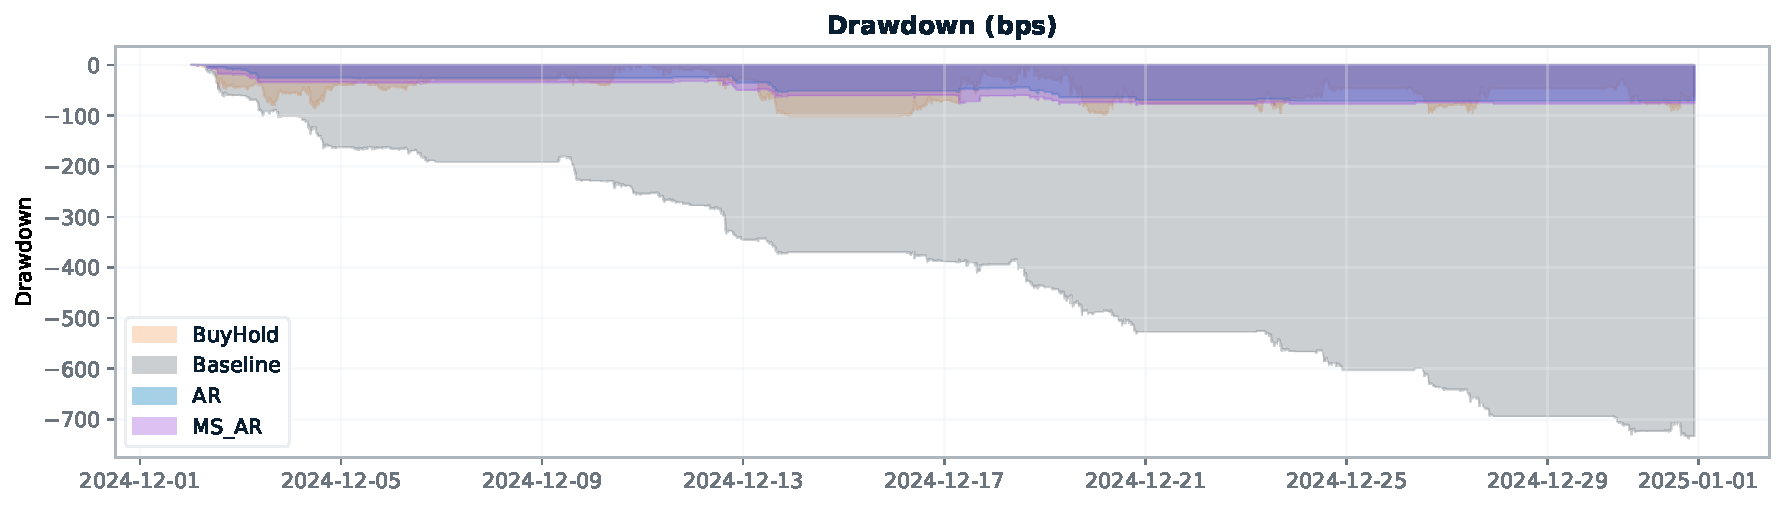
\includegraphics[width=\linewidth]{plots/GBPUSD_EURUSD_202412_drawdown.pdf}
    \caption{GBP/USD--EUR/USD, December 2024 --- strategy drawdowns.}
    \label{fig:apx-gbpeur-202412-drawdown}
\end{figure}

\begin{figure}[H]
    \centering
    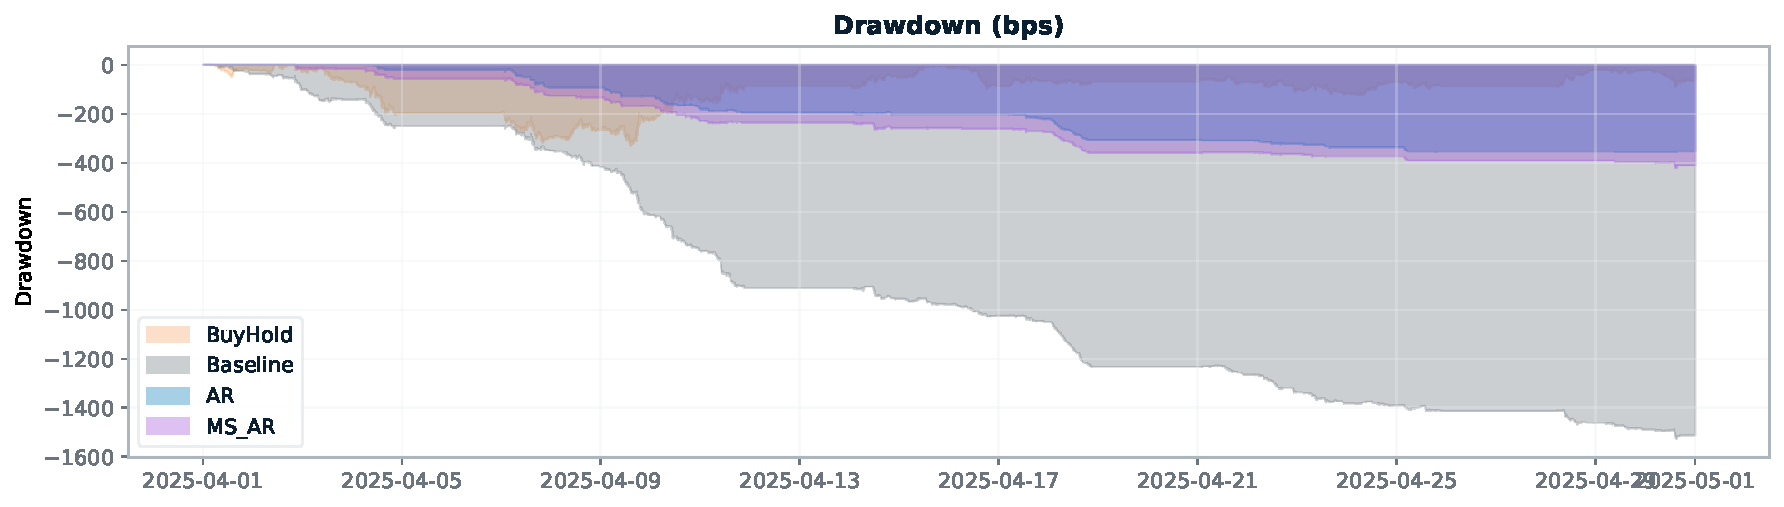
\includegraphics[width=\linewidth]{plots/GBPUSD_EURUSD_202504_drawdown.pdf}
    \caption{GBP/USD--EUR/USD, April 2025 --- strategy drawdowns.}
    \label{fig:apx-gbpeur-202504-drawdown}
\end{figure}
\clearpage

\newpage

\begin{table}[H]
\centering
\caption{\textbf{Daily AUD/USD--NZD/USD strategy summaries.}}
\label{tab:app_gbpeur_daily_stacked}
\vspace{-0.8em}

\scriptsize
\setlength{\tabcolsep}{1.7pt}
\renewcommand{\arraystretch}{0.78}

\begin{tabular*}{\textwidth}{@{\extracolsep{\fill}} lllll}
\toprule
Date & BH & BL & AR & MS \\
\midrule

\multicolumn{5}{@{}l}{\textbf{August 2024}}\\
08-01 & L, NF; -31.34 & F/M, 11RT; -87.51 & F/M, NF; +0.00 & F/M, NF; +0.00 \\
08-02 & L, NF; +0.48 & F/M, 13RT; -61.19 & F/M, NF; +0.00 & F/M, 1RT; -3.14 \\
08-05 & L, NF; +53.17 & F/M, 25RT; -213.20 & F/M, 16RT; -88.65 & F/M, 14RT; -87.77 \\
08-06 & L, NF; -39.24 & F/M, 19RT; -90.09 & F/M, 11RT; -38.79 & F/M, 12RT; -61.67 \\
08-07 & L, NF; -29.49 & F/M, 12RT; -25.74 & F/M, 2RT; -0.34 & F/M, 2RT; -10.24 \\
08-08 & L, NF; +123.49 & F/M, 10RT; -78.58 & F/M, 7RT; -47.92 & F/M, 9RT; -42.99 \\
08-09 & L, NF; +4.02 & F/M, 4RT; -28.14 & F/M, NF; +0.00 & F/M, NF; +0.00 \\
08-12 & L, NF; -9.05 & F/M, 3RT; -4.94 & F/M, NF; +0.00 & F/M, NF; +0.00 \\
08-13 & L, NF; +7.00 & F/M, 5RT; -16.18 & F/M, NF; +0.00 & F/M, NF; +0.00 \\
08-14 & L, NF; -19.86 & F/M, 8RT; -50.83 & F/M, 1RT; -2.11 & F/M, 2RT; +7.35 \\
08-15 & L, NF; +2.26 & F/M, 7RT; -29.29 & F/M, NF; +0.00 & F/M, NF; +0.00 \\
08-16 & L, NF; +21.36 & F/M, 3RT; -29.23 & F/M, 1RT; -1.48 & F/M, 2RT; -6.00 \\
08-19 & L, NF; +9.80 & F/M, 5RT; -18.18 & F/M, NF; +0.00 & F/M, NF; +0.00 \\
08-20 & L, NF; -5.42 & F/M, 6RT; -32.01 & F/M, NF; +0.00 & F/M, NF; +0.00 \\
08-21 & L, NF; -18.57 & F/M, 4RT; -26.17 & F/M, NF; +0.00 & F/M, 1RT; -1.36 \\
08-22 & L, NF; -45.36 & F/M, 9RT; -14.86 & F/M, NF; +0.00 & F/M, 1RT; -0.25 \\
08-23 & L, NF; -18.31 & F/M, 5RT; -24.71 & F/M, NF; +0.00 & F/M, NF; +0.00 \\
08-26 & L, NF; +2.29 & F/M, 9RT; -21.43 & F/M, NF; +0.00 & F/M, NF; +0.00 \\
08-27 & L, NF; -25.98 & F/M, 6RT; -31.83 & F/M, NF; +0.00 & F/M, NF; +0.00 \\
08-28 & L, NF; -42.90 & F/M, 7RT; -24.97 & F/M, NF; +0.00 & F/M, NF; +0.00 \\
08-29 & L, NF; +60.27 & F/M, 8RT; -41.63 & F/M, NF; +0.00 & F/M, NF; +0.00 \\
08-30 & L, NF; -44.46 & F/M, 5RT; -15.78 & F/M, NF; +0.00 & F/M, NF; +0.00 \\
\textbf{Total} & \textbf{-45.80} & \textbf{-966.50} & \textbf{-179.29} & \textbf{-206.08} \\

\addlinespace[0.25em]
\midrule
\multicolumn{5}{@{}l}{\textbf{December 2024}}\\
12-02 & L, NF; -23.45 & F/M, 13RT; -53.50 & F/M, 1RT; -3.17 & F/M, 1RT; -0.21 \\
12-03 & L, NF; +14.45 & F/M, 6RT; -8.46 & F/M, 1RT; -1.22 & F/M, 1RT; -1.22 \\
12-04 & L, NF; +10.09 & F/M, 12RT; -55.87 & F/M, NF; +0.00 & F/M, 1RT; -1.64 \\
12-05 & L, NF; -13.59 & F/M, 7RT; -23.94 & F/M, NF; +0.00 & F/M, NF; +0.00 \\
12-06 & L, NF; -6.79 & F/M, 10RT; -41.15 & F/M, NF; +0.00 & F/M, NF; +0.00 \\
12-09 & L, NF; +22.70 & F/M, 6RT; -21.88 & F/M, NF; +0.00 & F/M, NF; +0.00 \\
12-10 & L, NF; -11.36 & F/M, 6RT; -6.40 & F/M, NF; +0.00 & F/M, 1RT; +0.32 \\
12-11 & L, NF; +7.31 & F/M, 17RT; -63.10 & F/M, 5RT; -13.85 & F/M, 6RT; -26.97 \\
12-12 & L, NF; +2.42 & F/M, 12RT; -45.77 & F/M, 5RT; -17.46 & F/M, 5RT; -15.63 \\
12-13 & L, NF; +5.05 & F/M, 8RT; -29.26 & F/M, NF; +0.00 & F/M, NF; +0.00 \\
12-16 & L, NF; -22.37 & F/M, 7RT; -15.01 & F/M, NF; +0.00 & F/M, NF; +0.00 \\
12-17 & L, NF; -8.15 & F/M, 5RT; -17.33 & F/M, 1RT; -3.57 & F/M, 1RT; -1.71 \\
12-18 & L, NF; -6.43 & F/M, 6RT; -73.73 & F/M, 5RT; -7.48 & F/M, 6RT; -29.82 \\
12-19 & L, NF; +16.30 & F/M, 12RT; -68.77 & F/M, 7RT; -48.28 & F/M, 6RT; -23.91 \\
12-20 & L, NF; -23.04 & F/M, 11RT; -42.48 & F/M, 6RT; -17.80 & F/M, 5RT; -20.30 \\
12-23 & L, NF; -9.43 & F/M, 8RT; -28.51 & F/M, 1RT; -2.02 & F/M, 1RT; -2.02 \\
12-24 & L, NF; -5.02 & F/M, 4RT; -30.63 & F/M, NF; +0.00 & F/M, NF; +0.00 \\
12-26 & L, NF; +12.32 & F/M, 7RT; -45.35 & F/M, 4RT; -16.94 & F/M, 5RT; -33.32 \\
12-27 & L, NF; -16.39 & F/M, 7RT; -36.77 & F/M, NF; +0.00 & F/M, NF; +0.00 \\
12-30 & L, NF; -14.99 & F/M, 6RT; -42.23 & F/M, 1RT; -4.92 & F/M, 1RT; -1.59 \\
12-31 & L, NF; +31.04 & F/M, 9RT; -26.34 & F/M, NF; +0.00 & F/M, NF; +0.00 \\
\textbf{Total} & \textbf{-39.30} & \textbf{-776.48} & \textbf{-136.71} & \textbf{-158.00} \\

\addlinespace[0.25em]
\midrule
\multicolumn{5}{@{}l}{\textbf{April 2025}}\\
04-01 & L, NF; +0.13 & F/M, 6RT; -38.05 & F/M, NF; +0.00 & F/M, NF; +0.00 \\
04-02 & L, NF; -21.94 & F/M, 14RT; -60.07 & F/M, NF; +0.00 & F/M, 1RT; +0.00 \\
04-03 & L, NF; -6.77 & F/M, 17RT; -91.15 & F/M, NF; +0.00 & F/M, 1RT; -5.26 \\
04-04 & L, NF; -86.88 & F/M, 34RT; -165.76 & F/M, 17RT; -93.99 & F/M, 15RT; -81.47 \\
04-07 & L, NF; +52.62 & F/M, 44RT; -328.86 & F/M, 25RT; -155.86 & F/M, 28RT; -192.20 \\
04-08 & L, NF; +19.78 & F/M, 26RT; -116.89 & F/M, 18RT; -77.60 & F/M, 17RT; -74.08 \\
04-09 & L, NF; +52.03 & F/M, 38RT; -166.21 & F/M, 18RT; -74.35 & F/M, 19RT; -85.66 \\
04-10 & L, NF; -68.00 & F/M, 29RT; -227.84 & F/M, 8RT; -36.89 & F/M, 11RT; -51.01 \\
04-11 & L, NF; +52.30 & F/M, 38RT; -203.31 & F/M, 18RT; -75.91 & F/M, 14RT; -51.31 \\
04-14 & L, NF; +17.40 & F/M, 18RT; -82.49 & F/M, 6RT; -29.42 & F/M, 7RT; -27.67 \\
04-15 & L, NF; -6.36 & F/M, 12RT; -66.81 & F/M, NF; +0.00 & F/M, 2RT; -18.00 \\
04-16 & L, NF; +20.97 & F/M, 16RT; -63.10 & F/M, 14RT; -43.28 & F/M, 14RT; -57.86 \\
04-17 & L, NF; -5.12 & F/M, 9RT; -83.37 & F/M, 2RT; -6.23 & F/M, 3RT; -13.96 \\
04-18 & L, NF; +55.04 & F/M, 48RT; -403.09 & F/M, 7RT; -52.00 & F/M, 10RT; -75.44 \\
04-21 & L, NF; +2.23 & F/M, 10RT; -40.86 & F/M, 1RT; -2.54 & F/M, NF; +5.08 \\
04-22 & L, NF; -7.56 & F/M, 14RT; -77.44 & F/M, 1RT; +1.58 & F/M, NF; +0.00 \\
04-23 & L, NF; +31.92 & F/M, 13RT; -48.66 & F/M, NF; +0.00 & F/M, NF; +0.00 \\
04-24 & L, NF; +4.48 & F/M, 13RT; -50.70 & F/M, NF; +0.00 & F/M, NF; +0.00 \\
04-25 & L, NF; +38.03 & F/M, 9RT; -71.88 & F/M, NF; +0.00 & F/M, NF; +0.00 \\
04-28 & L, NF; +41.98 & F/M, 7RT; -52.53 & F/M, 1RT; -2.49 & F/M, 1RT; -2.49 \\
04-29 & L, NF; -26.78 & F/M, 6RT; -33.65 & F/M, 1RT; -2.04 & F/M, 1RT; +1.13 \\
04-30 & L, NF; -4.29 & F/M, 7RT; -48.66 & F/M, 1RT; -1.21 & F/M, 1RT; -1.13 \\
\textbf{Total} & \textbf{+155.20} & \textbf{-2521.40} & \textbf{-652.20} & \textbf{-731.30} \\

\bottomrule
\end{tabular*}

\vspace{-0.3em}
\caption*{\scriptsize \textit{Notes:} BH = Buy-and-Hold; BL = Baseline; AR = binary AR regime gate; MS = MS-AR continuous-threshold rule. L = long; F/M = flat/mixed; NF = no flips; RT = approximate round-trip(s). Values are daily PnL in basis points.}

\end{table}

\begin{table}[H]
\centering
\caption{\textbf{Daily EUR/NOK--EUR/SEK strategy summaries.}}
\label{tab:app_noksek_daily_stacked}
\vspace{-0.8em}

\scriptsize
\setlength{\tabcolsep}{1.7pt}
\renewcommand{\arraystretch}{0.78}

\begin{tabular*}{\textwidth}{@{\extracolsep{\fill}} lllll}
\toprule
Date & BH & BL & AR & MS \\
\midrule

\multicolumn{5}{@{}l}{\textbf{August 2024}}\\
08-01 & L, NF; -18.20 & F/M, 29RT; -446.12 & F/M, 7RT; -201.46 & F/M, 8RT; -284.68 \\
08-02 & L, NF; +145.51 & F/M, 36RT; -293.29 & F/M, 12RT; -150.88 & F/M, 13RT; -145.72 \\
08-05 & L, NF; -59.15 & F/M, 65RT; -839.32 & F/M, 13RT; -159.51 & F/M, 16RT; -218.97 \\
08-06 & L, NF; -129.52 & F/M, 45RT; -546.57 & F/M, 10RT; -168.80 & F/M, 11RT; -163.92 \\
08-07 & L, NF; -0.51 & F/M, 37RT; -466.82 & F/M, 6RT; -112.94 & F/M, 8RT; -235.61 \\
08-08 & L, NF; -16.30 & F/M, 24RT; -513.76 & F/M, 7RT; -63.19 & F/M, 9RT; -253.59 \\
08-09 & L, NF; -40.90 & F/M, 21RT; -143.92 & F/M, 7RT; -36.39 & F/M, 7RT; -44.56 \\
08-12 & L, NF; -24.75 & F/M, 21RT; -238.40 & F/M, 7RT; -81.19 & F/M, 8RT; -138.30 \\
08-13 & L, NF; -3.94 & F/M, 23RT; -251.14 & F/M, 10RT; -124.40 & F/M, 11RT; -195.03 \\
08-14 & L, NF; +4.43 & F/M, 12RT; -82.69 & F/M, 1RT; -7.49 & F/M, 2RT; -27.24 \\
08-15 & L, NF; -43.86 & F/M, 24RT; -200.67 & F/M, 11RT; -130.40 & F/M, 10RT; -73.57 \\
08-16 & L, NF; +34.20 & F/M, 15RT; -22.71 & F/M, 1RT; -7.87 & F/M, 1RT; -7.87 \\
08-19 & L, NF; -26.30 & F/M, 27RT; -243.01 & F/M, 8RT; -115.31 & F/M, 7RT; -120.18 \\
08-20 & L, NF; -43.63 & F/M, 27RT; -218.99 & F/M, NF; +0.00 & F/M, 3RT; -12.75 \\
08-21 & L, NF; +3.32 & F/M, 27RT; -276.27 & F/M, 5RT; -96.67 & F/M, 5RT; -94.16 \\
08-22 & L, NF; +50.77 & F/M, 12RT; -97.74 & F/M, NF; +0.00 & F/M, 1RT; -4.31 \\
08-23 & L, NF; -25.10 & F/M, 18RT; -157.05 & F/M, 4RT; -36.26 & F/M, 3RT; -24.21 \\
08-26 & L, NF; +51.45 & F/M, 32RT; -277.93 & F/M, 8RT; -88.90 & F/M, 9RT; -92.07 \\
08-27 & L, NF; +0.63 & F/M, 27RT; -253.49 & F/M, 4RT; -63.65 & F/M, 5RT; -69.94 \\
08-28 & L, NF; -1.52 & F/M, 25RT; -279.21 & F/M, 4RT; -37.30 & F/M, 4RT; -40.84 \\
08-29 & L, NF; +2.24 & F/M, 26RT; -302.57 & F/M, 8RT; -111.44 & F/M, 11RT; -222.58 \\
08-30 & L, NF; -7.39 & F/M, 27RT; -125.76 & F/M, 3RT; -22.69 & F/M, 5RT; -20.42 \\
\textbf{Total} & \textbf{-148.52} & \textbf{-6277.43} & \textbf{-1816.74} & \textbf{-2490.52} \\

\addlinespace[0.25em]
\midrule
\multicolumn{5}{@{}l}{\textbf{December 2024}}\\
12-02 & L, NF; -39.79 & F/M, 29RT; -313.72 & F/M, 6RT; -61.49 & F/M, 5RT; -68.03 \\
12-03 & L, NF; -11.34 & F/M, 27RT; -271.73 & F/M, 17RT; -163.55 & F/M, 19RT; -218.26 \\
12-04 & L, NF; +26.20 & F/M, 27RT; -256.08 & F/M, 9RT; -88.75 & F/M, 12RT; -118.08 \\
12-05 & L, NF; +94.66 & F/M, 27RT; -275.13 & F/M, 15RT; -171.88 & F/M, 18RT; -237.77 \\
12-06 & L, NF; +34.66 & F/M, 25RT; -164.41 & F/M, 6RT; -66.95 & F/M, 6RT; -63.32 \\
12-09 & L, NF; -60.71 & F/M, 21RT; -196.73 & F/M, 7RT; -64.80 & F/M, 7RT; -59.77 \\
12-10 & L, NF; +7.11 & F/M, 22RT; -224.43 & F/M, 12RT; -140.26 & F/M, 12RT; -145.91 \\
12-11 & L, NF; +8.96 & F/M, 17RT; -185.45 & F/M, 6RT; -52.74 & F/M, 9RT; -102.84 \\
12-12 & L, NF; -22.14 & F/M, 22RT; -220.72 & F/M, 8RT; -78.50 & F/M, 8RT; -77.38 \\
12-13 & L, NF; +20.32 & F/M, 21RT; -174.68 & F/M, 6RT; -51.65 & F/M, 7RT; -57.23 \\
12-16 & L, NF; +12.13 & F/M, 26RT; -266.25 & F/M, 14RT; -131.47 & F/M, 15RT; -135.04 \\
12-17 & L, NF; +11.70 & F/M, 15RT; -182.22 & F/M, 6RT; -46.96 & F/M, 9RT; -69.45 \\
12-18 & L, NF; +19.65 & F/M, 17RT; -182.89 & F/M, 6RT; -62.83 & F/M, 6RT; -95.34 \\
12-19 & L, NF; +85.01 & F/M, 20RT; -163.33 & F/M, 8RT; -95.65 & F/M, 10RT; -113.75 \\
12-20 & L, NF; -122.08 & F/M, 26RT; -308.33 & F/M, 11RT; -123.09 & F/M, 12RT; -152.12 \\
12-23 & L, NF; +2.03 & F/M, 25RT; -225.71 & F/M, 8RT; -97.23 & F/M, 8RT; -97.95 \\
12-24 & L, NF; +14.16 & F/M, 8RT; -248.71 & F/M, 1RT; -9.50 & F/M, 1RT; -9.50 \\
12-26 & L, NF; +95.74 & F/M, 14RT; -168.21 & F/M, NF; +0.00 & F/M, 1RT; -33.15 \\
12-27 & L, NF; -54.01 & F/M, 16RT; -158.75 & F/M, 2RT; -13.16 & F/M, 3RT; -28.17 \\
12-30 & L, NF; -41.37 & F/M, 16RT; -202.59 & F/M, 8RT; -65.22 & F/M, 10RT; -175.01 \\
12-31 & L, NF; -20.30 & F/M, 9RT; -83.76 & F/M, 1RT; -7.18 & F/M, 2RT; -12.69 \\
\textbf{Total} & \textbf{+60.59} & \textbf{-4473.83} & \textbf{-1592.86} & \textbf{-2070.76} \\

\addlinespace[0.25em]
\midrule
\multicolumn{5}{@{}l}{\textbf{April 2025}}\\
04-01 & L, NF; +1.87 & F/M, 18RT; -240.30 & F/M, 5RT; -49.26 & F/M, 5RT; -49.14 \\
04-02 & L, NF; +88.21 & F/M, 17RT; -241.28 & F/M, 9RT; -79.96 & F/M, 12RT; -152.18 \\
04-03 & L, NF; +97.48 & F/M, 37RT; -495.85 & F/M, 15RT; -182.36 & F/M, 17RT; -214.19 \\
04-04 & L, NF; +180.78 & F/M, 29RT; -446.44 & F/M, 15RT; -171.06 & F/M, 17RT; -256.78 \\
04-07 & L, NF; +231.98 & F/M, 44RT; -1213.70 & F/M, 16RT; -410.56 & F/M, 15RT; -404.87 \\
04-08 & L, NF; +21.78 & F/M, 28RT; -454.75 & F/M, 11RT; -188.16 & F/M, 12RT; -233.40 \\
04-09 & L, NF; -56.74 & F/M, 50RT; -1071.52 & F/M, 12RT; -230.54 & F/M, 19RT; -340.36 \\
04-10 & L, NF; +361.99 & F/M, 58RT; -1203.87 & F/M, 23RT; -384.66 & F/M, 20RT; -378.45 \\
04-11 & L, NF; -190.56 & F/M, 53RT; -1108.65 & F/M, 21RT; -486.68 & F/M, 21RT; -503.42 \\
04-14 & L, NF; -119.72 & F/M, 57RT; -1186.25 & F/M, 24RT; -399.04 & F/M, 28RT; -526.91 \\
04-15 & L, NF; +49.63 & F/M, 64RT; -826.57 & F/M, 31RT; -408.54 & F/M, 28RT; -373.06 \\
04-16 & L, NF; +44.51 & F/M, 56RT; -930.52 & F/M, 23RT; -449.51 & F/M, 30RT; -543.34 \\
04-17 & L, NF; -82.92 & F/M, 62RT; -836.64 & F/M, 38RT; -542.80 & F/M, 37RT; -569.53 \\
04-18 & L, NF; +33.90 & F/M, 84RT; -1957.30 & F/M, 27RT; -560.49 & F/M, 37RT; -815.25 \\
04-21 & L, NF; +1.90 & F/M, 71RT; -1346.75 & F/M, 43RT; -689.11 & F/M, 49RT; -922.87 \\
04-22 & L, NF; -87.83 & F/M, 62RT; -1181.46 & F/M, 24RT; -383.63 & F/M, 29RT; -472.88 \\
04-23 & L, NF; +45.25 & F/M, 83RT; -1573.22 & F/M, 33RT; -493.71 & F/M, 36RT; -622.10 \\
04-24 & L, NF; -21.95 & F/M, 54RT; -780.65 & F/M, 28RT; -446.71 & F/M, 29RT; -439.88 \\
04-25 & L, NF; -21.48 & F/M, 42RT; -591.91 & F/M, 27RT; -410.07 & F/M, 26RT; -369.03 \\
04-28 & L, NF; -65.16 & F/M, 35RT; -565.56 & F/M, 17RT; -256.15 & F/M, 19RT; -334.78 \\
04-29 & L, NF; +13.06 & F/M, 51RT; -913.39 & F/M, 27RT; -497.57 & F/M, 27RT; -489.51 \\
04-30 & L, NF; +1.70 & F/M, 54RT; -739.84 & F/M, 25RT; -382.90 & F/M, 30RT; -475.34 \\
\textbf{Total} & \textbf{+527.68} & \textbf{-19906.42} & \textbf{-8103.47} & \textbf{-9487.27} \\

\bottomrule
\end{tabular*}

\vspace{-0.3em}
\caption*{\scriptsize \textit{Notes:} BH = Buy-and-Hold; BL = Baseline; AR = binary AR regime gate; MS = MS-AR continuous-threshold rule. L = long; F/M = flat/mixed; NF = no flips; RT = approximate round-trip(s). Values are daily PnL in basis points.}
\end{table}

\begin{table}[H]
\centering
\caption{\textbf{Daily GBP/USD--EUR/USD strategy summaries.}}
\label{tab:app_gbpeur_daily_stacked}
\vspace{-0.8em}

\scriptsize
\setlength{\tabcolsep}{1.7pt}
\renewcommand{\arraystretch}{0.78}

\begin{tabular*}{\textwidth}{@{\extracolsep{\fill}} lllll}
\toprule
Date & BH & BL & AR & MS \\
\midrule

\multicolumn{5}{@{}l}{\textbf{August 2024}}\\
08-01 & L, NF; -95.81 & F/M, 16RT; -7.01 & F/M, 7RT; -5.37 & F/M, 7RT; -2.36 \\
08-02 & L, NF; -9.79 & F/M, 18RT; -29.83 & F/M, 5RT; +2.74 & F/M, 5RT; -3.24 \\
08-05 & L, NF; +20.45 & F/M, 38RT; -93.04 & F/M, 24RT; -26.81 & F/M, 23RT; -11.86 \\
08-06 & L, NF; -41.77 & F/M, 20RT; -59.23 & F/M, 8RT; -4.02 & F/M, 9RT; -15.54 \\
08-07 & L, NF; -13.88 & F/M, 14RT; +1.63 & F/M, 2RT; -3.30 & F/M, 3RT; +0.35 \\
08-08 & L, NF; +55.12 & F/M, 13RT; -25.94 & F/M, 1RT; -1.33 & F/M, 2RT; +4.34 \\
08-09 & L, NF; +18.42 & F/M, 6RT; -0.35 & F/M, NF; +0.00 & F/M, NF; +0.00 \\
08-12 & L, NF; -27.43 & F/M, 5RT; -16.67 & F/M, 2RT; -4.26 & F/M, 2RT; -4.26 \\
08-13 & L, NF; +16.26 & F/M, 11RT; +1.41 & F/M, NF; +0.00 & F/M, 1RT; -4.32 \\
08-14 & L, NF; -54.31 & F/M, 11RT; -14.84 & F/M, 8RT; -8.98 & F/M, 9RT; -8.11 \\
08-15 & L, NF; +50.15 & F/M, 7RT; -1.52 & F/M, NF; +0.00 & F/M, 1RT; +0.18 \\
08-16 & L, NF; +5.67 & F/M, 5RT; -24.36 & F/M, NF; +0.00 & F/M, NF; +0.00 \\
08-19 & L, NF; -8.97 & F/M, 8RT; -19.09 & F/M, 2RT; +1.47 & F/M, 2RT; -3.12 \\
08-20 & L, NF; +6.62 & F/M, 11RT; -18.05 & F/M, NF; +0.00 & F/M, NF; +0.00 \\
08-21 & L, NF; +27.71 & F/M, 13RT; -21.26 & F/M, NF; +0.00 & F/M, NF; +0.00 \\
08-22 & L, NF; +47.55 & F/M, 14RT; -11.02 & F/M, 13RT; -7.55 & F/M, 13RT; -4.86 \\
08-23 & L, NF; +34.32 & F/M, 12RT; +3.20 & F/M, 4RT; +7.36 & F/M, 3RT; +4.26 \\
08-26 & L, NF; +0.52 & F/M, 8RT; -25.83 & F/M, NF; +0.00 & F/M, 1RT; -2.85 \\
08-27 & L, NF; +55.37 & F/M, 11RT; -6.69 & F/M, 1RT; +4.48 & F/M, NF; +0.00 \\
08-28 & L, NF; -18.20 & F/M, 12RT; -20.50 & F/M, 1RT; -3.03 & F/M, 1RT; -8.76 \\
08-29 & L, NF; +7.45 & F/M, 12RT; -19.10 & F/M, NF; +0.00 & F/M, NF; +0.00 \\
08-30 & L, NF; -10.38 & F/M, 13RT; +12.00 & F/M, NF; +0.00 & F/M, NF; +0.00 \\
\textbf{Total} & \textbf{+65.07} & \textbf{-396.09} & \textbf{-48.60} & \textbf{-60.15} \\

\addlinespace[0.25em]
\midrule
\multicolumn{5}{@{}l}{\textbf{December 2024}}\\
12-02 & L, NF; +3.19 & F/M, 27RT; -58.38 & F/M, 8RT; -8.08 & F/M, 8RT; -18.27 \\
12-03 & L, NF; -12.52 & F/M, 18RT; -40.69 & F/M, 6RT; -16.33 & F/M, 6RT; -16.33 \\
12-04 & L, NF; +15.83 & F/M, 21RT; -61.39 & F/M, NF; +0.00 & F/M, NF; +0.00 \\
12-05 & L, NF; -3.05 & F/M, 16RT; -2.69 & F/M, 1RT; -0.72 & F/M, 1RT; -0.72 \\
12-06 & L, NF; +13.69 & F/M, 17RT; -26.09 & F/M, NF; +0.00 & F/M, 1RT; +0.53 \\
12-09 & L, NF; -5.84 & F/M, 15RT; -37.29 & F/M, NF; +0.00 & F/M, NF; +0.00 \\
12-10 & L, NF; +60.00 & F/M, 15RT; -25.24 & F/M, NF; +0.00 & F/M, NF; +0.00 \\
12-11 & L, NF; -1.06 & F/M, 18RT; -23.30 & F/M, 2RT; +1.53 & F/M, 3RT; +2.34 \\
12-12 & L, NF; -20.80 & F/M, 19RT; -67.59 & F/M, 7RT; -10.71 & F/M, 8RT; -17.29 \\
12-13 & L, NF; -73.44 & F/M, 11RT; -24.92 & F/M, 9RT; -16.17 & F/M, 9RT; -10.90 \\
12-16 & L, NF; +31.93 & F/M, 13RT; -18.32 & F/M, NF; +0.00 & F/M, 2RT; +1.07 \\
12-17 & L, NF; +46.60 & F/M, 12RT; -5.50 & F/M, 6RT; +5.57 & F/M, 5RT; -1.47 \\
12-18 & L, NF; +5.93 & F/M, 16RT; -45.21 & F/M, 7RT; -7.77 & F/M, 7RT; -6.00 \\
12-19 & L, NF; -68.70 & F/M, 21RT; -48.72 & F/M, 2RT; -10.51 & F/M, 3RT; -7.08 \\
12-20 & L, NF; +18.33 & F/M, 17RT; -39.41 & F/M, 1RT; -4.96 & F/M, 1RT; -2.41 \\
12-23 & L, NF; +10.12 & F/M, 12RT; -38.83 & F/M, 4RT; -2.36 & F/M, 5RT; -0.32 \\
12-24 & L, NF; +20.19 & F/M, 5RT; -36.10 & F/M, NF; +0.00 & F/M, NF; +0.00 \\
12-26 & L, NF; -33.41 & F/M, 8RT; -38.63 & F/M, 1RT; +0.14 & F/M, 1RT; +2.41 \\
12-27 & L, NF; +32.86 & F/M, 11RT; -53.24 & F/M, NF; +0.00 & F/M, NF; -2.11 \\
12-30 & L, NF; -29.32 & F/M, 12RT; -28.81 & F/M, 1RT; +0.73 & F/M, 1RT; +0.73 \\
12-31 & L, NF; +14.58 & F/M, 11RT; -10.05 & F/M, NF; +0.00 & F/M, NF; +0.00 \\
\textbf{Total} & \textbf{+25.11} & \textbf{-730.40} & \textbf{-69.64} & \textbf{-75.82} \\

\addlinespace[0.25em]
\midrule
\multicolumn{5}{@{}l}{\textbf{April 2025}}\\
04-01 & L, NF; -10.53 & F/M, 13RT; -33.50 & F/M, NF; +0.00 & F/M, NF; +0.00 \\
04-02 & L, NF; +42.65 & F/M, 19RT; -63.97 & F/M, 1RT; +1.38 & F/M, 1RT; -9.69 \\
04-03 & L, NF; -35.01 & F/M, 31RT; -40.97 & F/M, NF; +0.00 & F/M, 1RT; -0.94 \\
04-04 & L, NF; -126.74 & F/M, 36RT; -108.78 & F/M, 9RT; -17.31 & F/M, 13RT; -40.84 \\
04-07 & L, NF; -98.79 & F/M, 49RT; -99.90 & F/M, 27RT; -74.31 & F/M, 27RT; -69.84 \\
04-08 & L, NF; +30.71 & F/M, 33RT; -67.22 & F/M, NF; +0.00 & F/M, 2RT; -7.76 \\
04-09 & L, NF; +43.84 & F/M, 48RT; -196.25 & F/M, 16RT; -35.22 & F/M, 16RT; -33.64 \\
04-10 & L, NF; +78.06 & F/M, 36RT; -145.58 & F/M, 16RT; -50.82 & F/M, 16RT; -61.12 \\
04-11 & L, NF; +57.23 & F/M, 49RT; -151.21 & F/M, 17RT; -16.63 & F/M, 16RT; -7.59 \\
04-14 & L, NF; +35.17 & F/M, 22RT; -44.74 & F/M, 11RT; -4.81 & F/M, 13RT; -21.99 \\
04-15 & L, NF; +54.20 & F/M, 19RT; -23.08 & F/M, NF; +0.00 & F/M, 1RT; +0.32 \\
04-16 & L, NF; -75.64 & F/M, 26RT; -45.62 & F/M, NF; +0.00 & F/M, 1RT; -2.60 \\
04-17 & L, NF; +22.71 & F/M, 19RT; -25.93 & F/M, 9RT; -20.24 & F/M, 5RT; -14.00 \\
04-18 & L, NF; -4.82 & F/M, 52RT; -183.09 & F/M, 27RT; -85.29 & F/M, 27RT; -84.64 \\
04-21 & L, NF; -0.61 & F/M, 20RT; -31.85 & F/M, 1RT; -2.77 & F/M, 1RT; +1.90 \\
04-22 & L, NF; -32.08 & F/M, 25RT; -71.98 & F/M, 9RT; -13.07 & F/M, 8RT; -6.13 \\
04-23 & L, NF; -14.82 & F/M, 22RT; -45.89 & F/M, 5RT; -15.40 & F/M, 5RT; -10.53 \\
04-24 & L, NF; +46.08 & F/M, 15RT; -6.51 & F/M, NF; +0.00 & F/M, NF; +0.00 \\
04-25 & L, NF; -17.01 & F/M, 13RT; -23.75 & F/M, 3RT; -16.41 & F/M, 2RT; -16.47 \\
04-28 & L, NF; +68.55 & F/M, 15RT; -48.12 & F/M, NF; +0.00 & F/M, NF; +0.00 \\
04-29 & L, NF; -2.26 & F/M, 10RT; -27.93 & F/M, 1RT; -1.85 & F/M, 1RT; -6.11 \\
04-30 & L, NF; -44.94 & F/M, 10RT; -23.28 & F/M, 1RT; +2.14 & F/M, 4RT; -14.26 \\
\textbf{Total} & \textbf{+15.95} & \textbf{-1509.15} & \textbf{-350.61} & \textbf{-405.93} \\

\bottomrule
\end{tabular*}

\vspace{-0.3em}
\caption*{\scriptsize \textit{Notes:} BH = Buy-and-Hold; BL = Baseline; AR = binary AR regime gate; MS = MS-AR continuous-threshold rule. L = long; F/M = flat/mixed; NF = no flips; RT = approximate round-trip(s). Values are daily PnL in basis points.}
\end{table}




\end{document}
%%%%%%%
%%%%%%%
%%%%%%%
